\documentclass[12pt]{article}
% ============================================================
% PACKAGES
% ============================================================
\usepackage[margin=1in]{geometry}
\usepackage{amsmath, amssymb, amsthm}
\usepackage{graphicx}
\usepackage{booktabs}
\usepackage{hyperref}
\hypersetup{colorlinks=true, citecolor=blue, linkcolor=blue, urlcolor=blue}
\usepackage{natbib}
\usepackage{algorithm}
\usepackage{algpseudocode}
\usepackage{xcolor}
\usepackage{bm}
\usepackage{bbm}
\usepackage{caption}
\usepackage{subcaption}
\usepackage{placeins}
\usepackage{lineno}
\usepackage{bbold}
\usepackage[OT1]{fontenc}

% ============================================================
% CUSTOM COMMANDS
% ============================================================
\newcommand{\btheta}{\bm{\theta}}
\newcommand{\blambda}{\bm{\lambda}}
\newcommand{\bdelta}{\bm{\delta}}
\newcommand{\by}{\bm{y}}
\newcommand{\bD}{\mathbf{D}}
\newcommand{\bI}{\mathbf{I}}
\newcommand{\R}{\mathbb{R}}
\newcommand{\E}{\mathbb{E}}
\newcommand{\norm}[1]{\left\lVert#1\right\rVert}
\newcommand{\rhotau}{\rho_\tau}
\newcommand{\ALD}{\mathrm{ALD}}
% ============================================================
% THEOREM ENVIRONMENTS
% ============================================================
\newtheorem{proposition}{Proposition}
\newtheorem{theorem}{Theorem}
\newtheorem{lemma}{Lemma}
\theoremstyle{definition}
\newtheorem{assumption}{Assumption}
\theoremstyle{remark}
\newtheorem{remark}{Remark}
% ============================================================
% TITLE
% ============================================================
\title{\textbf{Bayesian Joint Quantile Trend Filtering via\\
Proximal MCMC with Sequential Gibbs Sampling}}
\author{Felipe Bedoya\thanks{Department of Statistics, Rice University.
\texttt{fb31@rice.edu}} \and
Meng Li\thanks{Department of Statistics, Rice University.
\texttt{meng@rice.edu}} \and
Eric C. Chi\thanks{School of Statistics, University of Minnesota.
\texttt{echi@umn.edu}}}
\date{\today}
% ============================================================
% DOCUMENT
% ============================================================
\begin{document}
\maketitle
\begin{abstract}
% !TeX root = ../main.tex
Quantile trend filtering estimates a conditional quantile that varies along an ordered domain by combining the check loss with an $\ell_1$ penalty on discrete differences of the trend. The penalty must be selected, and the optimizer returns a point estimate at the selected value. We propose a Bayesian counterpart that learns the penalty and the likelihood scale with the trend: an asymmetric Laplace working likelihood, a Laplace prior with a global rate on the differences, and conjugate priors on the rate and the scale. Under the normal--exponential representation of the asymmetric Laplace distribution, the conditional of the trend is a weighted quadratic plus the $\ell_1$ penalty, so the trend is updated by a proximal Metropolis-adjusted Langevin step whose proximal map is a weighted trend filtering problem; the check loss is not smoothed, and the cost per sweep is linear in the sample size $n$. For several quantile levels, a joint sampler restricts each trend to lie between its neighbors, and no draw crosses. For a fixed scale and a fixed penalty of order $n^{(2k+1)/2}$, where $k$ is the order of the trend filter, we establish that the posterior contracts around the true quantiles at the rate $n^{-(2k+1)/(2k+2)}$ and that this rate is exact, without assuming that the data follow the working likelihood. In simulations, the sampler is competitive with ADMM-based quantile trend filtering and with a locally adaptive horseshoe Gibbs sampler, and it comes close to ADMM in a peak-detection design for air-quality sensors. Applications to fenceline air-quality sensor data and to growth charts illustrate the method.

% Abstract before the W-04 rewrite (2026-11-24), kept for reference:
% Quantile trend filtering combines the check loss with an $\ell_1$ penalty on discrete differences of the trend. We develop Bayesian-PMALA, a posterior sampler for quantile trend filtering that learns the regularization strength and the likelihood scale jointly with the trend. Augmenting the asymmetric Laplace likelihood with its normal--exponential representation makes the likelihood Gaussian in the trend. Under a global Laplace prior on trend differences, the whole negative log-conditional of the trend is then a weighted quadratic plus an $\ell_1$ difference penalty. The trend can therefore be updated by an exact proximal Metropolis-adjusted Langevin (P-MALA) step. The Moreau--Yosida envelope is built on the entire conditional posterior, through a weighted trend filtering problem, rather than on a smoothed check loss, and the Metropolis--Hastings correction uses the exact density. The latent variables, the penalty and the scale have conjugate updates. Every linear system is banded, and the proximal map is computed by ADMM with a factorization shared by the forward and reverse maps, so the work per sweep grows linearly with the sample size for a fixed inner iteration budget. For several quantile levels, a joint version samples each trend between its neighbours. Only the proximal map changes, becoming a box-constrained problem solved with banded interior-point steps, and no retained draw crosses.
%
% In simulations with varying-smoothness and smooth signals under Gaussian, Beta, and mixed-normal noise, Bayesian-PMALA attains accuracy comparable to a locally adaptive horseshoe Gibbs sampler with a simpler hierarchy and banded computations, and accuracy comparable to ADMM-based quantile trend filtering while providing posterior inference on the trend, the penalty and the scale. In a peak-detection design for air-quality sensors, it recovers the peak-free baseline far more accurately than the horseshoe sampler and comes close to the ADMM benchmark in baseline recovery and detection, and an application to fenceline sensor data illustrates the method at $n = 8{,}640$.

% Previous abstract (kept for reference, 2026-09-26):
% Quantile trend filtering combines the check loss with an $\ell_1$ difference penalty. We develop a Bayesian extension of its ADMM-based optimization formulation, learning the regularization strength and likelihood scale jointly with the trend. A three-block Gibbs scheme combines conjugate scalar updates with a proximal Metropolis-adjusted Langevin trend update, using ADMM to solve the proximal subproblems. The hierarchy uses one global penalty per quantile rather than a vector of random local shrinkage scales. The constrained proximal system permits reuse of a banded factorization and linear work in the sample size for a fixed inner iteration budget.
%
% Joint estimation incorporates non-crossing constraints through box projections and sequential quantile updates. Auxiliary sentinel quantiles provide dynamic bounds for extreme target levels. Simulations use varying-smoothness and smooth signals under Gaussian, Beta, and mixed-normal noise. At interior levels, the sampler has the lower error in the Gaussian and mixed-normal varying-smoothness cells while the horseshoe is decisively better under Beta noise, and it improves on both Bayesian competitors in every smooth-signal configuration. Its smooth-signal errors are of a similar magnitude to the available ADMM results. A further experiment reproduces a published peak-detection design, in which a low-quantile baseline is estimated from a series contaminated by transient peaks: there the locally adaptive competitor follows the peaks and is two to fourteen times less accurate on the baseline, while the global penalty detects the peaks as well as the optimization benchmark without selecting a regularization parameter.
%
% The method provides a compromise between efficient point optimization and the more elaborate locally adaptive Gibbs hierarchy: it adds posterior sampling to the former and simplifies the latter's computational structure. Incomplete ADMM replications and limitations of the reported intervals qualify the comparison; posterior output alone does not establish calibration.

\end{abstract}
\noindent\textbf{Keywords:} quantile trend filtering, Bayesian inference,
proximal MCMC, ADMM, non-crossing quantiles, asymmetric Laplace distribution,
Gibbs sampling, extreme quantiles.
\clearpage
{\hypersetup{linkcolor=black}\tableofcontents}
%\newpage
% ============================================================
% SECTIONS
% ============================================================
% !TeX root = ../main.tex
\section{Introduction}
\label{sec:introduction}

Quantile trend filtering estimates a conditional quantile that varies along an ordered domain, such as time. Consider observations
\begin{equation}
    y_i = \theta_i + \varepsilon_i, \qquad i = 1, \ldots, n,
    \label{eq:intro_model}
\end{equation}
with independent errors, where for a level $\tau \in (0,1)$ the trend $\theta_i$ is the $\tau$-quantile of $y_i$. The estimator of $\theta = (\theta_1, \ldots, \theta_n)$ minimizes
\begin{equation}
    \sum_{i=1}^n \rho_\tau(y_i - \theta_i) + \lambda \norm{D^{(k+1)}\theta}_1,
    \label{eq:intro_qtf}
\end{equation}
where $\rho_\tau$ is the check loss of \citet{koenker1978regression} and $D^{(k+1)}$ is the difference operator of order $k+1$. The $\ell_1$ penalty on the differences adapts a piecewise polynomial fit of degree $k$ to local changes in the signal \citep{tibshirani2014adaptive,madrid2022risk}. Here $\lambda$, the penalty, sets the smoothness of the fit and must be chosen. Two approaches to the problem exist, optimization and posterior sampling; we describe them next.

\citet{brantley2020baseline} developed quantile trend filtering for baseline drift estimation. They solve \eqref{eq:intro_qtf} by the alternating direction method of multipliers (ADMM), impose non-crossing constraints when several levels are fitted, and select $\lambda$ by an extended Bayesian information criterion. \citet{madrid2022risk} established risk bounds for the estimator. The optimizer returns a point estimate at the selected penalty.

Bayesian methods instead place a prior on the differences and replace the check loss by an asymmetric Laplace working likelihood. \citet{onizuka2024fast} use horseshoe shrinkage on each difference, and their Gibbs sampler draws the trend from a Gaussian distribution whose precision matrix changes at every sweep, which is costly for long series. Calibrated loss-based alternatives include \citet{fasiolo2021fast}.

Proximal Markov chain Monte Carlo is designed for nonsmooth posteriors. The proximal Metropolis-adjusted Langevin algorithm (P-MALA) of \citet{pereyra2016proximal} proposes a Langevin step on the Moreau--Yosida envelope of the negative log-density, whose gradient is a proximal map, and corrects with the exact density; see also \citet{durmus2018efficient} and \citet{heng2023bayesian}. In quantile trend filtering, however, the likelihood is nonsmooth as well as the prior: the check loss combined with the difference penalty has no routinely computable proximal map, and smoothing the check loss changes the target.

This article develops a Bayesian counterpart of the ADMM quantile trend filtering estimator in which the penalty and the likelihood scale are learned with the trend. We take an asymmetric Laplace working likelihood with scale $\sigma$ and a Laplace prior with a global rate $\lambda$ on the differences, so that the conditional posterior mode at fixed $(\lambda, \sigma)$ is the solution of \eqref{eq:intro_qtf} with penalty $\lambda\sigma$, and we place priors on $\lambda$ and $\sigma$. The contributions are threefold. First, we give a Gibbs sampler for a single quantile level, which we call Bayesian-PMALA. Under the normal--exponential representation of the asymmetric Laplace distribution \citep{kozumi2011gibbs}, the negative log full conditional of the trend is a weighted quadratic plus the $\ell_1$ difference penalty. Its proximal map is a weighted trend filtering problem, solved by ADMM with banded factorizations, so P-MALA applies to the whole conditional without smoothing, and the cost per sweep grows linearly with $n$; the latent variables, $\lambda$, and $\sigma$ have conjugate updates. Second, for several quantile levels we give a joint sampler whose draws never cross: given its neighbors, each trend has its single-level conditional restricted to a box, and only the proximal map changes. Third, we establish posterior contraction for fixed $\lambda$ and $\sigma$. With $\lambda$ of order $n^{(2k+1)/2}$, the posterior contracts around the true quantiles at the rate $n^{-(2k+1)/(2k+2)}$, and this rate is exact. The data are not assumed to follow the asymmetric Laplace distribution; the result requires two conditions on their distribution functions near the quantile, inspired by \citet{madrid2022risk}, and no moments. In simulations, Bayesian-PMALA is competitive with the horseshoe sampler and with ADMM while returning posterior draws of the trend, the penalty, and the scale.

Section~\ref{sec:methodology} presents the model and the two samplers step by step; computational details are in Appendix~\ref{app:pmala}. Section~\ref{sec:theory} states the assumptions and the posterior contraction theorem; the proofs are in Appendix~\ref{app:proofs}, and Appendix~\ref{app:assumptions} analyzes the assumptions. Section~\ref{sec:numerical} reports simulations and two data applications, and Section~\ref{sec:discussion} concludes.

\paragraph{Notation.} For a vector $v \in \R^n$, write $\norm{v}_1 = \sum_i |v_i|$, $\norm{v}_2 = (\sum_i v_i^2)^{1/2}$, and $\norm{v}_\infty = \max_i |v_i|$. The first difference operator is $D^{(1)}v = (v_2 - v_1, \ldots, v_n - v_{n-1})$, and $D^{(r)} = D^{(1)}D^{(r-1)}$ for $r \geq 2$; throughout, $D = D^{(k+1)} \in \R^{m \times n}$ with $m = n - k - 1$. The check function is $\rho_\tau(u) = u\{\tau - \mathbbm{1}(u < 0)\}$. For positive sequences $c_n$ and $d_n$, we write $c_n \lesssim d_n$ if $c_n \leq C d_n$ eventually for a constant $C > 0$, and $c_n \asymp d_n$ if both $c_n \lesssim d_n$ and $d_n \lesssim c_n$. $\mathrm{Gamma}(a, b)$ has shape $a$ and rate $b$, and $\mathrm{IG}(a, b)$ is the distribution of the reciprocal of a $\mathrm{Gamma}(a, b)$ variable.

% ----------------------------------------------------------------------------
% PARKED (W-04, 2026-11-24): numerical preview from the previous Introduction, dropped in the rewrite.
% In simulations on the varying-smoothness signal of \citet{onizuka2024fast} and the smooth signal of \citet{brantley2020baseline}, each competitor excels on the benchmark that suits it, the horseshoe on the former and ADMM on the latter, while Bayesian-PMALA is competitive on both and returns posterior draws of the trend, the penalty and the scale. At extreme upper quantiles the joint sampler is the most accurate method on the varying-smoothness signal in most configurations and second to ADMM on the smooth signal, except under mixed-normal noise at the most extreme levels, where it leads; its fits never cross. In the peak-detection design of \citet{brantley2020baseline}, Bayesian-PMALA performs close to ADMM and clearly outperforms the horseshoe sampler, and for long series it is orders of magnitude faster per sweep than the supplied horseshoe implementation.
% ----------------------------------------------------------------------------

% !TeX root = ../main.tex
\section{The model and the algorithm}
\label{sec:methodology}

This section presents the model and the two samplers. Section~\ref{subsec:model} states the data model and the priors. Section~\ref{subsec:likelihood} introduces the working likelihood and its normal--exponential mixture representation, and Section~\ref{subsec:posterior} gives the posterior and relates it to quantile trend filtering. Section~\ref{subsec:individual} lists the steps of the sampler for a single quantile level, and Section~\ref{subsec:pmala} describes its trend update by P-MALA. Section~\ref{subsec:joint} extends the sampler to several quantile levels with ordered trends, and Section~\ref{subsec:joint_trend} gives its constrained trend and interweaving updates.

\subsection{Model and priors}
\label{subsec:model}

We observe $\by = (y_1, \ldots, y_n)^\top \in \R^n$ and model
\begin{equation}
    y_i = \theta_i + \varepsilon_i, \qquad i = 1, \ldots, n,
    \label{eq:datamodel}
\end{equation}
with independent errors, where for a level $\tau \in (0,1)$ the trend entry $\theta_i$ is the conditional $\tau$-quantile of $y_i$. Until Section~\ref{subsec:joint}, $\theta$, $z$, $\lambda$, and $\sigma$ refer to a single level $\tau$; Section~\ref{subsec:joint} attaches the level index.

Let $D = D^{(k+1)} \in \R^{m \times n}$ be the difference operator of order $k+1$, with $m = n - k - 1$ rows. Independent Laplace priors with common parameter $\lambda$ on the differences give
\begin{equation}
    p(\theta \mid \lambda) \propto \lambda^{m} \exp\!\left\{-\lambda \norm{D\theta}_1\right\}.
    \label{eq:prior_theta}
\end{equation}
The prior is flat on the null space of $D$, the polynomials of degree at most $k$, and $\lambda$, the penalty, controls the smoothness of the trend. The penalty and the likelihood scale $\sigma$ receive the conjugate priors
\begin{equation}
    \lambda \sim \mathrm{Gamma}(a_0, b_0), \qquad \sigma \sim \mathrm{IG}(a_\sigma, b_\sigma).
    \label{eq:hyperpriors}
\end{equation}
Following \citet{brantley2020baseline}, we use $k = 2$, so the prior favors piecewise quadratic trends.

\subsection{The likelihood and its mixture representation}
\label{subsec:likelihood}

The working likelihood is the asymmetric Laplace distribution (ALD) with scale $\sigma > 0$ and skewness $\tau$,
\begin{equation}
    f(u \mid \tau, \sigma) = \frac{\tau(1-\tau)}{\sigma}
    \exp\!\left\{-\frac{\rho_\tau(u)}{\sigma}\right\},
    \label{eq:ald}
\end{equation}
where $\rho_\tau(u) = u\{\tau - \mathbbm{1}(u < 0)\}$ is the check function \citep{koenker1978regression}. Its $\tau$-quantile is zero, and maximizing the likelihood in $\theta$ minimizes the check loss $\sum_i \rho_\tau(y_i-\theta_i)$. The check loss is not differentiable, so we use the normal--exponential representation of the ALD \citep{kozumi2011gibbs},
\begin{equation}
    \varepsilon_i = \psi_\tau z_i + \omega_\tau \sqrt{\sigma z_i}\, u_i, \qquad z_i \sim \mathrm{Exp}(\sigma), \qquad u_i \sim \mathcal{N}(0,1),
    \label{eq:ald_mixture}
\end{equation}
where $\mathrm{Exp}(\sigma)$ has mean $\sigma$, $z_i$ and $u_i$ are independent, $\psi_\tau = (1-2\tau)/\{\tau(1-\tau)\}$ and $\omega_\tau^2 = 2/\{\tau(1-\tau)\}$. Equivalently, $y_i \mid \theta_i, z_i, \sigma \sim \mathcal{N}(\theta_i + \psi_\tau z_i,\ \omega_\tau^2 \sigma z_i)$ with $z_i \mid \sigma \sim \mathrm{Exp}(\sigma)$. Integrating out $z_i$ returns \eqref{eq:ald}, so the representation leaves the model unchanged; the latent variables $z = (z_1,\ldots,z_n)^\top$ are sampled with the other parameters. Given $z$ the likelihood is Gaussian in $\theta$, with weights and pseudo-responses
\begin{equation}
    w_i = \frac{1}{\omega_\tau^2\, \sigma z_i}, \qquad r_i = y_i - \psi_\tau z_i, \qquad i = 1,\ldots,n.
    \label{eq:weights}
\end{equation}

\subsection{The posterior and quantile trend filtering}
\label{subsec:posterior}

The joint posterior of $(\theta, z, \lambda, \sigma)$ is
\begin{equation}
\begin{aligned}
    p(\theta, z, \lambda, \sigma \mid \by) \propto{} & \prod_{i=1}^n (\sigma z_i)^{-1/2} \exp\!\left\{-\frac{(y_i-\theta_i-\psi_\tau z_i)^2}{2\omega_\tau^2 \sigma z_i}\right\} \sigma^{-1} e^{-z_i/\sigma} \\
    & \times \lambda^{a_0 + m - 1} \exp\!\left\{-\lambda\left(b_0 + \norm{D\theta}_1\right)\right\} \sigma^{-a_\sigma - 1} e^{-b_\sigma/\sigma},
\end{aligned}
    \label{eq:posterior}
\end{equation}
and its marginal in $(\theta, \lambda, \sigma)$ is the posterior under the ALD likelihood.

With $z$ integrated out, the conditional posterior of $\theta$ at fixed $(\lambda, \sigma)$ is proportional to
\[
    \exp\Big\{-\sigma^{-1}\sum_{i=1}^n \rho_\tau(y_i-\theta_i) - \lambda\norm{D\theta}_1\Big\},
\]
with mode
\begin{equation}
    \hat{\theta}(\lambda, \sigma) \in \arg\min_{\theta \in \R^n} \left\{ \sum_{i=1}^n \rho_\tau(y_i-\theta_i) + \lambda\sigma \norm{D\theta}_1 \right\}.
    \label{eq:map_qtf}
\end{equation}
This is the quantile trend filtering problem of \citet{brantley2020baseline} with effective penalty $\lambda\sigma$. We sample $\lambda$ and $\sigma$ together with $\theta$ and report posterior means and pointwise intervals.

\subsection{The individual quantile sampler}
\label{subsec:individual}

We sample \eqref{eq:posterior} by a Gibbs sampler with four blocks, which we call Bayesian-PMALA. A sweep updates the blocks $\theta$, $z$, $\lambda$, and $\sigma$ in this order, each conditional on the most recent values of the others; the three conjugate conditionals are derived in Appendix~\ref{app:pmala:conditionals}. One sweep has five steps: the four block updates and an update of the P-MALA step size.
\begin{enumerate}
    \item \emph{Trend $\theta$.} Given $(z, \lambda, \sigma)$, the conditional density of $\theta$ is proportional to $\exp\{-U(\theta)\}$ with
    \begin{equation}
        U(\theta) = \frac{1}{2}\sum_{i=1}^n w_i (\theta_i - r_i)^2 + \lambda \norm{D\theta}_1 .
        \label{eq:Utheta}
    \end{equation}
    This conditional is not a standard distribution: $U$ is a weighted quadratic plus the $\ell_1$ penalty, convex but not differentiable wherever a difference $(D\theta)_j$ vanishes. We draw $\theta$ by P-MALA, a Metropolis--Hastings move built on the proximal map of $U$ (Section~\ref{subsec:pmala}).
    \item \emph{Latent variables $z$.} Given $(\theta, \sigma)$, the $z_i$ are independent with
    \begin{equation}
        z_i^{-1} \mid \theta, \sigma, \by \sim \mathrm{InvGauss}\!\left(\frac{1}{\tau(1-\tau)\,|y_i - \theta_i|},\ \frac{1}{2\tau(1-\tau)\,\sigma}\right),
        \label{eq:zupdate}
    \end{equation}
    where $\mathrm{InvGauss}(\mu, \nu)$ is the inverse Gaussian distribution with mean $\mu$ and shape $\nu$. The draw is exact, and it refreshes the weights $w_i$ and pseudo-responses $r_i$ that define $U$ in the next sweep.
    \item \emph{Penalty $\lambda$.} Given $\theta$,
    \begin{equation}
        \lambda \mid \theta, \by \sim \mathrm{Gamma}\!\left(a_0 + m,\ b_0 + \norm{D\theta}_1\right).
        \label{eq:lambdaupdate}
    \end{equation}
    Through this step the roughness $\norm{D\theta}_1$ of the current trend sets the amount of smoothing. Because posterior draws of the trend satisfy $\norm{D\theta}_1 \approx m/\lambda$, this update moves $\lambda$ slowly. It is therefore followed by an interweaving step \citep{yu2011center}, which rescales the component of $\theta$ outside the null space of $D$ together with $\lambda$ (Appendix~\ref{app:pmala:asis}).
    \item \emph{Likelihood scale $\sigma$.} Given $(\theta, z)$,
    \begin{equation}
        \sigma \mid \theta, z, \by \sim \mathrm{IG}\!\left(a_\sigma + \tfrac{3n}{2},\ b_\sigma + \sum_{i=1}^n \left\{ z_i + \frac{(y_i - \theta_i - \psi_\tau z_i)^2}{2\omega_\tau^2 z_i}\right\}\right).
        \label{eq:sigmaupdate}
    \end{equation}
    The scale enters the weights and the effective penalty $\lambda\sigma$ of \eqref{eq:map_qtf}, so it is drawn with the other parameters rather than fixed.
    \item \emph{Step size $\delta$.} The P-MALA step size is updated by a Robbins--Monro recursion toward acceptance rate $0.5$ (Appendix~\ref{app:pmala:adapt}).
\end{enumerate}
One run is stated in Algorithm~\ref{alg:pmala}. The point estimate is the posterior mean of $\theta$, and the $2.5\%$ and $97.5\%$ quantiles of the retained draws give pointwise $95\%$ intervals. Initialization, warm-up, and numerical safeguards are given in Appendices~\ref{app:pmala:init}--\ref{app:pmala:safeguards}.

\begin{algorithm}[h!]
\caption{Bayesian-PMALA for a single quantile level $\tau$}
\label{alg:pmala}
\begin{algorithmic}[1]
\Require Data $\by$, level $\tau$, order $k$, hyperparameters $a_0, b_0, a_\sigma, b_\sigma$, metric scale $\kappa$, sweeps $T_{\mathrm{gibbs}}$, burn-in $T_{\mathrm{burn}}$.
\State Initialize $\theta^{(0)} = \by$ and $(z^{(0)}, \lambda^{(0)}, \sigma^{(0)}, \delta^{(0)})$ \Comment{Appendix~\ref{app:pmala:init}}
\For{$t = 1, \ldots, T_{\mathrm{gibbs}}$}
    \State Form $w_i, r_i$ from \eqref{eq:weights} and $M = W + \kappa\lambda^2 D^\top D/2$; set $\gamma = \delta/2$
    \State Compute $T(\theta)$; draw $\theta^\star = T(\theta) + \sqrt{\delta}\,L^{-\top}\xi$; compute $T(\theta^\star)$ \Comment{Appendix~\ref{app:pmala:admm}}
    \State Accept $\theta^\star$ with probability $\min(1,\alpha)$, $\alpha$ from \eqref{eq:pmala_accept}
    \State Draw $z_i$ from \eqref{eq:zupdate}, $i = 1, \ldots, n$
    \State Draw $\lambda$ from \eqref{eq:lambdaupdate}; redraw $(\lambda, \theta)$ by the interweaving step
    \State Draw $\sigma$ from \eqref{eq:sigmaupdate}
    \State Update $\log\delta$ by a Robbins--Monro step toward acceptance $0.5$
\EndFor
\State \Return draws $\{\theta^{(t)}, \lambda^{(t)}, \sigma^{(t)}\}_{t > T_{\mathrm{burn}}}$
\end{algorithmic}
\end{algorithm}

\subsection{Sampling the trend by P-MALA}
\label{subsec:pmala}

The trend step requires a move that leaves the conditional of $\theta$ in \eqref{eq:Utheta} invariant. P-MALA \citep{pereyra2016proximal} replaces $U$ by its Moreau--Yosida envelope, draws a Langevin proposal from the envelope's gradient, and accepts or rejects it against the exact density. We apply it to the whole conditional \eqref{eq:Utheta}, which contains both the likelihood and the penalty.

The proposal is built from the proximal map of $U$. For a symmetric positive definite $M$ and $\gamma > 0$, the proximal map of $U$ in the $M$-norm and the envelope are
\begin{equation}
    T(x) = \arg\min_{\theta \in \R^n} \left\{ U(\theta) + \frac{1}{2\gamma}\norm{\theta - x}_M^2 \right\}, \qquad \norm{v}_M^2 = v^\top M v ,
    \label{eq:prox}
\end{equation}
\begin{equation}
    U^\gamma(x) = U\{T(x)\} + \frac{1}{2\gamma}\norm{T(x) - x}_M^2 .
    \label{eq:envelope}
\end{equation}
Because $U$ is convex, $T$ is unique and $U^\gamma$ is continuously differentiable with
\begin{equation}
    \nabla U^\gamma(x) = \frac{1}{\gamma}\, M\{x - T(x)\},
    \label{eq:envelope_grad}
\end{equation}
so its gradient costs one proximal map.

One Euler step of size $\delta$ of the Langevin diffusion for $\exp(-U^\gamma)$ preconditioned by $M^{-1}$ gives $\theta^\star = \theta - \frac{\delta}{2\gamma}\{\theta - T(\theta)\} + \sqrt{\delta}\, L^{-\top}\xi$, with $\xi \sim \mathcal{N}(\mathbf{0}, \mathbf{I}_n)$ and $M = L L^\top$. With $\gamma = \delta/2$ \citep{pereyra2016proximal} the proposal is
\begin{equation}
    \theta^\star \sim q(\cdot \mid \theta) = \mathcal{N}\!\left(T(\theta), \delta M^{-1}\right).
    \label{eq:pmala_proposal}
\end{equation}
The proposal is accepted with probability $\min(1,\alpha)$, where
\begin{equation}
    \log \alpha = U(\theta) - U(\theta^\star) + \frac{1}{2\delta}\left\{ \norm{\theta^\star - T(\theta)}_M^2 - \norm{\theta - T(\theta^\star)}_M^2 \right\}.
    \label{eq:pmala_accept}
\end{equation}
The move leaves the conditional \eqref{eq:Utheta} invariant: the acceptance ratio \eqref{eq:pmala_accept} uses $U$ itself and the Gaussian proposal density \eqref{eq:pmala_proposal}, and $T$ enters both only as a deterministic function of its input. The accuracy of the proximal solve therefore affects only the efficiency of the move.

The metric $M$ is chosen to match the curvature of $U$. We use
\begin{equation}
    M = W + \kappa\, \frac{\lambda^2}{2}\, D^\top D, \qquad W = \mathrm{diag}(w_1, \ldots, w_n), \qquad \kappa = 3,
    \label{eq:metric}
\end{equation}
which combines the precision of the augmented likelihood with a difference precision on the scale of the prior. The metric depends on $(z, \lambda, \sigma)$ but not on $\theta$, so the move is a valid Metropolis--Hastings kernel.

Problem \eqref{eq:prox} is a weighted trend filtering problem. We solve it by ADMM with a fixed number of iterations and a cold start, which makes $T$ a deterministic function of its input (Appendix~\ref{app:pmala:admm}). Every linear system is banded with half-bandwidth $k+1$, and one factorization serves the forward and reverse maps; the work per sweep is therefore linear in $n$. The step size $\delta$ is adapted toward acceptance $0.5$ (Appendix~\ref{app:pmala:adapt}).

\subsection{The joint quantile sampler}
\label{subsec:joint}

Quantile curves fitted one level at a time can cross. The joint sampler fits several levels with ordered trends. It is the sampler of Section~\ref{subsec:individual} applied level by level, except that each trend is drawn from its conditional restricted to lie between its neighbors, so its proximal map becomes a box-constrained problem. We first define the joint target and the bounds, then list the steps that differ from the individual sampler; Section~\ref{subsec:joint_trend} gives the constrained trend and interweaving updates.

Let $0 < \tau_1 < \cdots < \tau_J < 1$, and write $\theta_j$, $z_j$, $\lambda_j$, and $\sigma_j$ for the quantities of Sections~\ref{subsec:model}--\ref{subsec:individual} at level $\tau_j$. The levels are coupled only through the ordering
\begin{equation}
    \mathcal C = \left\{(\theta_1,\ldots,\theta_J):\
    \theta_{i1} \leq \cdots \leq \theta_{iJ},\quad i=1,\ldots,n\right\}.
    \label{eq:joint_order}
\end{equation}
With $\pi_j$ the augmented posterior \eqref{eq:posterior} at $\tau=\tau_j$, the joint working posterior is
\begin{equation}
    \pi_{\mathcal C}(\Theta,Z,\blambda,\bm\sigma\mid\by)
    \propto \mathbbm{1}_{\mathcal C}(\Theta)
    \prod_{j=1}^J \pi_j(\theta_j,z_j,\lambda_j,\sigma_j\mid\by),
    \label{eq:joint_target}
\end{equation}
where $\Theta=(\theta_1,\ldots,\theta_J)$ and $Z=(z_1,\ldots,z_J)$. Because the indicator depends only on $\Theta$, the conditionals of $z_j$, $\lambda_j$, and $\sigma_j$ are \eqref{eq:zupdate}--\eqref{eq:sigmaupdate} at $\tau = \tau_j$.

A sweep visits the levels in increasing order. At sweep $t$ the bounds of level $j$ are
\begin{equation}
\begin{aligned}
    \ell_j &= \begin{cases}\theta_{j-1}^{(t)}, & j>1,\\ -\infty\mathbf 1, & j=1,\end{cases}
    & u_j &= \begin{cases}\theta_{j+1}^{(t-1)}, & j<J,\\ +\infty\mathbf 1, & j=J,\end{cases} \\
    B_j &= \{\vartheta\in\R^n:\ \ell_j\leq\vartheta\leq u_j\},
\end{aligned}
    \label{eq:joint_box}
\end{equation}
held fixed during the trend and interweaving updates of level $j$, so the ordering holds after every accepted move. Given the other levels,
\begin{equation}
    p(\theta_j \mid \text{rest}) \propto \exp\{-U_j(\theta_j)\}\,\mathbbm{1}_{B_j}(\theta_j), \qquad
    U_j(\vartheta) = \frac12\sum_{i=1}^n w_{ij}(\vartheta_i-r_{ij})^2 + \lambda_j\norm{D\vartheta}_1,
    \label{eq:joint_conditional}
\end{equation}
the individual conditional \eqref{eq:Utheta} restricted to $B_j$.

Within a sweep, level $j$ is updated by the five steps of Section~\ref{subsec:individual}, with the following changes.
\begin{enumerate}
    \item \emph{Trend $\theta_j$.} The draw is the individual P-MALA move restricted to $B_j$: the proximal map is solved over the box, the metric $M_j$ and the step size $\delta_j$ belong to level $j$, and a proposal outside $B_j$ is rejected. This step and the interweaving step for $\lambda_j$ are the only ones that involve the other levels.
    \item \emph{Latent variables $z_j$.} Unchanged: \eqref{eq:zupdate} at $\tau=\tau_j$.
    \item \emph{Penalty $\lambda_j$.} The conjugate draw \eqref{eq:lambdaupdate} is unchanged. The interweaving step for $(\lambda_j,\theta_j)$ is restricted to the values for which $\theta_j$ stays in $B_j$.
    \item \emph{Likelihood scale $\sigma_j$.} Unchanged: \eqref{eq:sigmaupdate} at $\tau=\tau_j$.
    \item \emph{Step size $\delta_j$.} Each level has its own step size, updated toward acceptance $0.5$.
\end{enumerate}
During the first $H$ sweeps of the burn-in, the trend move is replaced by a constrained optimization step, and the interweaving step and the step-size update start afterwards (Appendix~\ref{app:pmala:init}). Algorithm~\ref{alg:joint_pmala} summarizes one run. Every retained draw satisfies \eqref{eq:joint_order}, so neither the draws nor the pointwise posterior means cross at the observed indices. For $J=1$ the joint sampler reduces to the individual sampler.

\begin{algorithm}[!htbp]
\caption{Joint Bayesian-PMALA for ordered quantile levels}
\label{alg:joint_pmala}
\begin{algorithmic}[1]
\Require Data $\by$, ordered levels $\tau_1,\ldots,\tau_J$, sweeps $T_{\mathrm{gibbs}}$, burn-in $T_{\mathrm{burn}}$, warm-up $H\leq T_{\mathrm{burn}}$.
\State Initialize ordered trends and each $(z_j,\lambda_j,\sigma_j,\delta_j)$ \Comment{Appendix~\ref{app:pmala:init}}
\For{$t=1,\ldots,T_{\mathrm{gibbs}}$}
    \For{$j=1,\ldots,J$}
        \State Fix $B_j$ from the latest neighbors \eqref{eq:joint_box}; form $w_{ij}, r_{ij}$, $M_j$; set $\gamma_j = \delta_j/2$
        \If{$t\leq H$}
            \State Replace $\theta_j$ by the constrained optimization warm-up step
        \Else
            \State Compute $T_j(\theta_j)$; draw $\theta_j^\star \sim \mathcal N(T_j(\theta_j), \delta_jM_j^{-1})$ \Comment{Appendix~\ref{app:pmala:boxsolver}}
            \State \textbf{if} $\theta_j^\star\notin B_j$ \textbf{then} reject; \textbf{else} compute $T_j(\theta_j^\star)$ and accept with probability $\min(1,\alpha_j)$, \eqref{eq:joint_accept}
        \EndIf
        \State Draw $z_j$ from \eqref{eq:zupdate} and $\lambda_j$ from \eqref{eq:lambdaupdate}
        \State \textbf{if} $t>H$ \textbf{then} redraw $(\lambda_j,\theta_j)$ by constrained interweaving in $B_j$
        \State Draw $\sigma_j$ from \eqref{eq:sigmaupdate}; update $\log\delta_j$ toward acceptance $0.5$ if $t > H$
    \EndFor
\EndFor
\State \Return draws $\{\theta_j^{(t)}, \lambda_j^{(t)}, \sigma_j^{(t)}\}_{t > T_{\mathrm{burn}},\ j = 1,\ldots,J}$
\end{algorithmic}
\end{algorithm}

\subsection{Constrained trend and interweaving updates}
\label{subsec:joint_trend}

Let $\iota_{B_j}$ be the indicator function of $B_j$ in the convex-analysis sense. The negative log-density $U_j + \iota_{B_j}$ is convex, so P-MALA applies as in Section~\ref{subsec:pmala}, with the metric $M_j$ of \eqref{eq:metric} at level $j$, a step size $\delta_j$ per level, and the box-constrained proximal map
\begin{equation}
    T_j(x) = \arg\min_{\vartheta\in B_j}
             \left\{U_j(\vartheta)+\frac{1}{2\gamma_j}\norm{\vartheta-x}_{M_j}^2\right\},
             \qquad \gamma_j=\delta_j/2 .
    \label{eq:joint_prox}
\end{equation}
The proposal is
\begin{equation}
    \theta_j^\star \sim q_j(\,\cdot\mid\theta_j) = \mathcal N\!\left(T_j(\theta_j),\ \delta_jM_j^{-1}\right).
    \label{eq:joint_proposal}
\end{equation}
A proposal outside $B_j$ has target density zero and is rejected. Otherwise it is accepted with probability $\min(1,\alpha_j)$,
\begin{equation}
    \log\alpha_j = U_j(\theta_j)-U_j(\theta_j^\star)
    +\frac{1}{2\delta_j}\left\{\norm{\theta_j^\star-T_j(\theta_j)}_{M_j}^2
            -\norm{\theta_j-T_j(\theta_j^\star)}_{M_j}^2\right\},
    \label{eq:joint_accept}
\end{equation}
and no truncation constant enters because the proposal itself is not truncated. When no bound binds, $T_j$ is the unconstrained map \eqref{eq:prox}, computed by the same ADMM; otherwise it is computed by a primal--dual interior-point method with banded Newton systems, so each map still costs $O(n)$ per iteration (Appendix~\ref{app:pmala:boxsolver}).

The interweaving step of the $\lambda_j$ block is applied within $B_j$. Write $p_j=QQ^\top\theta_j$ and $v_j=\theta_j-p_j$, with $Q$ an orthonormal basis of the null space of $D$. Holding $p_j$ and $\lambda_jD\theta_j$ fixed, a new value $\lambda_j'$ implies
\begin{equation}
    \theta_j(\lambda_j')=p_j+(\lambda_j/\lambda_j')\,v_j ,
    \label{eq:joint_asis_curve}
\end{equation}
and $\log\lambda_j'$ is drawn from the ancillary conditional restricted to the interval on which $\theta_j(\lambda_j')\in B_j$.

\section{Theory}\label{sec:theory}

\subsection{Assumptions}\label{sec:assumptions}
[TODO W-04 phase 2.]

\subsection{Main result}\label{sec:main-result}
[TODO W-04 phase 2.]

\subsection{Remarks}\label{sec:theory-remarks}
[TODO W-04 phase 2.]

\section{Simulations and data applications}\label{sec:numerical}
This section studies Bayesian-PMALA in simulations and in two data applications. It addresses four questions: how the individual and joint samplers compare with the Laplace and horseshoe Gibbs samplers of \citet{onizuka2024fast} and with the ADMM estimator of \citet{brantley2020baseline} on two benchmark signals, at interior and at extreme quantile levels (Section~\ref{sec:simulations}); how the time per sweep grows with the sample size (Section~\ref{sec:scalability}); how well the method recovers a baseline contaminated by transient peaks (Section~\ref{sec:air_simulation}); and how it performs on an air-quality series and on growth data (Section~\ref{sec:applications}). In every example the order is $k = 2$, and $\lambda$ and $\sigma$ are sampled with the trend. Additional tables and figures are in Appendices~\ref{app:simulation_results} and~\ref{app:data_plots}.

% !TeX root = ../main.tex
\subsection{Simulations on two benchmark signals}
\label{sec:simulations}

We compare Bayesian-PMALA with Bayesian and optimization-based quantile trend filtering on two benchmark signals: the varying-smoothness signal (VS) of \citet{onizuka2024fast}, which adds a localized bump to gradual variation, and the smooth sinusoid (S) of \citet{brantley2020baseline}. Section~\ref{sec:sim:individual} considers interior quantile levels, and Section~\ref{sec:sim:extreme} the joint estimation of extreme upper quantiles. Additional tables are in Appendix~\ref{app:simulation_results}.

For $u_i=i/n$, $i=1,\ldots,n$, and $n=500$, the observations are generated as $y_i=f(u_i)+\varepsilon_i$ with
\begin{align}
 f_{\mathrm{VS}}(u)&=2+\sin(4u-2)+2\exp\{-30(4u-2)^2\},
 \label{eq:sim_vs}\\
 f_{\mathrm{S}}(u)&=\sin(2\pi u).
 \label{eq:sim_s}
\end{align}
The errors follow the three noise families of \citet{onizuka2024fast}. The first is Gaussian, $\varepsilon_i\sim\mathcal{N}(0,s(u_i)^2)$ with $s(u)=(1+u^2)/4$. The second is Beta, $\varepsilon_i\sim\mathrm{Beta}(1,11-10u_i)$. The third is mixed normal, $\varepsilon_i\sim u_i\mathcal{N}(-0.2,0.5)+(1-u_i)\mathcal{N}(0.2,0.5)$, with the component variance as second argument. The target is the true conditional quantile $Q_\tau(u)=f(u)+F_u^{-1}(\tau)$, where $F_u$ is the error distribution at $u$.

\subsubsection{Interior quantiles}
\label{sec:sim:individual}

The competitors are the Laplace and horseshoe Gibbs samplers of \citet{onizuka2024fast} and the ADMM estimator of \citet{brantley2020baseline}. The levels are $\tau=0.05$, $0.25$, $0.50$, $0.75$, and $0.95$, and all methods are fitted to the same data in each replication. Bayesian-PMALA uses $\sigma\sim\mathrm{IG}(0.1,0.1)$. For the VS signal, $\lambda\sim\mathrm{Gamma}(1,10^{-3})$, the interweaving step is used, and the chain has $30000$ sweeps of which the first $10000$ are discarded; for the S signal, $\lambda\sim\mathrm{Gamma}(1,5\times10^{-4})$, no interweaving step is used, and the chain has $20000$ sweeps of which the first $5000$ are discarded. The samplers of \citet{onizuka2024fast} use $8000$ sweeps with $2000$ burn-in and an $\mathrm{IG}(1,1)$ prior on $\sigma^2$. The Bayesian point estimates are posterior means. ADMM selects $\lambda$ by extended BIC over a $25$-point logarithmic grid, and a replication is discarded when any candidate on the grid fails to converge.

For each fit we compute $\mathrm{MSE}=n^{-1}\sum_i(\widehat\theta_{\tau,i}-Q_\tau(u_i))^2$, $\mathrm{MAD}=n^{-1}\sum_i|\widehat\theta_{\tau,i}-Q_\tau(u_i)|$, and, for the samplers, the mean width MCIW of the pointwise $95\%$ intervals. All three are averaged over valid replications.

\label{sec:sim:ind:vs}Table~\ref{tab:vs_int_mse} reports the MSE for the VS signal; MAD and MCIW are in Appendix~\ref{app:sim:individual:vs}. In every configuration the MSE values of the three Bayesian samplers are within a factor of $1.22$ of one another, and the horseshoe has the smallest at all five levels under Beta noise. A single global penalty therefore gives nearly the same error as local shrinkage on this signal. ADMM has the largest MSE in $14$ of the $15$ configurations; the exception is mixed-normal noise at $\tau=0.95$. This is consistent with extended BIC selecting a penalty too large for the localized bump, whereas the samplers estimate a smaller one.

\begin{table}[!htbp]
\centering
\small
\caption{Mean squared error (MSE) for the varying-smoothness (VS) signal ($k=2$), $n=500$, at interior quantile levels.}
\label{tab:vs_int_mse}
\begin{tabular}{lrrrrr}
\toprule
Beta & $0.05$ & $0.25$ & $0.50$ & $0.75$ & $0.95$ \\
\midrule
Onizuka (Laplace) & 0.000513 & 0.001024 & 0.001942 & 0.002994 & 0.007269 \\
Onizuka (Horseshoe) & 0.000512 & 0.000943 & 0.001802 & 0.002778 & 0.006493 \\
Bayesian-PMALA & 0.000541 & 0.001032 & 0.001966 & 0.003035 & 0.007911 \\
ADMM & 0.008055 & 0.004120 & 0.006632 & 0.007613 & 0.014649 \\
\midrule
Mixed normal & $0.05$ & $0.25$ & $0.50$ & $0.75$ & $0.95$ \\
\midrule
Onizuka (Laplace) & 0.075391 & 0.031684 & 0.027303 & 0.031800 & 0.077075 \\
Onizuka (Horseshoe) & 0.073529 & 0.031743 & 0.028090 & 0.033608 & 0.079668 \\
Bayesian-PMALA & 0.081173 & 0.033267 & 0.026919 & 0.031086 & 0.074781 \\
ADMM & 0.096462 & 0.092891 & 0.071678 & 0.049944 & 0.068415 \\
\midrule
Gaussian & $0.05$ & $0.25$ & $0.50$ & $0.75$ & $0.95$ \\
\midrule
Onizuka (Laplace) & 0.020916 & 0.008284 & 0.006932 & 0.007558 & 0.018128 \\
Onizuka (Horseshoe) & 0.019990 & 0.008067 & 0.006651 & 0.007358 & 0.017762 \\
Bayesian-PMALA & 0.019703 & 0.007962 & 0.006803 & 0.007469 & 0.018675 \\
ADMM & 0.088108 & 0.025091 & 0.020181 & 0.014800 & 0.022334 \\
\bottomrule
\end{tabular}
\end{table}

\label{sec:sim:ind:smooth}Table~\ref{tab:s_int_mse} reports the MSE for the S signal; MAD and MCIW are in Appendix~\ref{app:sim:individual:smooth}. ADMM has the smallest MSE in every configuration; the MSE of Bayesian-PMALA is between $1.4$ and $3.1$ times as large. This is the smooth-baseline setting for which ADMM was developed. Bayesian-PMALA has a smaller MSE than both samplers of \citet{onizuka2024fast} at $\tau=0.25$, $0.50$, and $0.75$ under every noise family, by $15\%$ to $23\%$ relative to the better of the two. At $\tau=0.05$ and $0.95$ its MSE is larger than both in five of the six configurations, by $8\%$ to $18\%$ relative to the better of the two; the exception is Beta noise at $\tau=0.05$. This signal has no localized feature to which local shrinkage scales could adapt.

\begin{table}[!htbp]
\centering
\small
\caption{Mean squared error (MSE) for the smooth (S) signal ($k=2$), $n=500$, at interior quantile levels.}
\label{tab:s_int_mse}
\begin{tabular}{lrrrrr}
\toprule
Beta & $0.05$ & $0.25$ & $0.50$ & $0.75$ & $0.95$ \\
\midrule
Onizuka (Laplace) & 0.000295 & 0.000794 & 0.001592 & 0.002311 & 0.005225 \\
Onizuka (Horseshoe) & 0.000423 & 0.000812 & 0.001554 & 0.002270 & 0.005342 \\
Bayesian-PMALA & 0.000251 & 0.000649 & 0.001255 & 0.001832 & 0.006169 \\
ADMM & 0.000183 & 0.000425 & 0.000789 & 0.001078 & 0.002464 \\
\midrule
Mixed normal & $0.05$ & $0.25$ & $0.50$ & $0.75$ & $0.95$ \\
\midrule
Onizuka (Laplace) & 0.071456 & 0.026312 & 0.021974 & 0.027079 & 0.067077 \\
Onizuka (Horseshoe) & 0.074248 & 0.026449 & 0.021783 & 0.027401 & 0.072335 \\
Bayesian-PMALA & 0.079543 & 0.022323 & 0.017629 & 0.021790 & 0.072843 \\
ADMM & 0.030277 & 0.010993 & 0.008228 & 0.010769 & 0.023342 \\
\midrule
Gaussian & $0.05$ & $0.25$ & $0.50$ & $0.75$ & $0.95$ \\
\midrule
Onizuka (Laplace) & 0.014933 & 0.006463 & 0.005581 & 0.006136 & 0.014457 \\
Onizuka (Horseshoe) & 0.016242 & 0.006414 & 0.005364 & 0.006003 & 0.014982 \\
Bayesian-PMALA & 0.016324 & 0.005068 & 0.004114 & 0.004793 & 0.015674 \\
ADMM & 0.006561 & 0.003129 & 0.002456 & 0.002843 & 0.005929 \\
\bottomrule
\end{tabular}
\end{table}

\subsubsection{Joint estimation of extreme upper quantiles}
\label{sec:sim:extreme}

The joint sampler of Section~\ref{subsec:joint} fits $\tau\in\{0.90,0.93,0.96,0.97,0.98,0.99\}$ together. The individual sampler, the two samplers of \citet{onizuka2024fast}, and ADMM are fitted one level at a time to the same data. Tables~\ref{tab:vs_ext_upper_mse} and \ref{tab:s_ext_upper_mse} report the MSE at all six levels, and Appendix~\ref{app:sim:joint_extreme} counts crossings among the four levels from $0.96$ to $0.99$.

On the VS signal the joint sampler has the smallest MSE under Gaussian and mixed-normal noise at every level from $0.93$ upward, and its advantage grows as $\tau$ approaches one: at $\tau=0.99$ under mixed-normal noise its MSE is $0.1240$, against $0.2123$ for the horseshoe sampler and $0.2980$ for ADMM. At $\tau=0.90$ under these two noise families the samplers of \citet{onizuka2024fast} have the smaller MSE. Under Beta noise the horseshoe sampler has the smallest MSE from $\tau=0.90$ to $0.98$, as at interior levels, and at $\tau=0.99$ the joint sampler and the individual sampler have the smallest MSE, both at $0.0132$.

On the S signal ADMM has the smallest MSE under Beta and Gaussian noise, with the joint sampler second. Under mixed-normal noise the ADMM error grows from $0.0158$ at $\tau=0.90$ to $0.2911$ at $\tau=0.99$, whereas that of the joint sampler grows from $0.0280$ to $0.0940$; the joint sampler has the smallest MSE from $\tau=0.97$ upward.

On both signals the joint sampler has a smaller MSE than the individual sampler in every configuration but two, both for the VS signal: with Gaussian noise at $\tau=0.90$ the two values are $0.0135$ and $0.0134$, and with Beta noise at $\tau=0.99$ both are $0.0132$. The posterior means of the joint sampler never cross, whereas every individually fitted method produces crossing curves at these closely spaced levels.

\begin{table}[!htbp]
\centering
\small
\caption{Mean squared error at extreme upper quantiles for the VS signal, $n=500$ and $k=2$. The joint sampler fits the six levels together; the other methods fit each level separately.}
\label{tab:vs_ext_upper_mse}
\begin{tabular}{lrrrrrr}
\toprule
Beta & $0.90$ & $0.93$ & $0.96$ & $0.97$ & $0.98$ & $0.99$ \\
\midrule
Onizuka (Laplace) & 0.0048 & 0.0058 & 0.0087 & 0.0102 & 0.0120 & 0.0156 \\
Onizuka (Horseshoe) & 0.0044 & 0.0054 & 0.0075 & 0.0088 & 0.0104 & 0.0138 \\
Bayesian-PMALA & 0.0055 & 0.0068 & 0.0106 & 0.0124 & 0.0154 & 0.0132 \\
ADMM & 0.0174 & 0.0160 & 0.0169 & 0.0174 & 0.0199 & 0.0183 \\
Joint sampler (non-crossing) & 0.0052 & 0.0057 & 0.0083 & 0.0113 & 0.0126 & 0.0132 \\
\midrule
Mixed normal & $0.90$ & $0.93$ & $0.96$ & $0.97$ & $0.98$ & $0.99$ \\
\midrule
Onizuka (Laplace) & 0.0445 & 0.0562 & 0.0992 & 0.1313 & 0.1692 & 0.2437 \\
Onizuka (Horseshoe) & 0.0497 & 0.0627 & 0.0940 & 0.1183 & 0.1441 & 0.2123 \\
Bayesian-PMALA & 0.0541 & 0.0716 & 0.1203 & 0.1468 & 0.1840 & 0.2458 \\
ADMM & 0.0508 & 0.0570 & 0.0926 & 0.1244 & 0.1845 & 0.2980 \\
Joint sampler (non-crossing) & 0.0520 & 0.0548 & 0.0760 & 0.0880 & 0.1034 & 0.1240 \\
\midrule
Gaussian & $0.90$ & $0.93$ & $0.96$ & $0.97$ & $0.98$ & $0.99$ \\
\midrule
Onizuka (Laplace) & 0.0116 & 0.0144 & 0.0225 & 0.0285 & 0.0350 & 0.0500 \\
Onizuka (Horseshoe) & 0.0116 & 0.0142 & 0.0212 & 0.0259 & 0.0318 & 0.0453 \\
Bayesian-PMALA & 0.0134 & 0.0167 & 0.0271 & 0.0328 & 0.0410 & 0.0502 \\
ADMM & 0.0211 & 0.0224 & 0.0234 & 0.0265 & 0.0321 & 0.0407 \\
Joint sampler (non-crossing) & 0.0135 & 0.0141 & 0.0188 & 0.0223 & 0.0265 & 0.0300 \\
\bottomrule
\end{tabular}
\end{table}

\begin{table}[!htbp]
\centering
\small
\caption{Mean squared error at extreme upper quantiles for the S signal, $n=500$ and $k=2$. The joint sampler fits the six levels together; the other methods fit each level separately.}
\label{tab:s_ext_upper_mse}
\begin{tabular}{lrrrrrr}
\toprule
Beta & $0.90$ & $0.93$ & $0.96$ & $0.97$ & $0.98$ & $0.99$ \\
\midrule
Onizuka (Laplace) & 0.0036 & 0.0043 & 0.0061 & 0.0079 & 0.0097 & 0.0122 \\
Onizuka (Horseshoe) & 0.0037 & 0.0045 & 0.0062 & 0.0075 & 0.0091 & 0.0119 \\
Bayesian-PMALA & 0.0042 & 0.0054 & 0.0088 & 0.0107 & 0.0134 & 0.0121 \\
ADMM & 0.0022 & 0.0025 & 0.0032 & 0.0033 & 0.0039 & 0.0050 \\
Joint sampler (non-crossing) & 0.0029 & 0.0030 & 0.0038 & 0.0041 & 0.0049 & 0.0068 \\
\midrule
Mixed normal & $0.90$ & $0.93$ & $0.96$ & $0.97$ & $0.98$ & $0.99$ \\
\midrule
Onizuka (Laplace) & 0.0392 & 0.0491 & 0.0906 & 0.1254 & 0.1657 & 0.2409 \\
Onizuka (Horseshoe) & 0.0433 & 0.0554 & 0.0860 & 0.1102 & 0.1389 & 0.2003 \\
Bayesian-PMALA & 0.0485 & 0.0629 & 0.1119 & 0.1420 & 0.1765 & 0.2324 \\
ADMM & 0.0158 & 0.0182 & 0.0346 & 0.0714 & 0.1732 & 0.2911 \\
Joint sampler (non-crossing) & 0.0280 & 0.0301 & 0.0430 & 0.0512 & 0.0643 & 0.0940 \\
\midrule
Gaussian & $0.90$ & $0.93$ & $0.96$ & $0.97$ & $0.98$ & $0.99$ \\
\midrule
Onizuka (Laplace) & 0.0092 & 0.0112 & 0.0177 & 0.0239 & 0.0317 & 0.0435 \\
Onizuka (Horseshoe) & 0.0096 & 0.0119 & 0.0178 & 0.0229 & 0.0285 & 0.0406 \\
Bayesian-PMALA & 0.0110 & 0.0143 & 0.0238 & 0.0293 & 0.0378 & 0.0460 \\
ADMM & 0.0045 & 0.0054 & 0.0071 & 0.0086 & 0.0111 & 0.0216 \\
Joint sampler (non-crossing) & 0.0072 & 0.0079 & 0.0107 & 0.0121 & 0.0150 & 0.0219 \\
\bottomrule
\end{tabular}
\end{table}

% !TeX root = ../main.tex
\section{Computational cost}
\label{sec:scalability}

% ===========================================================================
% Evidence: experiments/scalability/ (timings.csv, table_cost_scaling_body.tex, make_cost_figure.py; rewritten 2026-10-01 for the exact augmented sampler).
%   run_config.R        one (method, n, replicate) per R process, both samplers' own source files with clock reads only
%   run_timing*.sh      sequential drivers;  results/raw/*.rds, results/timing_log.txt
%   profile_mvrnorm.R   dense operations of the Onizuka theta draw in isolation -> results/mvrnorm_profile.csv
%   collect.R, analyze.py -> results/numbers.json, results/table_time_body.tex, figures/scal_*.pdf (copied to figures/)
% Every number below is taken from results/numbers.json, table_time_body.tex or mvrnorm_profile.csv.
% 2026-10-02: wall-time-per-run material removed; the section reports time per sweep and its breakdown only.
% Previous versions of this section: notes/scalability_rewrite_20261001/before/scalability.tex.
% ===========================================================================

We compare the time per Gibbs sweep of Bayesian-PMALA with that of the Laplace and horseshoe samplers of \citet{onizuka2024fast}. All three use the same augmentation and differ in the trend update. Bayesian-PMALA computes two proximal maps by ADMM with a fixed iteration budget and banded factorizations (Section~\ref{subsec:pmala}), so its sweep costs $O(n)$. The supplied Onizuka code draws the trend from its Gaussian full conditional by forming the dense inverse of the precision matrix and an eigendecomposition (\texttt{MASS::mvrnorm}), whose cost grows cubically in $n$.

\paragraph{Protocol.} We use the VS signal \eqref{eq:sim_vs} with Gaussian noise, $\tau = 0.5$, $k = 2$ and $n$ from $250$ to $4000$, with the same data for all samplers. The Onizuka code is unmodified, with \texttt{sparse = TRUE}, and both samplers are timed by clock reads around their updates. All runs use one laptop core (Intel Core Ultra 7 155U, R~4.4.1, reference BLAS). Warm-up and setup are excluded, and each entry is the median over up to three replicates with distinct data.

\begin{table}[!htbp]
\centering
\footnotesize
\caption{Time per Gibbs sweep in milliseconds: median over replicates, with the range below ($\dagger$: single replicate). Ratios divide the median Onizuka time by the median Bayesian-PMALA time.}
\label{tab:cost_scaling}
\begin{tabular}{rrrrrr}
\toprule
 & \multicolumn{3}{c}{Time per sweep (ms)} & \multicolumn{2}{c}{Ratio to PMALA} \\
\cmidrule(lr){2-4}\cmidrule(lr){5-6}
$n$ & PMALA & Laplace & Horseshoe & Laplace & Horseshoe \\
\midrule
250 & 2.0 & 48.4 & 47.2 & 25 & 24 \\
 & (1.9--2.8) & (42.4--52.6) & (37.7--72.1) & & \\
\addlinespace
500 & 4.2 & 314 & 318 & 75 & 76 \\
 & (3.6--4.9) & (246--401) & (265--329) & & \\
\addlinespace
1\,000 & 9.2 & 3\,650 & 2\,918 & 398 & 318 \\
 & (6.7--12.0) & (1\,840--4\,648) & (2\,183--3\,657) & & \\
\addlinespace
2\,000 & 16.1 & 21\,857 & 32\,543 & 1\,360 & 2\,025 \\
 & (15.7--23.8) & (20\,633--23\,081) & (22\,905--42\,180) & & \\
\addlinespace
4\,000 & 36.6 & 257\,660 & 241\,459 & 7\,035 & 6\,593 \\
 & (26.7--38.1) & $^{\dagger}$ & $^{\dagger}$ & & \\
\bottomrule
\end{tabular}
\end{table}

\begin{figure}[!htbp]
\centering
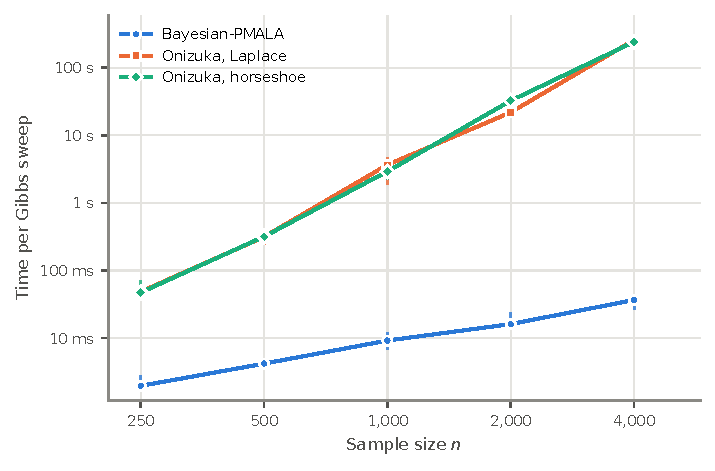
\includegraphics[width=0.7\textwidth]{figures/scal_time.pdf}
\caption{Median time per Gibbs sweep against $n$ (log--log), with bars spanning the range across replicates.}
\label{fig:cost_scaling}
\end{figure}

\paragraph{Results.} The time per sweep of Bayesian-PMALA grows linearly with $n$, at an essentially constant cost per observation, whereas an Onizuka sweep grows roughly cubically, so the gap widens with every doubling of $n$, from about one order of magnitude at the smallest $n$ to nearly four at the largest (Table~\ref{tab:cost_scaling}, Figure~\ref{fig:cost_scaling}). The two Onizuka priors cost the same. Almost all of a Bayesian-PMALA sweep is the P-MALA move, and almost all of an Onizuka sweep is the dense inverse and eigendecomposition of the trend draw (Figure~\ref{fig:cost_breakdown}).

The gap belongs to the supplied implementation rather than to the horseshoe hierarchy, whose precision matrix is banded and admits a banded Cholesky draw. The comparison concerns time per sweep, not the efficiency of the chains per sweep.

\begin{figure}[!htbp]
\centering
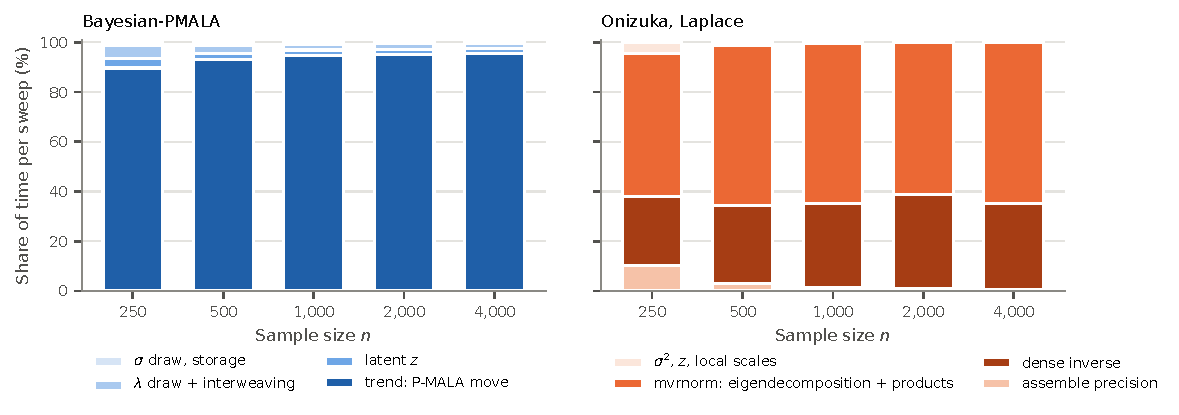
\includegraphics[width=\textwidth]{figures/scal_breakdown.pdf}
\caption{Share of the time per sweep spent in each update (median over replicates). Left: Bayesian-PMALA. Right: the Onizuka Laplace sampler; the horseshoe sampler's shares agree to within three percentage points.}
\label{fig:cost_breakdown}
\end{figure}

% !TeX root = ../main.tex
\subsection{Baseline recovery and peak detection in simulated air-quality data}
\label{sec:air_simulation}

We follow the peak-detection design of \citet[Section~4.2]{brantley2020baseline}, in which a slowly drifting baseline is contaminated by short-lived peaks. The goal is to estimate a low-quantile baseline and to detect the peaks in the detrended series. We compare Bayesian-PMALA with ADMM \citep{brantley2020baseline} and with the Laplace and horseshoe samplers of \citet{onizuka2024fast}, labeled Onizuka (Laplace) and Onizuka (Horseshoe) in Table~\ref{tab:air_n500}.

Each of $100$ replications has $n=500$ equally spaced observations. The baseline $b_i$ is a natural cubic spline with a random number of basis functions and independent $\operatorname{Exp}(1)$ coefficients. A $\operatorname{Binomial}(500,0.005)$ number of Gaussian-shaped peaks is placed at uniformly random locations, with widths drawn from $\operatorname{Unif}(2,12)$ and areas from $\mathcal{N}(20,4^2)$, and $s_i$ is their sum. The observations are $y_i=b_i+s_i+e_i$ with $e_i\stackrel{\mathrm{iid}}{\sim}\mathcal{N}(0,0.25^2)$. At each level $\tau\in\{0.01,0.05,0.10\}$, the estimand is the $\tau$-quantile of the peak-free series, $q_{\tau,i}=b_i+0.25\,\Phi^{-1}(\tau)$. Each method fits every level separately to the same $\by$; $b$ and $s$ are used only for evaluation.

This problem differs in structure from the simulations of Section~\ref{sec:simulations}: the data are a slowly varying baseline plus sparse, one-sided peaks, the working likelihood treats $s_i+e_i$ as the error, and the separation of baseline from peaks is not determined by the data alone, because a short peak can equally be read as a rough stretch of trend. With $a_0=1$, as in Section~\ref{sec:simulations}, the penalty settles where the roughness of the fitted trend puts it (Section~\ref{sec:theory-remarks}), and the fitted baseline bends into the peaks. In this section and in Section~\ref{sec:app:spod} we therefore use $\lambda\sim\mathrm{Gamma}(n,b_0)$: in the full conditional \eqref{eq:lambdaupdate}, $\mathrm{Gamma}(a_0+m,\ b_0+\norm{D\theta}_1)$, the shape $a_0=n$ adds $n$ to $m=n-k-1$ and so roughly doubles $\lambda$ at a given roughness of the trend. This heavier smoothing encodes the assumption that the baseline varies much more slowly than the peaks. In this simulation the fitted roughness $\norm{D\theta}_1$ is of the same order as $b_0$, so the prior and the data contribute about equally to both the shape and the rate of \eqref{eq:lambdaupdate}, and $b_0$ matters; it is chosen by the rule below. On the sensor data of Section~\ref{sec:app:spod} the roughness is much larger than $b_0$, and the posterior median of $\lambda$ changes by at most $12\%$ over the rates tried.

The rate $b_0=10^{-2}$ was chosen on this simulation by a rule fixed before the fits were run, over $b_0\in\{10^{-2},10^{-3},\dots,10^{-6}\}$ at each level, with the three chosen rates differing by at most a factor of ten. The value $b_0=10^{-2}$, the largest of the grid, was the only eligible rate at each level within one paired standard error of the smallest mean MSE, so no further ranking was needed. The sampler is that of the interior simulations (Appendix~\ref{app:pmala:settings}), run for $30{,}000$ sweeps with a burn-in of $10{,}000$, and the fitted curve is the posterior mean.

For a fitted curve $\widehat\theta_\tau$ we report the MSE against $q_\tau$ and the mean check loss (CL) on $\by$. Peaks are detected as the points with $y_i-\widehat\theta_{\tau,i}>h$, for $h\in\{0.5,0.75,1,1.2\}$, and compared with the true signal points $s_i>0.5$ by the class-averaged accuracy (CAA), the mean of sensitivity and specificity. Each metric is averaged over replications; CAA uses the $91$ replications that contain both signal and signal-free points.

\begin{table}[tb]
\centering
\small
\setlength{\tabcolsep}{4pt}
\caption{Simulated air-quality data, $n=500$ and $100$ replications. MSE is measured against the quantile of the peak-free series, CL is the mean check loss, and CAA is the class-averaged accuracy of peak detection at threshold $h$. Entries are means across replications. Bayesian-PMALA uses $\lambda\sim\mathrm{Gamma}(n,10^{-2})$. ADMM is refitted to the same data, the Onizuka (Laplace) entries are computed from archived fits to the same data, and the Onizuka (Horseshoe) entries are carried over unchanged from our original run of this design, whose per-replication results were not retained. $^{\dagger}$Average over $99$ replications ($90$ for CAA).}
\label{tab:air_n500}
\begin{tabular}{@{}rlrrrrrr@{}}
\toprule
 & & & & \multicolumn{4}{c}{CAA at threshold $h$} \\
\cmidrule(lr){5-8}
$\tau$ & Method & MSE & CL & $0.5$ & $0.75$ & $1$ & $1.2$ \\
\midrule
0.01 & Bayesian-PMALA & 0.0232 & 0.00663 & 0.713 & 0.840 & 0.832 & 0.764 \\
0.01 & ADMM & 0.0302 & 0.00642 & 0.687 & 0.818 & 0.838 & 0.780 \\
0.01 & Onizuka (Laplace) & 0.0980 & 0.00508 & 0.633 & 0.664 & 0.642 & 0.613 \\
0.01 & Onizuka (Horseshoe) & 0.0845 & 0.00541 & 0.619 & 0.670 & 0.656 & 0.627 \\
\addlinespace[3pt]
0.05 & Bayesian-PMALA & 0.0143 & 0.02870 & 0.793 & 0.859 & 0.799 & 0.720 \\
0.05 & ADMM$^{\dagger}$ & 0.0127 & 0.02925 & 0.792 & 0.876 & 0.825 & 0.743 \\
0.05 & Onizuka (Laplace) & 0.0848 & 0.02258 & 0.619 & 0.619 & 0.597 & 0.572 \\
0.05 & Onizuka (Horseshoe) & 0.1067 & 0.02354 & 0.579 & 0.580 & 0.556 & 0.534 \\
\addlinespace[3pt]
0.10 & Bayesian-PMALA & 0.0128 & 0.05034 & 0.839 & 0.847 & 0.762 & 0.684 \\
0.10 & ADMM & 0.0114 & 0.05130 & 0.843 & 0.870 & 0.789 & 0.706 \\
0.10 & Onizuka (Laplace) & 0.0651 & 0.04276 & 0.671 & 0.649 & 0.609 & 0.580 \\
0.10 & Onizuka (Horseshoe) & 0.1029 & 0.04166 & 0.572 & 0.551 & 0.533 & 0.517 \\
\bottomrule
\end{tabular}
\end{table}

Bayesian-PMALA and ADMM have comparable MSE at all three levels: $0.0232$, $0.0143$ and $0.0128$ at $\tau=0.01$, $0.05$ and $0.10$ for Bayesian-PMALA in Table~\ref{tab:air_n500}, against $0.0302$, $0.0127$ and $0.0114$ for ADMM. Over the replications common to both methods, the mean difference in MSE, Bayesian-PMALA minus ADMM, is $-0.0070$ (standard error $0.0041$) at $\tau=0.01$, $0.0015$ ($0.0014$) at $\tau=0.05$ and $0.0014$ ($0.0012$) at $\tau=0.10$, each within two standard errors of zero. The other metrics are mixed (Appendix~\ref{app:sim:air}). At $\tau=0.05$ and $0.10$, Bayesian-PMALA has a slightly lower check loss and a lower CAA at the thresholds $h\ge0.75$; at $\tau=0.01$, it has a higher check loss and a higher CAA at $h=0.5$ and $0.75$. The fits of the two samplers of \citet{onizuka2024fast} have the smallest check losses but the largest MSE, between $0.065$ and $0.107$, against at most $0.0302$ for Bayesian-PMALA and ADMM, and their CAA is lower than that of Bayesian-PMALA at every level and threshold. Between their two priors, the Laplace prior has the smaller MSE at $\tau=0.05$ and $0.10$ and the horseshoe at $\tau=0.01$. Small check losses with a large MSE are consistent with fits that follow the peaks rather than the baseline beneath them.

% !TeX root = ../main.tex
\subsection{Data applications}
\label{sec:applications}

We apply the individual sampler of Section~\ref{subsec:individual} to two real data sets, each with a frequentist benchmark. The first is one day of readings from a low-cost air-quality sensor, aggregated to $n = 8{,}640$ observations, where the target is a low quantile of the series that serves as its baseline. The second is the height of 4{,}817 boys and 5{,}190 girls aged 0 to 22 years from the Fifth Dutch Growth Study, where the target is a family of five quantile curves in age.

\subsubsection{Air-quality sensor data}
\label{sec:app:spod}

The first application is the fenceline monitoring problem for which \citet{brantley2020baseline} developed quantile trend filtering. The U.S.\ Environmental Protection Agency places low-cost SPod sensors on the perimeter of industrial facilities to detect fugitive emissions of volatile organic compounds. Each sensor records, once per second, the signal of a photoionization detector (PID) in uncalibrated counts. Emission plumes produce one-sided spikes lasting seconds to a few minutes, on a baseline that drifts over hours with temperature, humidity, and lamp condition. The baseline is therefore a low conditional quantile of the series, and it must be removed before events can be flagged or compared across sensors.

We analyze one day of data, June 15, 2018, from sensor \texttt{d} of the two collocated SPods in the EPA Rubbertown data set accompanying \citet{brantley2020baseline}. The day has $86{,}179$ usable 1-Hz readings; the other seconds are absent or, for $30$ consecutive seconds, recorded as not available. The readings are aggregated into 10-second means of the available readings, so that $n = 8{,}640$ ($19$ of the $8{,}640$ blocks, which contain no reading, are linearly interpolated). The aggregation attenuates the strong serial correlation of the 1-Hz noise, which the ALD working likelihood does not model.

We estimate the baseline at the three levels $\tau \in \{0.01, 0.05, 0.10\}$ with $k = 2$. Each level is fitted separately by the individual sampler on the standardized series, with the sampler and settings of Section~\ref{sec:air_simulation}. The series has the structure of that simulation, short one-sided plumes on a slowly varying baseline, and by the argument given there we use the same prior, $\lambda \sim \mathrm{Gamma}(n, 10^{-2})$ with $n = 8{,}640$. At each level we run two chains of $30{,}000$ sweeps with a burn-in of $10{,}000$, pool every $30$th retained draw of both, and report the pointwise posterior median, transformed back to counts. Under this prior the trend mixes slowly (Appendix~\ref{app:pmala:interior}), so the curves are reported as point estimates, without intervals.

As the frequentist benchmark we use the ADMM solver of the \texttt{detrendr} package of \citet{brantley2020baseline}. Its penalty is selected by extended BIC over the grid $\lambda \in \exp\{-2, \dots, 12\}$. The criterion selects $\lambda = 54.6$ at $\tau = 0.01$ and $\lambda = 1096.6$ at $\tau \in \{0.05, 0.10\}$. Following \citet{brantley2020baseline}, we detect events by a threshold rule on the detrended series $\by - \widehat{\theta}$: a point is classified as signal when it exceeds the empirical 90th, 95th, or 99th percentile of the detrended data. The rule requires no absolute calibration of the counts.

\begin{figure}[tbp]
\centering
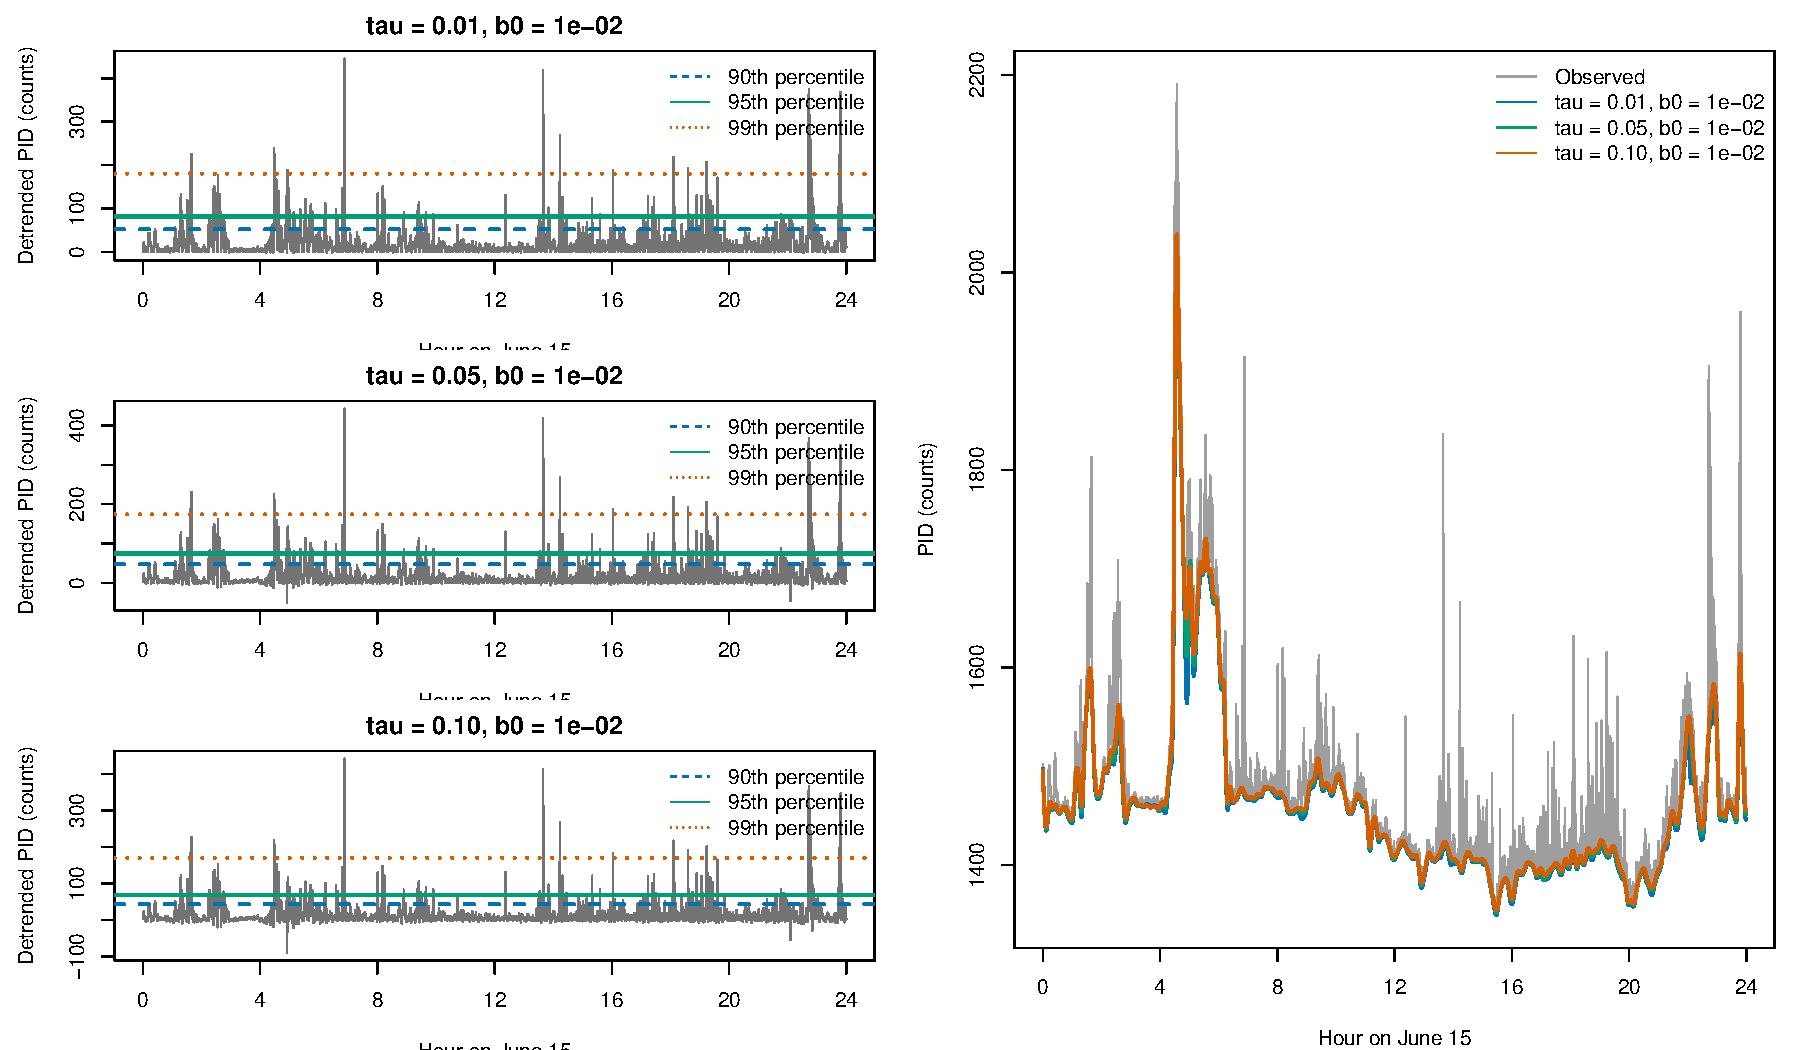
\includegraphics[width=\textwidth]{figures/spod_pmala_e18}
\caption{Air-quality data: Bayesian-PMALA fits with $k = 2$ and $\lambda \sim \mathrm{Gamma}(n, 10^{-2})$ on the 10-second means ($n = 8{,}640$) of SPod \texttt{d}, June 15, 2018. Left: detrended series $\by - \widehat{\theta}$, one panel per quantile level, with the 90th (dashed), 95th (solid), and 99th (dotted) empirical percentiles of the detrended data, the thresholds used to classify emission events. Right: baseline trends at $\tau \in \{0.01, 0.05, 0.10\}$, with the observed PID series in gray. Curves are pointwise posterior medians of two pooled chains.}
\label{fig:spod_pmala}
\end{figure}

The right panel of Figure~\ref{fig:spod_pmala} shows the three fitted baselines for Bayesian-PMALA; the ADMM fits and the detrended series they produce are in Appendix~\ref{app:spod_admm}. Both methods place most of the large excursion between 04:30 and 06:00 in the baseline, follow the slow decline through the afternoon, and leave the short plume spikes above the fit. The fraction of observations below the fitted curve is $0.009$, $0.059$, and $0.116$ at $\tau = 0.01, 0.05, 0.10$ for Bayesian-PMALA, against $0.000$, $0.043$, and $0.092$ for ADMM.

The three levels are fitted separately, so the curves are not constrained to be ordered, and they lie close together: the median distance between adjacent curves is about $1.5$ counts. At $1{,}097$ of the $8{,}640$ time points at least one adjacent pair is in the wrong order (the $0.01$ curve is above the $0.05$ curve at $812$ points, and the $0.05$ curve above the $0.10$ curve at $427$), by at most $6.3$ counts. The ADMM curves also cross: extended BIC selects a penalty twenty times smaller at $\tau = 0.01$ than at the other two levels, and the resulting curve bends upward into the plume near 05:00 and crosses the other two. The joint sampler of Section~\ref{subsec:joint}, which excludes crossings, was not run on these data.

The left panels of Figure~\ref{fig:spod_pmala} show the detrended series with the three detection thresholds, and Figure~\ref{fig:spod_detrended_admm} shows the ADMM counterpart. With the $\tau = 0.05$ baseline removed, the 95\% threshold is $74$ counts for Bayesian-PMALA and $92$ for ADMM, whereas the largest plume exceeds $400$ counts. The events of interest are therefore separated from the noise under either baseline.

Each chain of $30{,}000$ sweeps at $n = 8{,}640$ took between $37$ and $49$ minutes on one core of a Linux compute cluster. The ADMM fit with its grid search took roughly four minutes; it was not timed on the same machine, so the two times are not directly comparable.

\subsubsection{Growth centiles for Dutch children}
\label{sec:app:growth}

The second application is the growth chart: a child's height is read against the population centiles at the same age, so the chart is a family of quantile curves indexed by age. We use the Fifth Dutch Growth Study \citep{schonbeck2013tallest}, a nationwide cross-sectional sample collected in 2009 and distributed with the \texttt{mice} package \citep{vanbuuren2011mice}. After removing records without a height measurement, the data contain 4{,}817 boys and 5{,}190 girls aged 0 to 22 years, each measured once. Boys and girls are analyzed separately.

In contrast with the simulation designs, many children share a covariate value. We round age to the nearest tenth of a year, which gives a grid of $G = 220$ equally spaced ages for boys and $G = 221$ for girls, and index the trend $\theta \in \R^{G}$ by grid point. The ALD likelihood sums the check loss over all children at a grid point, so that each $\theta_g$ is informed by every height recorded at grid point $g$. In the augmented sampler each child keeps its own latent variable $z_i$, and the scale update \eqref{eq:sigmaupdate} runs over all children. In the trend target \eqref{eq:Utheta}, the Gaussian terms of the children at grid point $g$ combine into a single term in $\theta_g$, whose weight is the sum of their $w_i$ and whose center is the $w$-weighted mean of their $r_i$. Because the grid is equally spaced, the difference operator is the usual one, and the samplers apply without other changes.

We use $k = 2$ and $\lambda \sim \mathrm{Gamma}(1, \sqrt{G})$. Each level $\tau \in \{0.1, 0.3, 0.5, 0.7, 0.9\}$ is fitted by an independent run of 6{,}000 sweeps with 1{,}000 burn-in, and we report the posterior mean. This rate differs from those of the simulations, which have one observation per design point, because with some twenty children per grid point the likelihood is much more concentrated.

As a benchmark we fit the LMS method \citep{cole1992smoothing}, the standard tool for growth references. At each age, height is assumed to follow a Box--Cox Cole--Green distribution whose median, coefficient of variation, and Box--Cox power are smooth functions of age. All centiles are read off this one fitted distribution, so they cannot cross; the method assumes a parametric shape at every age. We use the \texttt{lms} function of the \texttt{gamlss} package \citep{rigby2005generalized}.

Figure~\ref{fig:growth_boys} shows the five fitted quantile curves for boys. The curves follow the fast growth in infancy, the near-linear childhood phase, the pubertal spurt, and the adult plateau, and they fan out with age as the height distribution widens. In-sample calibration is close to nominal: the fraction of boys below the fitted curve is $0.098$, $0.300$, $0.498$, $0.699$, and $0.903$ at $\tau = 0.1, 0.3, 0.5, 0.7, 0.9$.

The five fits are independent, so non-crossing is not enforced. The posterior-mean curves for girls do not cross. Those for boys cross in one of $880$ adjacent comparisons: at age $0.1$ years the $0.5$ curve lies $0.6$~cm above the $0.7$ curve.

The girls' fit and the LMS centiles for both sexes are in Appendix~\ref{app:growth} (Figures~\ref{fig:growth_girls}--\ref{fig:growth_lms_girls}). The two methods agree between about one and eighteen years of age and differ at the ends of the age range, where few children are observed. The LMS centiles follow the local data more closely. The trend filtering curves extrapolate the piecewise-quadratic trend: they lie slightly above the newborn measurements and bend at the oldest ages.

\begin{figure}[htbp]
\centering
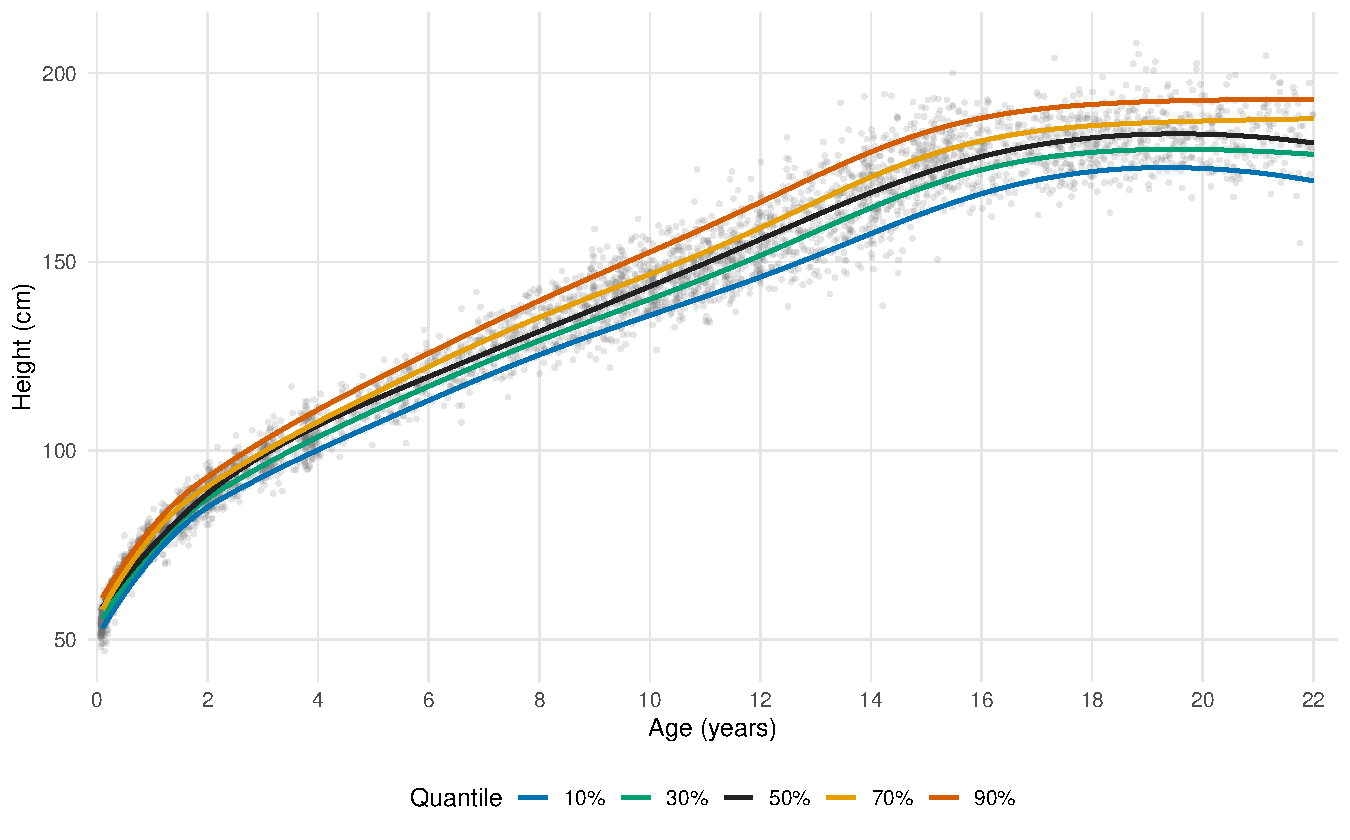
\includegraphics[width=0.75\textwidth]{figures/growth_pmala_boys}
\caption{Bayesian-PMALA fits for the height of 4{,}817 Dutch boys from the Fifth Dutch Growth Study \citep{schonbeck2013tallest} at $\tau \in \{0.1, 0.3, 0.5, 0.7, 0.9\}$, $k = 2$. Curves are posterior means on the 0.1-year age grid; gray circles are the individual measurements. Each level is fitted independently.}
\label{fig:growth_boys}
\end{figure}


% !TeX root = ../main.tex

\section{Conclusions}
\label{sec:discussion}

This paper proposes a Bayesian counterpart of the ADMM quantile trend filtering estimator: an asymmetric Laplace working likelihood and a Laplace prior with a global rate on the differences of the trend, with the penalty and the likelihood scale learned from the data. The posterior is sampled by a Gibbs sampler whose trend update is a P-MALA step on the whole conditional of the trend; its proximal map is a weighted trend filtering problem, every linear system is banded, and the cost per sweep grows linearly with $n$. For several quantile levels, the joint sampler restricts each trend to the box defined by its neighbors, and every draw is ordered. Theorem~\ref{thm:main} shows that, for a fixed scale and a fixed penalty of order $n^{(2k+1)/2}$, the posterior contracts around the true quantiles at the rate $n^{-(2k+1)/(2k+2)}$, and that this rate is exact. The result holds under two conditions on the distribution functions of the data near the quantile and does not assume the working likelihood.

The numerical results support the method. On the two benchmark signals, Bayesian-PMALA is competitive with the horseshoe sampler of \citet{onizuka2024fast} and with the ADMM estimator of \citet{brantley2020baseline}, and at extreme upper quantiles the fits of the joint sampler never cross. In the peak-detection design it performs close to ADMM, and its time per sweep grows linearly with $n$. In the two data applications, the same sampler estimates the baseline of an air-quality series with $n = 8{,}640$ observations and the growth centiles of Dutch children. A natural next step is a contraction result for the joint posterior of several quantile levels under the ordering constraint, which would extend Theorem~\ref{thm:main} to the non-crossing sampler.

% ----------------------------------------------------------------------------
% PARKED (W-04, 2026-11-24): the Discussion before the rewrite. The Conclusions above replace it.
% Possible homes: computational comparison -> Section 4 (computational cost); global penalty -> Section 4
% (peak detection); unknown sigma -> Section 3.3; joint target -> Section 2 (joint sampler).
% No home yet: the coverage remark and the list of extensions.
% Bayesian-PMALA brings exact posterior sampling to quantile trend filtering while keeping the proximal structure of the optimization problem. Under the normal--exponential representation, the proximal map of the whole conditional posterior of the trend is a weighted trend filtering problem, so no part of the check loss is smoothed and the Metropolis--Hastings correction is exact. In the simulation study each competitor is most accurate on the benchmark that suits it, and Bayesian-PMALA is competitive with both on both signals. It matches the locally adaptive horseshoe sampler with a single global penalty per quantile, and it matches ADMM while learning the penalty and the likelihood scale from the posterior instead of selecting a penalty by an information criterion.
%
% The computational structure is the second difference from the Gibbs sampler of \citet{onizuka2024fast}. Its supplied implementation forms a dense inverse and uses dense Gaussian simulation at each iteration, also with its sparse option. Every linear system in Bayesian-PMALA is banded, with bandwidth $k+1$ for every $n$. The metric $M$ and the ADMM system matrix change with $(z, \lambda, \sigma)$ and are therefore factorized at each sweep, but one factorization of each serves the forward and reverse proximal maps and the proposal noise, and for a fixed ADMM iteration budget the work per sweep grows linearly with $n$. The measured running times differ accordingly (Section~\ref{sec:scalability}): a sweep of the supplied implementation takes about $75$ times as long as a Bayesian-PMALA sweep at $n = 500$ and about $7\,000$ times as long at $n = 4000$. Running time per effective posterior draw also depends on mixing, which we do not compare here.
%
% The experiment of Section~\ref{sec:air_simulation} shows what the global penalty buys. There the target is a peak-free baseline beneath transient peaks, so local adaptivity is a liability: the horseshoe's local scales let the fit follow the peaks, whereas a single penalty cannot bend locally. Bayesian-PMALA is far more accurate than the horseshoe sampler on that design and close to ADMM.
%
% Treating the ALD scale $\sigma$ as unknown is a substantive modeling choice. At fixed $(\lambda, \sigma)$ the conditional mode is the quantile trend filter with penalty $\lambda\sigma$ \eqref{eq:map_qtf}, so the posterior learns the effective penalty through two parameters, the scale adapting to the noise level and $\lambda$ to the roughness of the trend, rather than asking one tuning parameter to absorb both roles. Learning $\sigma$ does not by itself guarantee frequentist coverage when the asymmetric Laplace likelihood is misspecified, a point also recognized by the calibration approach of \citet{onizuka2024fast}.
%
% A single global penalty is a deliberate simplification relative to coefficient-specific shrinkage, and the experiments do not establish a universally preferred prior or difference order. The pointwise intervals are below nominal coverage at the outer quantile levels (Section~\ref{sec:sim:ind:smooth}), and their calibration there requires further study.
%
% The joint sampler of Section~\ref{subsec:joint} enforces non-crossing on every posterior draw at the observed indices, and it does so without leaving the P-MALA framework: the order constraint adds the indicator of a box to the negative log-conditional of each trend, which keeps it convex, so only the proximal map changes and the Metropolis--Hastings correction keeps its single-level form. The joint target is a constrained product of working posteriors for the same data, not a joint likelihood for several quantiles, and how the constraint shifts each level's posterior relative to its single-level fit, in location and in interval width, remains to be studied.
%
% Several extensions follow from the present work. Locally adaptive priors can be combined with the same proximal update, since the conditional of the trend remains a weighted quadratic plus a weighted $\ell_1$ penalty. Extension to spatially indexed signals requires generalizing the difference operator to graphs, for which the systems are no longer banded and sparse or multigrid solvers may serve a similar role. Finally, the convergence properties of the full Gibbs sampler with continuous step-size adaptation remain to be established.
% ----------------------------------------------------------------------------

\clearpage
\appendix
\section{Proofs of the theoretical results}\label{app:proofs}
[TODO W-04 phase 2.]

\section{Analysis of the assumptions}\label{app:assumptions}
[TODO W-04 phase 2.]

% !TeX root = ../main.tex
\section{Computational details of Bayesian-PMALA}
\label{app:pmala}

\subsection{Full conditional distributions}
\label{app:pmala:conditionals}

Write $e_i = y_i - \theta_i$. For $z_i$, expanding the square in \eqref{eq:posterior} and dropping the cross term $-\psi_\tau e_i/(\omega_\tau^2\sigma)$, which does not depend on $z_i$, gives
\[
p(z_i \mid \theta, \sigma, \by) \propto z_i^{-1/2} \exp\!\left\{-\frac{1}{2}\left(\frac{\chi_i}{z_i} + \tilde\psi\, z_i\right)\right\},
\qquad \chi_i = \frac{e_i^2}{\omega_\tau^2 \sigma}, \quad \tilde\psi = \frac{1}{\sigma}\left(\frac{\psi_\tau^2}{\omega_\tau^2} + 2\right),
\]
a generalized inverse Gaussian distribution $\mathrm{GIG}(1/2, \chi_i, \tilde\psi)$, with $\tilde\psi = 1/\{2\tau(1-\tau)\sigma\}$. For $e_i \ne 0$ its reciprocal is inverse Gaussian with mean $(\tilde\psi/\chi_i)^{1/2} = 1/\{\tau(1-\tau)|e_i|\}$ and shape $\tilde\psi$, which is \eqref{eq:zupdate}; for $e_i = 0$, $z_i$ is Gamma distributed with shape $1/2$ and rate $\tilde\psi/2$, a case that safeguard~(i) of Appendix~\ref{app:pmala:safeguards} excludes. The terms involving $\lambda$ are $\lambda^{a_0+m-1}\exp\{-\lambda(b_0 + \norm{D\theta}_1)\}$, which gives \eqref{eq:lambdaupdate}. The factors $\sigma^{-n/2}$ and $\sigma^{-n}$ from the Gaussian and exponential densities and the inverse-Gamma prior give \eqref{eq:sigmaupdate}.

\subsection{The proximal map of the individual sampler}
\label{app:pmala:admm}

Write the metric \eqref{eq:metric} as $M = \mathrm{diag}(d) + cD^\top D$, with $d = w$ and $c = \min(\kappa\lambda^2/2, 10^8)$, the cap being safeguard~(ii) of Appendix~\ref{app:pmala:safeguards}. Problem \eqref{eq:prox} is the minimization over $(\theta, v)$ of $\frac12\sum_i w_i(\theta_i - r_i)^2 + \lambda\norm{v}_1 + \norm{\theta - x}_M^2/(2\gamma)$ subject to $v = D\theta$. We apply scaled ADMM with penalty $\varrho > 0$ and scaled dual variable $\nu \in \R^m$. Starting from $v^0 = Dx$ and $\nu^0 = 0$, iteration $t$ is
\begin{align*}
\theta^{t+1} &= x + A^{-1}\left\{ W(r - x) + \varrho D^\top (v^t - \nu^t - Dx) \right\}, \qquad A = W + \gamma^{-1} M + \varrho D^\top D, \\
v^{t+1} &= \mathcal{S}_{\lambda/\varrho}\!\left(D\theta^{t+1} + \nu^t\right), \qquad
\nu^{t+1} = \nu^t + D\theta^{t+1} - v^{t+1},
\end{align*}
where $\mathcal{S}_a(b) = \mathrm{sign}(b)\max(|b| - a, 0)$ acts elementwise. The $\theta$-update is the usual one, $A\theta^{t+1} = Wr + \gamma^{-1}Mx + \varrho D^\top(v^t - \nu^t)$, solved for the increment $\theta^{t+1} - x$: its right-hand side scales with the move $T(x) - x$ rather than with $\gamma^{-1}Mx$, so its rounding error does not grow like $1/\gamma$ in the acceptance ratio \eqref{eq:pmala_accept}. We use $\varrho = 0.1\,(\bar w + c)/\gamma$ with $\bar w = n^{-1}\sum_i w_i$, about one tenth of the curvature of the metric term, and return $\theta^{150}$, with no data-dependent stopping rule.

The matrices $A$ and $M$ are symmetric positive definite and banded with half-bandwidth $k+1$. Within one move $A$ does not depend on $x$, so one banded Cholesky factor serves the forward map $T(\theta)$ and the reverse map $T(\theta^\star)$. The metric is factorized once per move as $M = LL^\top$ for the noise in \eqref{eq:pmala_proposal}, and the norms in \eqref{eq:pmala_accept} are evaluated as $\norm{b}_M^2 = \sum_i d_i b_i^2 + c\norm{Db}_2^2$. A factorization costs $O(n(k+1)^2)$ operations and an ADMM iteration $O(n(k+1))$.

The correction \eqref{eq:pmala_accept} requires only that $T$ be a deterministic function of its input, given $(z, \lambda, \sigma, \delta)$ (Section~\ref{subsec:pmala}). The cold start from $(Dx, 0)$ and the fixed iteration rule, used for the forward and the reverse map, guarantee this, whereas a warm start from the previous sweep would not. For the same reason the noise is added after the proximal map: added before it, it would give the image of a Gaussian under a nonlinear map, whose density is not available.

\subsection{The proximal map of the joint sampler}
\label{app:pmala:boxsolver}

Fix a level and suppress its index. The box $B = [\ell, u]$ of \eqref{eq:joint_box} may have infinite components (at $j = 1$ and $j = J$), and $\ell_i = u_i$ is allowed where two neighboring curves touch; such coordinates are fixed at their bound and eliminated. We write $T_B$ for the map \eqref{eq:joint_prox}, the proximal map of $U + \iota_B$ in the $M$-norm. The smooth part of its objective has Hessian $A_0 = W + M/\gamma$, so on the free coordinates the problem is strongly convex with modulus at least $\varpi = \min_{i:\,\ell_i < u_i}(w_i + d_i/\gamma)$. We write $\widehat T_B$ for the map actually computed, the $T_j$ of \eqref{eq:joint_proposal}--\eqref{eq:joint_accept}.

\paragraph{Stage 1: the unbounded map.} The solver first computes $\tilde\theta = T(x)$ by the ADMM of Appendix~\ref{app:pmala:admm}, with the same penalty, cold start and budget, and returns this iterate, the output of a fixed number of ADMM iterations, whenever it is feasible, $\ell \le \tilde\theta \le u$. The rule mirrors the fact that an exact unbounded minimizer lying in $B$ is also the constrained minimizer. Hence $\widehat T_B$ coincides bitwise with the individual map for a free box ($J = 1$) and whenever the computed $\tilde\theta$ lies in $B$.

\paragraph{Stage 2: an interior-point method.} Otherwise $T_B(x)$ is computed from the epigraph quadratic program
\begin{equation}
\begin{aligned}
\min_{\theta \in \R^n,\ \upsilon \in \R^m}\ & \tfrac12\theta^\top A_0\theta + \beta^\top\theta + \lambda\mathbf 1^\top\upsilon \\
\text{subject to}\ & D\theta - \upsilon \le 0, \quad -D\theta - \upsilon \le 0, \quad \theta_i \le u_i\ (u_i < \infty), \quad \ell_i - \theta_i \le 0\ (\ell_i > -\infty),
\end{aligned}
\label{eq:box_qp}
\end{equation}
with $\beta = -(Wr + Mx/\gamma)$, which is equivalent to \eqref{eq:joint_prox} because $\upsilon = |D\theta|$ at the optimum. We solve \eqref{eq:box_qp} by Mehrotra's predictor--corrector primal--dual method \citep{mehrotra1992implementation}, with slacks $s_1, \ldots, s_4$ and multipliers $\mu_1, \ldots, \mu_4$ for the four constraint blocks. Eliminating the slack and multiplier steps and, through the $\upsilon$-row of the Newton equations, the step in $\upsilon$, leaves one linear system in $\Delta\theta$ with matrix $A_0 + D^\top \Lambda_\upsilon D + \Lambda_3 + \Lambda_4$, where $\Lambda_l = \mathrm{diag}(\mu_l/s_l)$, $l = 1, \ldots, 4$, and $\Lambda_\upsilon = 4\Lambda_1\Lambda_2(\Lambda_1 + \Lambda_2)^{-1}$, which is symmetric positive definite and banded with half-bandwidth $k+1$. In each iteration the predictor and the corrector each factorize it by banded Cholesky, in $O(n(k+1)^2)$ operations, and solve with it, with centering parameter $\min\{1, (\bar\mu_{\mathrm{aff}}/\bar\mu)^3\}$, where $\bar\mu = s^\top\mu/N$ over the $N$ inequality constraints and $\bar\mu_{\mathrm{aff}}$ is its value after the predictor step. Separate primal and dual step lengths in $(0, 1]$ keep $0.99$ of the distance to the boundary.

\paragraph{Initialization and stopping.} The method starts from $\theta^0 = \min\{\max(\tilde\theta, \ell), u\}$, $\upsilon^0 = |D\theta^0| + s_{\min}$, slacks at least $s_{\min} = 0.01\,s_\theta$, $s_\theta = \max(1, \norm{\theta^0}_\infty)$, $\mu_1 = \mu_2 = \lambda/2 + 10^{-8}$ and box multipliers $1$. With $\varepsilon = 10^{-8}$, the thresholds are $\varepsilon(1 + s_\theta)$ for the primal residual, $\varepsilon\varpi$ for the dual residual and $\varepsilon^2\varpi/2$ for $s^\top\mu$. With $\phi$ the largest ratio of a residual to its threshold, the iterate with the smallest $\phi$ is retained, clipped to $B$ and returned when $\phi \le 1$, on stall ($10$ iterations after the $15$th without a $10\%$ reduction of the best $\phi$), on a non-finite value, or after $100$ iterations. In the sampler $\varepsilon\varpi$ is at the rounding level of $A_0\theta + \beta$, so the loop usually ends on stall. These are stopping criteria, not error bounds; the accuracy of the output is checked in Appendix~\ref{app:pmala:tests}.

\paragraph{Determinism.} Every rule above depends only on $(x, w, r, \lambda, d, c, \gamma, \ell, u)$ and on the iterates, so $\widehat T_B$ is a deterministic function of $x$ and the correction \eqref{eq:joint_accept} is exact for the computed map. The forward and reverse maps of a move use the same box, metric, step size and rule.

\subsection{Interweaving step for the penalty}
\label{app:pmala:asis}

The conjugate draw \eqref{eq:lambdaupdate} is followed by a draw in the ancillary parameterization \citep{yu2011center}. Let $Q \in \R^{n\times(k+1)}$ be an orthonormal basis of the null space of $D$, and write $\theta = p + v$ with $p = QQ^\top\theta$. Under \eqref{eq:prior_theta} the standardized differences $\lambda D\theta = \lambda Dv$ have independent standard Laplace entries and do not depend on $\lambda$. Holding them and $(p, z, \sigma)$ fixed, a new value $\lambda'$ implies the trend $\theta(\lambda') = p + (\lambda/\lambda')v$. The factor $\lambda'^m$ in \eqref{eq:prior_theta} cancels the Jacobian of $v \mapsto \lambda' Dv$, so $\eta = \log\lambda'$ has log density
\begin{equation}
\log f(\eta) = a_0\eta - b_0 e^\eta - \frac12\sum_{i=1}^n w_i\left\{\theta_i(e^\eta) - r_i\right\}^2 ,
\label{eq:asis_density}
\end{equation}
where $a_0\eta$ includes the factor $e^\eta$ from the change of variables. We draw $\eta$ by slice sampling \citep{neal2003slice} with initial width $1$, at most $30$ stepping-out steps divided at random between the two ends, and shrinkage, leaving the state unchanged if the interval shrinks below width $10^{-10}$, and set $\theta \leftarrow \theta(\lambda')$. The conjugate and the ancillary draws each leave \eqref{eq:posterior} invariant, and so does their composition.

\paragraph{Constrained version for the joint sampler.} At level $j$, with $p$ and $v$ as in \eqref{eq:joint_asis_curve} and the index dropped, the rescaled trend $p + \varphi v$, $\varphi = \lambda/\lambda' > 0$, lies in $B_j$ if and only if $\ell_i \le p_i + \varphi v_i \le u_i$ for every $i$. For $v_i \ne 0$ this is an interval in $\varphi$ with endpoints $(\ell_i - p_i)/v_i$ and $(u_i - p_i)/v_i$, and for $v_i = 0$ it requires $p_i \in [\ell_i, u_i]$. The intersection of these intervals with $(0, \infty)$ is $[\varphi_-, \varphi_+]$, with endpoints $0$ or $\infty$ allowed, and
\begin{equation}
\log\lambda - \log\varphi_+\ \le\ \eta\ \le\ \log\lambda - \log\varphi_- .
\label{eq:joint_asis_interval}
\end{equation}
The slice update targets \eqref{eq:asis_density} restricted to \eqref{eq:joint_asis_interval}, with the weights and pseudo-responses of the newly drawn $z_j$ and the current $\sigma_j$. The reconstructed trend is also checked against the box, so that rounding cannot produce a crossing, and is never clipped. If the interval is empty or degenerate, or the current density is not finite, the state is left unchanged.

\subsection{Initialization, adaptation and safeguards}
\label{app:pmala:init}
\label{app:pmala:adapt}
\label{app:pmala:safeguards}

\paragraph{Initialization and warm-up.} In the algorithm of Section~\ref{sec:methodology}, every chain of the individual sampler starts at $\theta^{(0)} = \by$, with $\sigma^{(0)} = 1$, $z_i^{(0)} = \sigma^{(0)}$, $\lambda^{(0)} = m$ and $\delta^{(0)} = 0.2$. These data-free values avoid the conditionals given $\theta = \by$, which place $\sigma$ and $z$ near zero, a configuration from which a Gibbs chain moves away only slowly. For $J > 1$ the joint sampler starts the trends at $\theta_j^{(0)} = \by + s_y\{\Phi^{-1}(\tau_j) - \mathrm{median}_{h}\,\Phi^{-1}(\tau_h)\}\mathbf 1$, with $s_y = \max\{\mathrm{sd}(\by), 0.1\}$ and $\Phi$ the standard normal distribution function, so that the levels start strictly ordered; the other parameters start as in the individual sampler.

From $\theta = \by$ an exact Metropolis--Hastings chain barely moves: proposals are close to the output of a proximal map, which is smooth in $D\theta$, so for the rough $\by$ the reverse term $\norm{\by - T(\theta^\star)}_M^2/(2\delta)$ in \eqref{eq:pmala_accept} can make the acceptance probability of a proposal negligible. The first $H = 200$ sweeps therefore replace the P-MALA move by the proximal-point step $\theta \leftarrow \arg\min_{\vartheta}\{U(\vartheta) + \norm{\vartheta - \theta}_W^2/(2\gamma_{\mathrm{w}})\}$, $\gamma_{\mathrm{w}} = 10^4$, approximated by $300$ iterations of the ADMM of Appendix~\ref{app:pmala:admm} with $M = W$, $\gamma = \gamma_{\mathrm{w}}$ and $\varrho = \mathrm{median}(w_i)$. In the joint sampler the step is restricted to the current box, that is \eqref{eq:joint_prox} with $M_j = W_j$ and $\gamma_{\mathrm{w}}$, and computed as in Appendix~\ref{app:pmala:boxsolver} with the same budget, which keeps the levels ordered. The blocks $z$, $\lambda$ and $\sigma$ are drawn as usual during the warm-up; the interweaving step and the step-size adaptation start after it. The warm-up is part of the burn-in.

\paragraph{Step-size adaptation.} After the warm-up the step size is updated at every sweep by $\log\delta_{t+1} = \log\delta_t + t^{-0.6}\{\min(1, \alpha_t) - 0.5\}$, with $\alpha_t$ from \eqref{eq:pmala_accept}, and $\delta$ is confined to $[10^{-8}, 10^{2}]$. The adaptation continues after burn-in, because $\lambda$ can still drift slowly in the retained sweeps and a frozen step size would let the acceptance rate drift with it; the vanishing gain satisfies the diminishing-adaptation condition of \citet{roberts2007coupling}. In the joint sampler each level has its own $\delta_j$, and a proposal outside $B_j$ counts as $\alpha_t = 0$.

\paragraph{Safeguards.} (i) Each draw $z_i$ is restricted to $[10^{-8}, 10^{4}]$, and $|y_i - \theta_i|$ is floored at $10^{-10}$ in \eqref{eq:zupdate}, so that $M$ and the solver systems can be factorized. (ii) The coefficient $\kappa\lambda^2/2$ in \eqref{eq:metric} is capped at $10^{8}$. (iii) If a banded Cholesky factorization fails because of rounding, a ridge $\epsilon\max_i A_{ii}$ is added to the diagonal, starting from $\epsilon = 10^{-12}$ and multiplying $\epsilon$ by $100$ up to five times; the ridge is part of the solver, so the proximal map remains deterministic. (iv) A non-finite $\log\alpha$ is treated as a rejection, and a non-finite state stops the run with an error. The joint sampler also verifies after every update of a level that the trend lies in its box, and a violation stops the run.

The Metropolis--Hastings argument of Section~\ref{subsec:pmala} covers (ii) and (iii), which change only the proposal, and the box check, which never triggers when the kernels are implemented correctly. It does not cover (i): clipping the latent draws and flooring the residual alter the conditional of $z$ slightly, and clipping is not sampling from a normalized truncated distribution, so the sampler targets \eqref{eq:posterior} or \eqref{eq:joint_target} up to the clipping of the latent draws; the trend update itself remains exact.

\subsection{Settings of each experiment}
\label{app:pmala:settings}

The algorithm of Section~\ref{sec:methodology} uses $\kappa = 3$, $a_\sigma = b_\sigma = 0.1$, $\delta^{(0)} = 0.2$, $\lambda^{(0)} = m$, $\sigma^{(0)} = 1$, $H = 200$, $\gamma_{\mathrm{w}} = 10^4$, $150$ ADMM iterations, and gain $t^{-0.6}$ toward acceptance $0.5$ with $\delta \in [10^{-8}, 10^2]$. Table~\ref{tab:pmala_settings} lists, for each result, the settings recorded for its runs.

\begin{table}[htbp]
\centering
\footnotesize
\caption{Sampler settings of each experiment. Target: acceptance target. ADMM: form of the $\theta$-update (Appendix~\ref{app:pmala:admm}). ---: not recorded. $^{a}$Levels $0.96$--$0.99$. $^{b}$Levels $0.90$ and $0.93$, from a second run with the same sampler and kernel code, whose run configuration was not recorded. $^{c}$Prior $\lambda\sim\mathrm{Gamma}(n, 10^{-2})$, that is, $a_0 = n$; the SPod fits use two chains per level.}
\label{tab:pmala_settings}
\setlength{\tabcolsep}{2.5pt}
\begin{tabular}{@{}llllllll@{}}
\toprule
Result & Section & Version & $b_0$ (VS / S) & Sweeps/burn-in & Interweaving & Target & ADMM \\
\midrule
Interior & \ref{sec:sim:individual} & App.~\ref{app:pmala:interior} & $10^{-3}$ / $5\times10^{-4}$ & $30000/10000$ & spline-held & $0.5$ & increment \\
Extreme, individual$^{a}$ & \ref{sec:sim:extreme} & Sec.~\ref{sec:methodology} & $10^{-2}$ / $10^{-3}$ & $10000/3000$ & off & $0.55$ & increment \\
Extreme, individual$^{b}$ & \ref{sec:sim:extreme} & Sec.~\ref{sec:methodology} & --- & --- & --- & --- & increment \\
Extreme, joint & \ref{sec:sim:extreme} & Sec.~\ref{sec:methodology} & $10^{-2}$ / $10^{-3}$ & $30000/10000$ & on & $0.5$ & increment \\
Air simulation & \ref{sec:air_simulation} & App.~\ref{app:pmala:interior} & $10^{-2}$\,$^{c}$ & $30000/10000$ & spline-held & $0.5$ & increment \\
SPod data & \ref{sec:app:spod} & App.~\ref{app:pmala:interior} & $10^{-2}$\,$^{c}$ & $30000/10000$ & spline-held & $0.5$ & increment \\
Growth data & \ref{sec:app:growth} & --- & $\sqrt{G}$ & $6000/1000$ & --- & --- & --- \\
Timings & \ref{sec:scalability} & --- & --- & --- & --- & --- & --- \\
\bottomrule
\end{tabular}
\end{table}

\subsection{Version of the sampler used for the interior simulations and the air-quality fits}
\label{app:pmala:interior}

The interior-quantile results of Section~\ref{sec:sim:individual} use a version of the individual sampler that differs from the algorithm above in the starting values, the treatment of $\lambda$ during the warm-up, the interweaving step and two safeguards. The air-quality fits of Sections~\ref{sec:air_simulation} and~\ref{sec:app:spod} use the same version, with the prior $\lambda\sim\mathrm{Gamma}(n, 10^{-2})$.

\paragraph{Start and warm-up.} With window length $\max(5,\,2\lfloor n/40\rfloor+1)$, which is $25$ at $n = 500$, let $\theta^{\mathrm{rm}}$ be the running median of $\by$, and let $\hat q_\tau$ be the empirical $\tau$-quantile of $\by - \theta^{\mathrm{rm}}$. The chain starts at $\theta^{(0)} = \theta^{\mathrm{rm}} + \hat q_\tau\mathbf 1$, with $\sigma^{(0)} = n^{-1}\sum_i\rho_\tau(y_i - \theta^{(0)}_i)$, the maximum-likelihood ALD scale given $\theta^{(0)}$, with $z^{(0)}$ drawn from \eqref{eq:zupdate} given $(\theta^{(0)}, \sigma^{(0)})$, and with $\lambda^{(0)} = m$. In each warm-up sweep the proximal-point step is computed by the ADMM of Appendix~\ref{app:pmala:admm} if its relative residual falls below $10^{-6}$, and otherwise by the interior-point method of Appendix~\ref{app:pmala:boxsolver} with $\varepsilon = 10^{-8}$ and at most $200$ iterations; in the interior simulations the interior-point method was used at every warm-up sweep. In three replayed interior-simulation runs, in the $300$ air-quality simulation fits of Table~\ref{tab:air_n500} and in the six chains fitted to the SPod data, it was used at each of the $200$ warm-up sweeps and stopped before reaching its tolerance at every one of them, so the warm-up, whose purpose is to move the chain away from its start, applies an approximate proximal-point step and is discarded with the burn-in. The draws of $z$ and $\sigma$ are unchanged, but $\lambda$ is held at $\lambda^{(0)}$; its conjugate draw and the interweaving step start at sweep $H + 1$.

\paragraph{Interweaving step.} Let $P_q$ be the orthogonal projection onto the span of $q$ cubic B-splines with equally spaced knots on the design points $i/n$, a space that contains the polynomials of degree at most $k$, and write $\theta = p + v$ with $p = P_q\theta$. A new value $\lambda'$ gives $\theta(\lambda') = p + (\lambda/\lambda')v$, and $\eta = \log\lambda'$ is drawn by the slice sampler of Appendix~\ref{app:pmala:asis} from
\[
(a_0 + q - k - 1)\,\eta - b_0 e^{\eta} - \norm{e^{\eta}Dp + \lambda Dv}_1 - \frac12\sum_{i=1}^n w_i\left\{\theta_i(e^{\eta}) - r_i\right\}^2 .
\]
Its exponent collects $a_0 - 1 + m$ from the prior, $1$ from the change of variables and $-(n - q)$ from the rescaling of $v$. For $q > k+1$, $Dp$ can be nonzero, so the step is not an ancillary draw but a generalized Gibbs move \citep{liu2000generalised}: the transformations $(\lambda, \theta) \mapsto (e^{t}\lambda,\, p + e^{-t}v)$, $t \in \R$, form a group, the density above is the conditional of $\eta = \log\lambda + t$ that their construction prescribes, and the step leaves \eqref{eq:posterior} invariant. For $q = k+1$ it is the step of Appendix~\ref{app:pmala:asis}. The dimension $q$ cycles through $10$, $20$ and $40$, one value per sweep, and the fixed cycle also leaves the posterior invariant.

\paragraph{Safeguards and diagnostics.} In safeguard~(i) the floor on $|y_i - \theta_i|$ is $10^{-100}$, and the inverse Gaussian draw in \eqref{eq:zupdate} is computed in a form that avoids cancellation and has the same distribution. During the burn-in only, a draw of $\sigma$ larger than $10\sigma^{(0)}$ is replaced by $\sigma^{(0)}$. Over the $3000$ interior runs this reset was never triggered, no run stopped, and the post-burn-in acceptance rate was between $0.486$ and $0.520$. The median wall time per run was $153$ seconds on one core of a Linux compute cluster, and the median effective sample size of $\log\lambda$, from every $30$th retained draw, was $102$ for the VS signal and $132$ for the S signal. For the air-quality fits under the prior $\mathrm{Gamma}(n, 10^{-2})$ the trend mixes slowly; we report the posterior mean in the simulation and the posterior median for the SPod data as point estimates, and for the SPod data we pool two chains.

\subsection{Exactness checks}
\label{app:pmala:tests}

\paragraph{Individual sampler.} Tests check the identity \eqref{eq:ald_mixture}; the GIG conditional of $z_i$; the proximal map against the \texttt{glmgen} solver \citep{tibshirani2014adaptive} at $M = \mathbf{I}_n$, and its minimizing property in the metric \eqref{eq:metric}; the trend move against the exact Gaussian conditional at $\lambda = 0$ and against grid integration at $n = 4$; the shared-factorization move against separate solves; and the interweaving chain against grid integration. At $n = 7$ the step of Appendix~\ref{app:pmala:interior} with $q \in \{4, 5, 6\}$ agreed with an importance-sampling reference, which detected a deliberately wrong coefficient of $\eta$.

\paragraph{Joint sampler.} At $\lambda = c = 0$, $\widehat T_B$ matches the closed-form separable solution to $8.5\times10^{-12}$. Its objective was never above that of the solver Clarabel \citep{goulart2024clarabel} on $108$ small problems, and above it by at most $1.9\times10^{-9}$ relative on $72$ problems that reproduce the conditions of the sampler; on the $66$ that reached stage~2, a tighter tolerance moved the output by at most $4\times10^{-9}$ proposal-noise standard deviations, and an independent ADMM came within $0.033$ such standard deviations. With $J = 1$ and a common seed the joint sampler reproduces the individual sampler exactly on the same machine. At $n = 4$, with a box that cuts into the bulk of the conditional, the constrained trend move, alone and with the draw of $\lambda$ and the constrained interweaving step, agrees with integration on an $80^4$ midpoint grid (batch-means $z$-scores at most $1.9$; $E(\lambda) = 1.089 \pm 0.004$ against the exact $1.090$). A three-level run ($n = 80$, $\tau \in \{0.5, 0.9, 0.95\}$) has no crossing in any retained draw.

% !TeX root = ../main.tex
\providecommand{\tbc}[1]{\textcolor{red}{[TBC: #1]}}
\section{Additional simulation results}
\label{app:simulation_results}

This appendix supplements Section~\ref{sec:simulations} ($n=500$, $k=2$): Appendix~\ref{app:sim:individual} reports interior-quantile MAD and MCIW for Section~\ref{sec:sim:individual}, and Appendix~\ref{app:sim:joint_extreme} reports extreme-quantile crossing counts for Section~\ref{sec:sim:extreme}. All entries are averages over valid replications.

\subsection{Interior quantiles}
\label{app:sim:individual}
\label{app:sim:individual:vs}
\label{app:sim:individual:smooth}

For the VS signal (Table~\ref{tab:vs_int_mad_mciw}), Bayesian-PMALA produces narrower $95\%$ intervals than both samplers of \citet{onizuka2024fast} in every configuration; the MAD ranking of the four methods differs from the MSE ranking of Table~\ref{tab:vs_int_mse} in four of the $15$ configurations. For the S signal (Table~\ref{tab:s_int_mad_mciw}), Bayesian-PMALA has smaller MAD and narrower intervals than both samplers of \citet{onizuka2024fast} in every configuration.

\begin{table}[htbp]
\centering
\scriptsize
\renewcommand{\arraystretch}{0.95}
\setlength{\tabcolsep}{2.4pt}
\caption{Interior-quantile MAD and MCIW for the VS signal (ADMM unavailable, --).}
\label{tab:vs_int_mad_mciw}
\begin{tabular}{@{}lrrrrrrrrrr@{}}
\toprule
 & \multicolumn{5}{c}{MAD} & \multicolumn{5}{c}{MCIW} \\
\cmidrule(lr){2-6}\cmidrule(l){7-11}
Method & $0.05$ & $0.25$ & $0.50$ & $0.75$ & $0.95$ & $0.05$ & $0.25$ & $0.50$ & $0.75$ & $0.95$ \\
\midrule
\multicolumn{11}{@{}l}{\textit{Beta}} \\
Onizuka (Laplace) & 0.012702 & 0.020517 & 0.030557 & 0.040591 & 0.066465 & 0.072159 & 0.100837 & 0.132473 & 0.158571 & 0.168685 \\
Onizuka (Horseshoe) & 0.011300 & 0.018849 & 0.028763 & 0.038443 & 0.062328 & 0.067523 & 0.100344 & 0.134284 & 0.161300 & 0.166118 \\
Bayesian-PMALA & 0.012705 & 0.020700 & 0.030584 & 0.040697 & 0.069261 & 0.063096 & 0.097263 & 0.128918 & 0.154285 & 0.159541 \\
ADMM & 0.027314 & 0.029267 & 0.044214 & 0.052848 & 0.076817 & -- & -- & -- & -- & -- \\
\addlinespace[3pt]
\multicolumn{11}{@{}l}{\textit{Mixed normal}} \\
Onizuka (Laplace) & 0.215556 & 0.139979 & 0.128822 & 0.138850 & 0.215747 & 0.557248 & 0.564334 & 0.569489 & 0.565218 & 0.559566 \\
Onizuka (Horseshoe) & 0.212371 & 0.140284 & 0.129614 & 0.141514 & 0.218726 & 0.578243 & 0.613924 & 0.620905 & 0.624492 & 0.599896 \\
Bayesian-PMALA & 0.216900 & 0.139086 & 0.126371 & 0.137381 & 0.209422 & 0.533499 & 0.515367 & 0.511419 & 0.516501 & 0.527685 \\
ADMM & 0.218535 & 0.183889 & 0.169139 & 0.157936 & 0.201602 & -- & -- & -- & -- & -- \\
\addlinespace[3pt]
\multicolumn{11}{@{}l}{\textit{Gaussian}} \\
Onizuka (Laplace) & 0.109980 & 0.070160 & 0.063856 & 0.067192 & 0.103017 & 0.289501 & 0.286599 & 0.285566 & 0.284948 & 0.280193 \\
Onizuka (Horseshoe) & 0.106356 & 0.068189 & 0.061950 & 0.065668 & 0.101007 & 0.296111 & 0.301798 & 0.301683 & 0.301976 & 0.290053 \\
Bayesian-PMALA & 0.106680 & 0.069284 & 0.063495 & 0.067010 & 0.104355 & 0.271823 & 0.273381 & 0.273393 & 0.275158 & 0.268848 \\
ADMM & 0.141630 & 0.087809 & 0.085612 & 0.081531 & 0.107235 & -- & -- & -- & -- & -- \\
\bottomrule
\end{tabular}
\end{table}

\begin{table}[htbp]
\centering
\scriptsize
\renewcommand{\arraystretch}{0.95}
\setlength{\tabcolsep}{2.4pt}
\caption{Interior-quantile MAD and MCIW for the S signal (ADMM unavailable, --).}
\label{tab:s_int_mad_mciw}
\begin{tabular}{@{}lrrrrrrrrrr@{}}
\toprule
 & \multicolumn{5}{c}{MAD} & \multicolumn{5}{c}{MCIW} \\
\cmidrule(lr){2-6}\cmidrule(l){7-11}
Method & $0.05$ & $0.25$ & $0.50$ & $0.75$ & $0.95$ & $0.05$ & $0.25$ & $0.50$ & $0.75$ & $0.95$ \\
\midrule
\multicolumn{11}{@{}l}{\textit{Beta}} \\
Onizuka (Laplace) & 0.009000 & 0.017595 & 0.027191 & 0.035333 & 0.056189 & 0.051618 & 0.086614 & 0.118115 & 0.140828 & 0.144257 \\
Onizuka (Horseshoe) & 0.009166 & 0.016903 & 0.026235 & 0.034349 & 0.056422 & 0.055748 & 0.087738 & 0.119125 & 0.144581 & 0.152374 \\
Bayesian-PMALA & 0.008059 & 0.014843 & 0.022516 & 0.028817 & 0.054178 & 0.035714 & 0.065104 & 0.089491 & 0.108993 & 0.124185 \\
ADMM & 0.007408 & 0.013056 & 0.019253 & 0.024246 & 0.039323 & -- & -- & -- & -- & -- \\
\addlinespace[3pt]
\multicolumn{11}{@{}l}{\textit{Mixed normal}} \\
Onizuka (Laplace) & 0.209230 & 0.128588 & 0.117542 & 0.129947 & 0.200719 & 0.530973 & 0.541054 & 0.546983 & 0.542001 & 0.528167 \\
Onizuka (Horseshoe) & 0.212951 & 0.128772 & 0.116773 & 0.130281 & 0.208177 & 0.572392 & 0.581571 & 0.576684 & 0.582025 & 0.573076 \\
Bayesian-PMALA & 0.175310 & 0.101395 & 0.087401 & 0.099587 & 0.165263 & 0.436860 & 0.405506 & 0.400563 & 0.403851 & 0.429195 \\
ADMM & 0.134511 & 0.082435 & 0.071963 & 0.081493 & 0.118870 & -- & -- & -- & -- & -- \\
\addlinespace[3pt]
\multicolumn{11}{@{}l}{\textit{Gaussian}} \\
Onizuka (Laplace) & 0.093516 & 0.062130 & 0.057391 & 0.060291 & 0.091704 & 0.250570 & 0.262358 & 0.265880 & 0.262720 & 0.248729 \\
Onizuka (Horseshoe) & 0.096546 & 0.061044 & 0.055676 & 0.059026 & 0.092177 & 0.274999 & 0.276615 & 0.274603 & 0.273819 & 0.269150 \\
Bayesian-PMALA & 0.082926 & 0.049742 & 0.045036 & 0.048328 & 0.080376 & 0.214741 & 0.199880 & 0.198983 & 0.198874 & 0.210358 \\
ADMM & 0.060896 & 0.042695 & 0.037518 & 0.040551 & 0.057551 & -- & -- & -- & -- & -- \\
\bottomrule
\end{tabular}
\end{table}

\subsection{Joint estimation of extreme upper quantiles}
\label{app:sim:joint_extreme}

Tables~\ref{tab:vs_ext_upper_cross} and~\ref{tab:s_ext_upper_cross} count crossings among the four upper levels $\{0.96, 0.97, 0.98, 0.99\}$ of Section~\ref{sec:sim:extreme}, excluding $0.90$ and $0.93$. For reported levels $\tau_a < \tau_b$, a crossing is an index $i$ with $\widehat{\theta}_{\tau_a,i} > \widehat{\theta}_{\tau_b,i}$. Each level's neighboring count sums crossings with its adjacent reported levels, while its all-other count sums crossings with the remaining three reported levels; because each pair can contribute up to $n$ crossings, counts can exceed $n$. Every retained draw of the joint sampler is ordered at every index, so its posterior means have zero crossings in every cell.

\begin{table}[tbp]
\centering
\footnotesize
\renewcommand{\arraystretch}{0.90}
\setlength{\tabcolsep}{4pt}
\caption{Average crossing counts at extreme upper quantiles for the VS signal. The joint sampler has zero crossings in every cell.}
\label{tab:vs_ext_upper_cross}
\begin{tabular}{@{}lrrrrrrrr@{}}
\toprule
 & \multicolumn{4}{c}{Neighboring levels} & \multicolumn{4}{c}{All other levels} \\
\cmidrule(lr){2-5}\cmidrule(l){6-9}
Method & $0.96$ & $0.97$ & $0.98$ & $0.99$ & $0.96$ & $0.97$ & $0.98$ & $0.99$ \\
\midrule
\multicolumn{9}{@{}l}{\textit{Beta}} \\
Onizuka (Laplace) & 20.76 & 28.53 & 19.23 & 11.46 & 25.25 & 33.47 & 22.47 & 17.65 \\
Onizuka (Horseshoe) & 10.48 & 13.67 & 9.12 & 5.93 & 11.86 & 15.25 & 10.18 & 7.83 \\
Bayesian-PMALA & 115.04 & 248.75 & 157.53 & 23.82 & 182.35 & 262.43 & 219.35 & 42.99 \\
ADMM & 134.10 & 266.22 & 296.32 & 164.20 & 292.81 & 375.09 & 378.28 & 349.82 \\
\addlinespace[3pt]
\multicolumn{9}{@{}l}{\textit{Mixed normal}} \\
Onizuka (Laplace) & 86.07 & 147.57 & 77.52 & 16.02 & 198.68 & 166.28 & 154.62 & 70.24 \\
Onizuka (Horseshoe) & 28.14 & 39.46 & 19.36 & 8.04 & 46.11 & 41.55 & 33.72 & 13.74 \\
Bayesian-PMALA & 110.92 & 226.84 & 213.13 & 97.21 & 203.46 & 267.44 & 285.81 & 157.67 \\
ADMM & 151.47 & 371.21 & 463.51 & 243.77 & 508.96 & 586.47 & 642.04 & 637.99 \\
\addlinespace[3pt]
\multicolumn{9}{@{}l}{\textit{Gaussian}} \\
Onizuka (Laplace) & 50.27 & 62.49 & 21.30 & 9.08 & 76.09 & 64.99 & 44.34 & 14.36 \\
Onizuka (Horseshoe) & 16.36 & 22.42 & 11.16 & 5.10 & 22.40 & 23.89 & 16.21 & 7.56 \\
Bayesian-PMALA & 106.34 & 225.40 & 185.66 & 66.60 & 180.54 & 255.33 & 245.47 & 110.92 \\
ADMM & 127.07 & 265.46 & 326.80 & 188.41 & 297.93 & 392.29 & 406.37 & 406.53 \\
\bottomrule
\end{tabular}

\bigskip
\caption{Average crossing counts at extreme upper quantiles for the S signal. The joint sampler has zero crossings in every cell.}
\label{tab:s_ext_upper_cross}
\begin{tabular}{@{}lrrrrrrrr@{}}
\toprule
 & \multicolumn{4}{c}{Neighboring levels} & \multicolumn{4}{c}{All other levels} \\
\cmidrule(lr){2-5}\cmidrule(l){6-9}
Method & $0.96$ & $0.97$ & $0.98$ & $0.99$ & $0.96$ & $0.97$ & $0.98$ & $0.99$ \\
\midrule
\multicolumn{9}{@{}l}{\textit{Beta}} \\
Onizuka (Laplace) & 56.87 & 87.51 & 48.06 & 17.42 & 92.11 & 93.11 & 79.28 & 27.04 \\
Onizuka (Horseshoe) & 17.55 & 21.48 & 11.04 & 7.11 & 24.38 & 23.05 & 16.95 & 9.60 \\
Bayesian-PMALA & 108.74 & 225.52 & 144.82 & 28.04 & 182.01 & 239.47 & 210.57 & 49.51 \\
ADMM & 83.81 & 155.36 & 144.65 & 73.10 & 130.66 & 187.29 & 174.08 & 122.45 \\
\addlinespace[3pt]
\multicolumn{9}{@{}l}{\textit{Mixed normal}} \\
Onizuka (Laplace) & 94.90 & 170.30 & 91.76 & 16.36 & 235.26 & 194.94 & 182.79 & 90.33 \\
Onizuka (Horseshoe) & 29.44 & 52.22 & 28.96 & 6.18 & 57.68 & 55.35 & 50.61 & 15.90 \\
Bayesian-PMALA & 110.95 & 219.25 & 205.68 & 97.38 & 199.20 & 262.16 & 274.88 & 159.34 \\
ADMM & 108.21 & 327.51 & 477.46 & 258.16 & 504.69 & 564.72 & 667.38 & 701.93 \\
\addlinespace[3pt]
\multicolumn{9}{@{}l}{\textit{Gaussian}} \\
Onizuka (Laplace) & 69.74 & 123.19 & 67.47 & 14.02 & 147.21 & 132.76 & 128.35 & 40.18 \\
Onizuka (Horseshoe) & 23.05 & 34.90 & 17.49 & 5.64 & 40.42 & 36.94 & 31.39 & 11.15 \\
Bayesian-PMALA & 101.28 & 214.01 & 180.43 & 67.70 & 185.09 & 243.63 & 248.22 & 113.34 \\
ADMM & 71.90 & 138.34 & 158.39 & 91.95 & 135.39 & 189.78 & 188.03 & 177.24 \\
\bottomrule
\end{tabular}
\end{table}

\subsection{Air-quality simulation}

\tbc{E-18: air-quality simulation material (\S\ref{sec:air_simulation}, Table~\ref{tab:air_n500}), if any}

% !TeX root = ../main.tex
\section{Additional Real-Data Figures}
\label{app:data_plots}

\subsection{Air Quality Data: ADMM Benchmark Fits}
\label{app:spod_admm}

This appendix reports the ADMM benchmark fits of Section~\ref{sec:app:spod} and the detrended series they produce, laid out as Figures~\ref{fig:spod_quantiles_pmala} and~\ref{fig:spod_detrended_pmala}.

\begin{figure}[!ht]
	\centering
	\begin{subfigure}{0.72\textwidth}
		\centering
		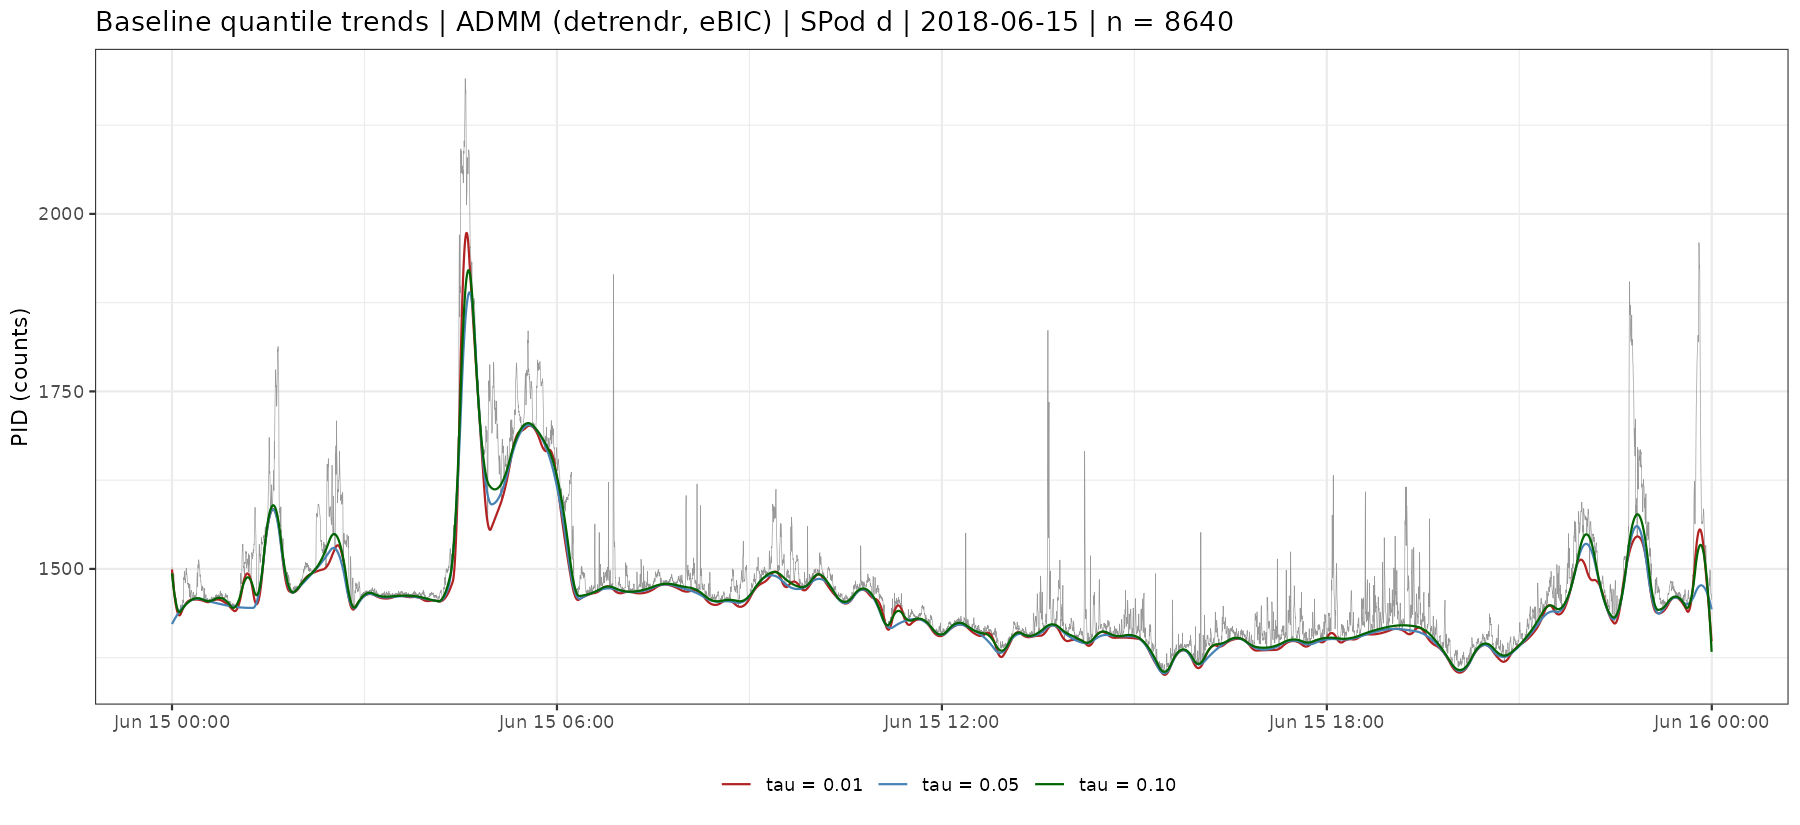
\includegraphics[width=\textwidth]{figures/spod_quantiles_admm}
		\caption{Baseline trends at $\tau \in \{0.01, 0.05, 0.1\}$, with $\lambda = 54.6$ at $\tau = 0.01$ and $\lambda = 1096.6$ at $\tau \in \{0.05, 0.1\}$ selected by eBIC.}
		\label{fig:spod_quantiles_admm}
	\end{subfigure}
	\par\medskip
	\begin{subfigure}{0.72\textwidth}
		\centering
		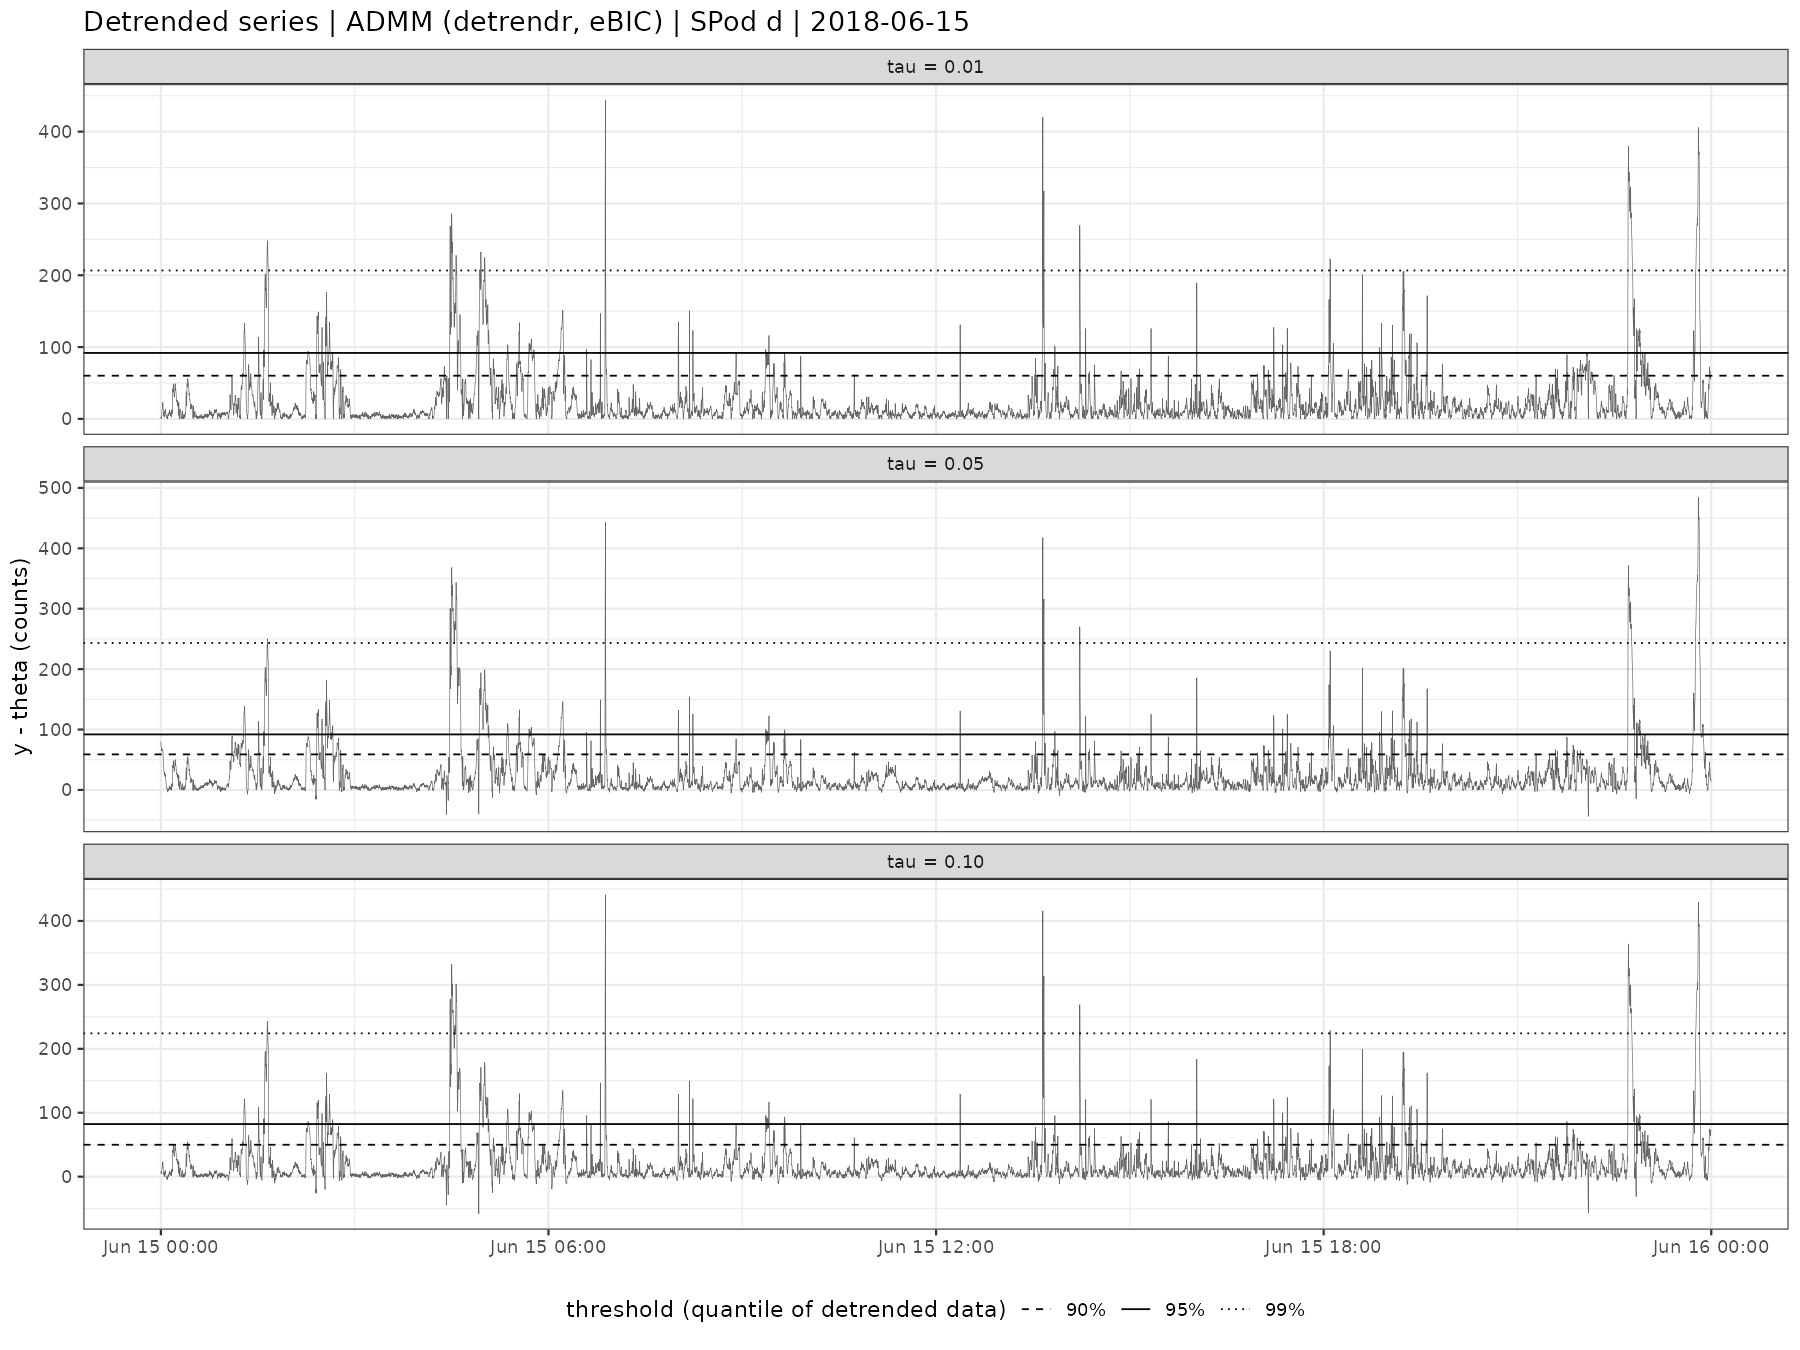
\includegraphics[width=\textwidth]{figures/spod_detrended_admm}
		\caption{Detrended series $\by - \widehat{\btheta}$ for the baselines in (a), one panel per quantile level. Horizontal lines mark the 90th (dashed), 95th (solid), and 99th (dotted) empirical percentiles of the detrended data.}
		\label{fig:spod_detrended_admm}
	\end{subfigure}
	\caption{Air quality data: ADMM benchmark fits \citep{brantley2020baseline} on the 10-second means ($n = 8{,}640$) of SPod \texttt{d}, June 15, 2018, with $\lambda$ selected by eBIC. The layout is that of Figures~\ref{fig:spod_quantiles_pmala} and~\ref{fig:spod_detrended_pmala}.}
	\label{fig:spod_admm}
\end{figure}

\clearpage

% ----------------------------------------------------------------------------
% Diagnostics from the earlier (k = 2, 60,000-iteration) Nile run.
% Parked here; the figure files are still in figures/.
% (Munich rent application removed from the paper 2026-10-28.)
% ----------------------------------------------------------------------------
\iffalse This appendix collects all plots for the real-data applications. The fits use the unchanged application P-MALA/Gibbs sampler for 60,000 iterations, with 10,000 burn-in iterations and thinning by 10.

\begin{figure}[p]
	\centering
	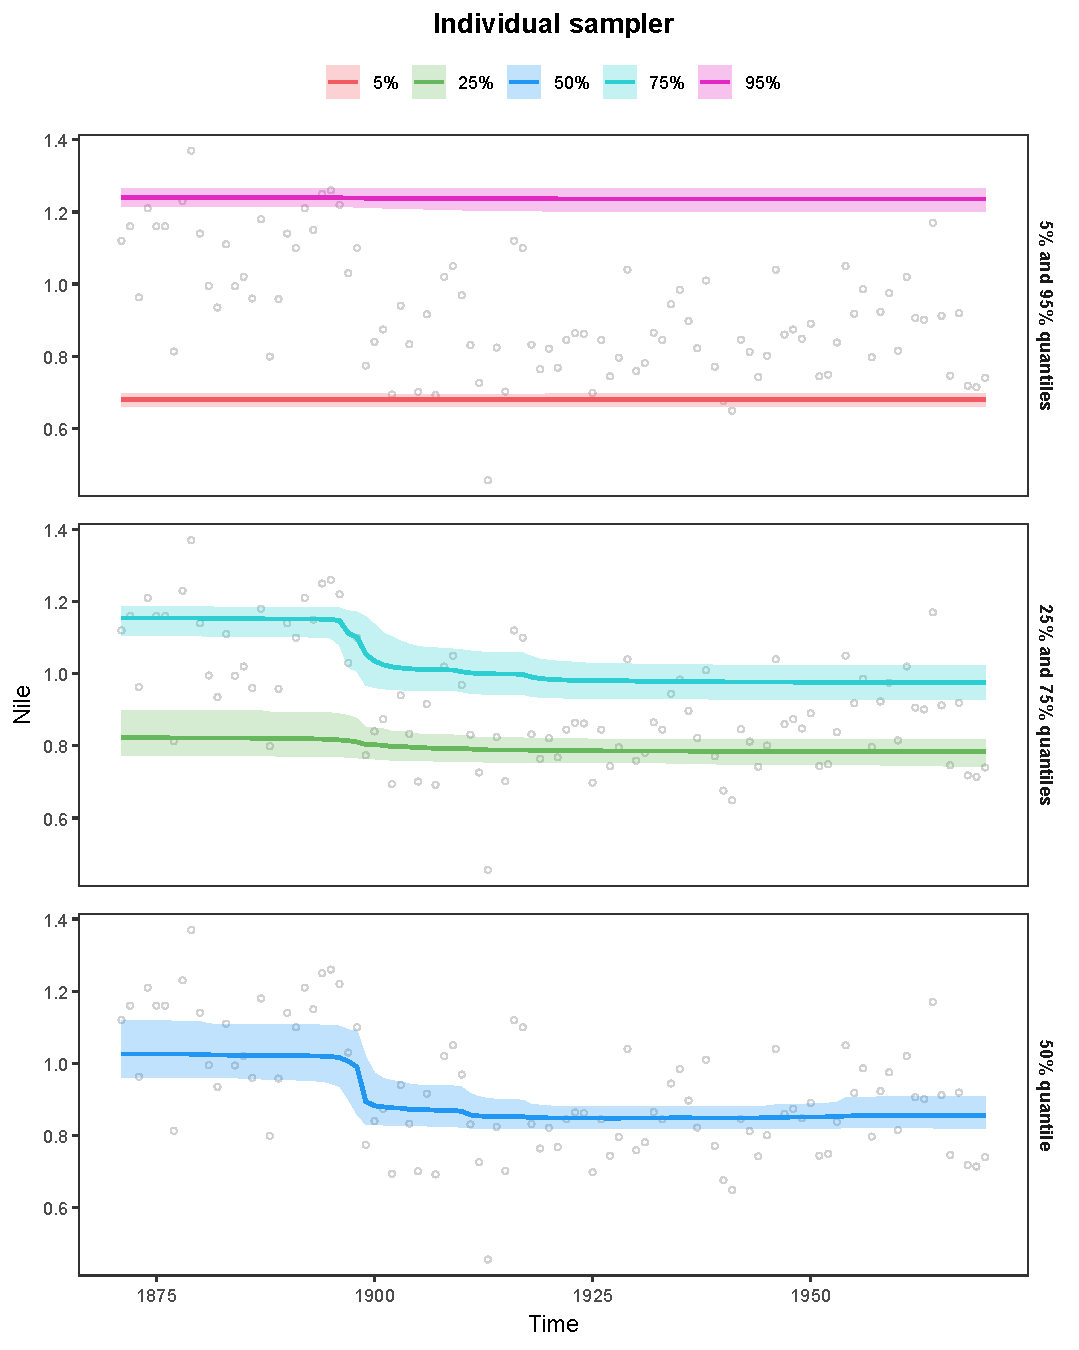
\includegraphics[width=0.75\textwidth,height=0.82\textheight,keepaspectratio]{figures/nile_individual_sampler}
	\caption{Individual P-MALA/Gibbs fits for the Nile data. Solid curves are posterior means and ribbons are 95\% pointwise credible intervals from the 5,000 retained draws. Grey circles are the rescaled observations.}
	\label{fig:nile}
\end{figure}

\begin{figure}[p]
	\centering
	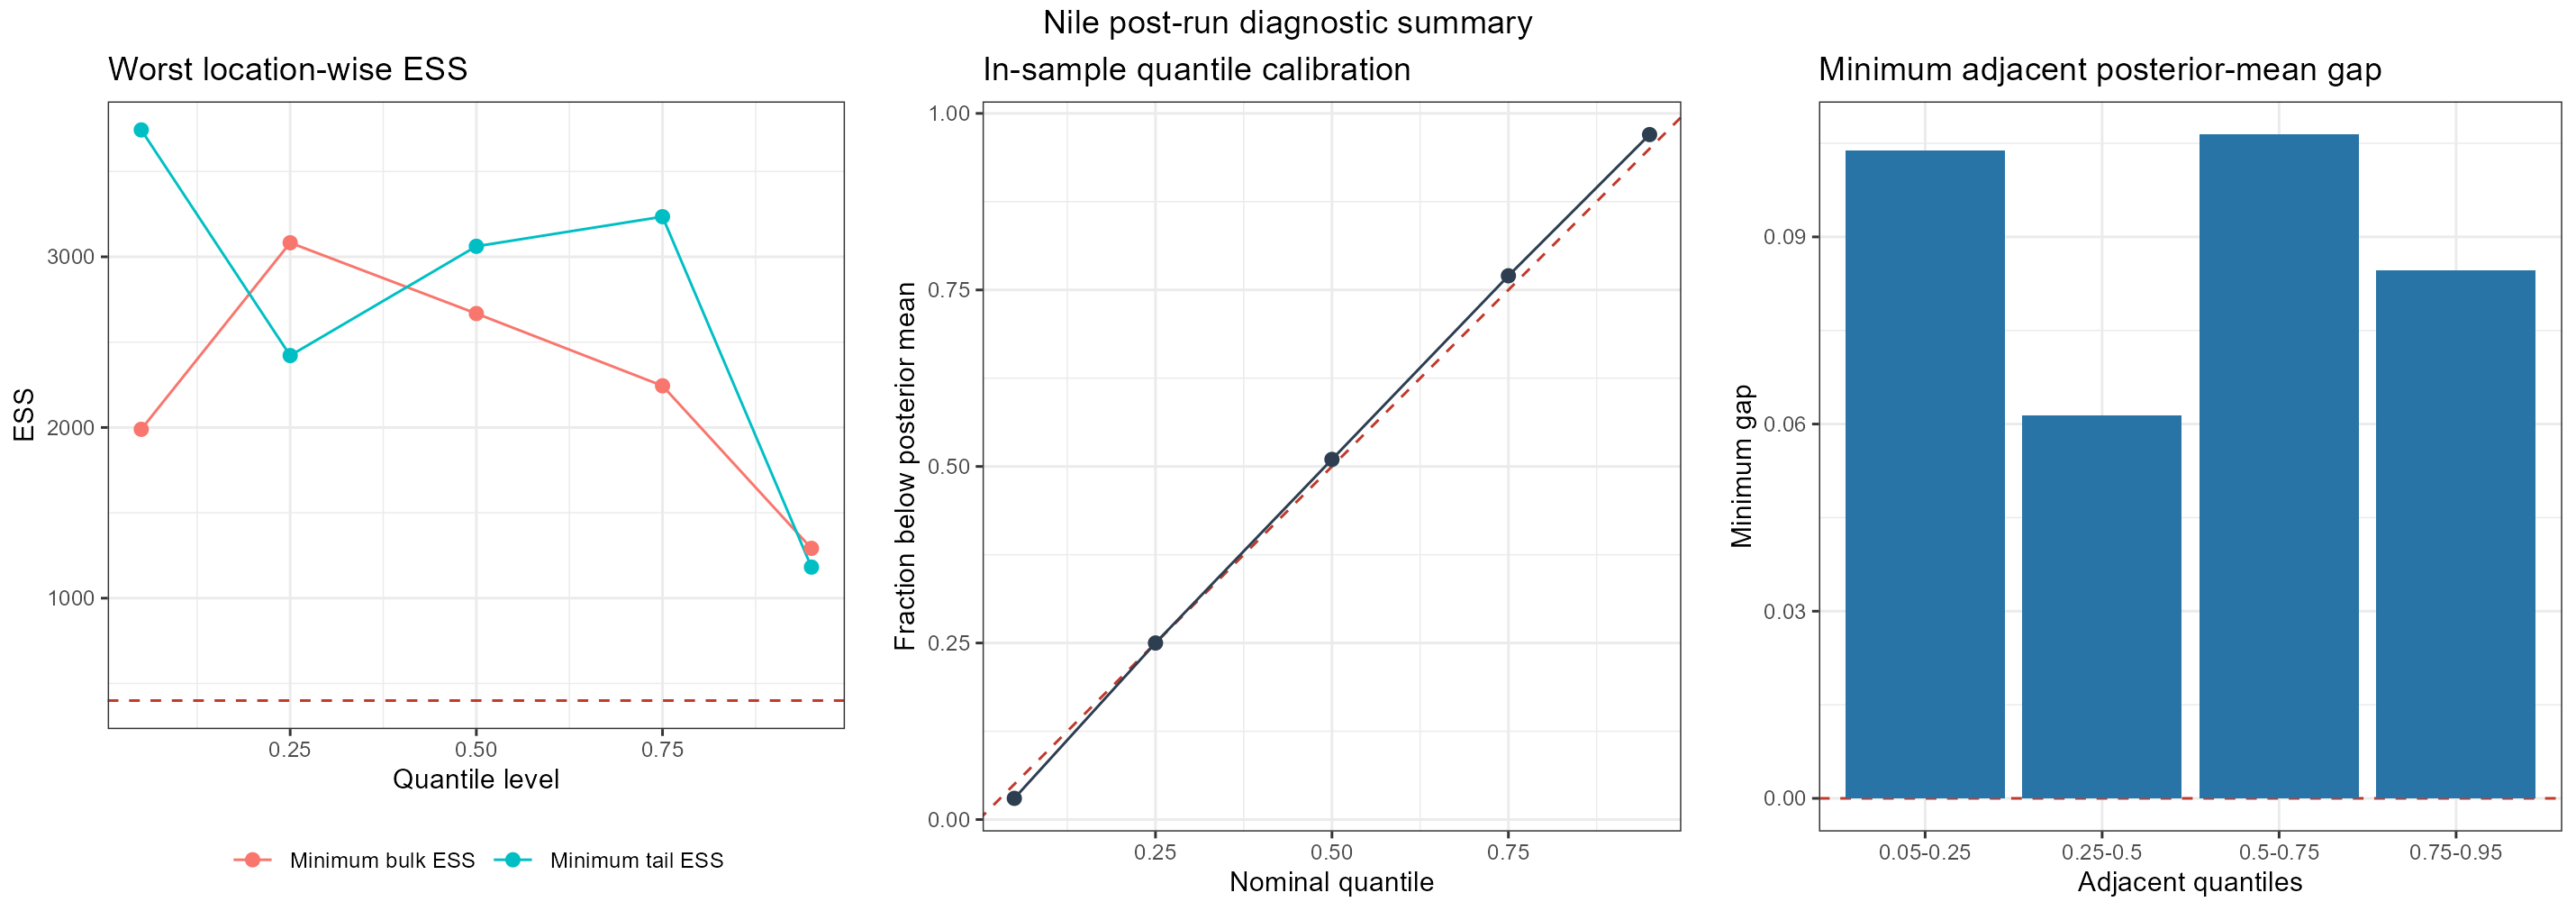
\includegraphics[width=0.75\textwidth]{figures/nile_diagnostic_summary}
	\caption{Nile post-run summaries: worst location-wise bulk and tail ESS, in-sample calibration, and minimum gap between adjacent posterior-mean curves. The ESS reference line is 400 and the calibration reference is the identity line.}
	\label{fig:app_diag_summary}
\end{figure}

\begin{figure}[p]
	\centering
	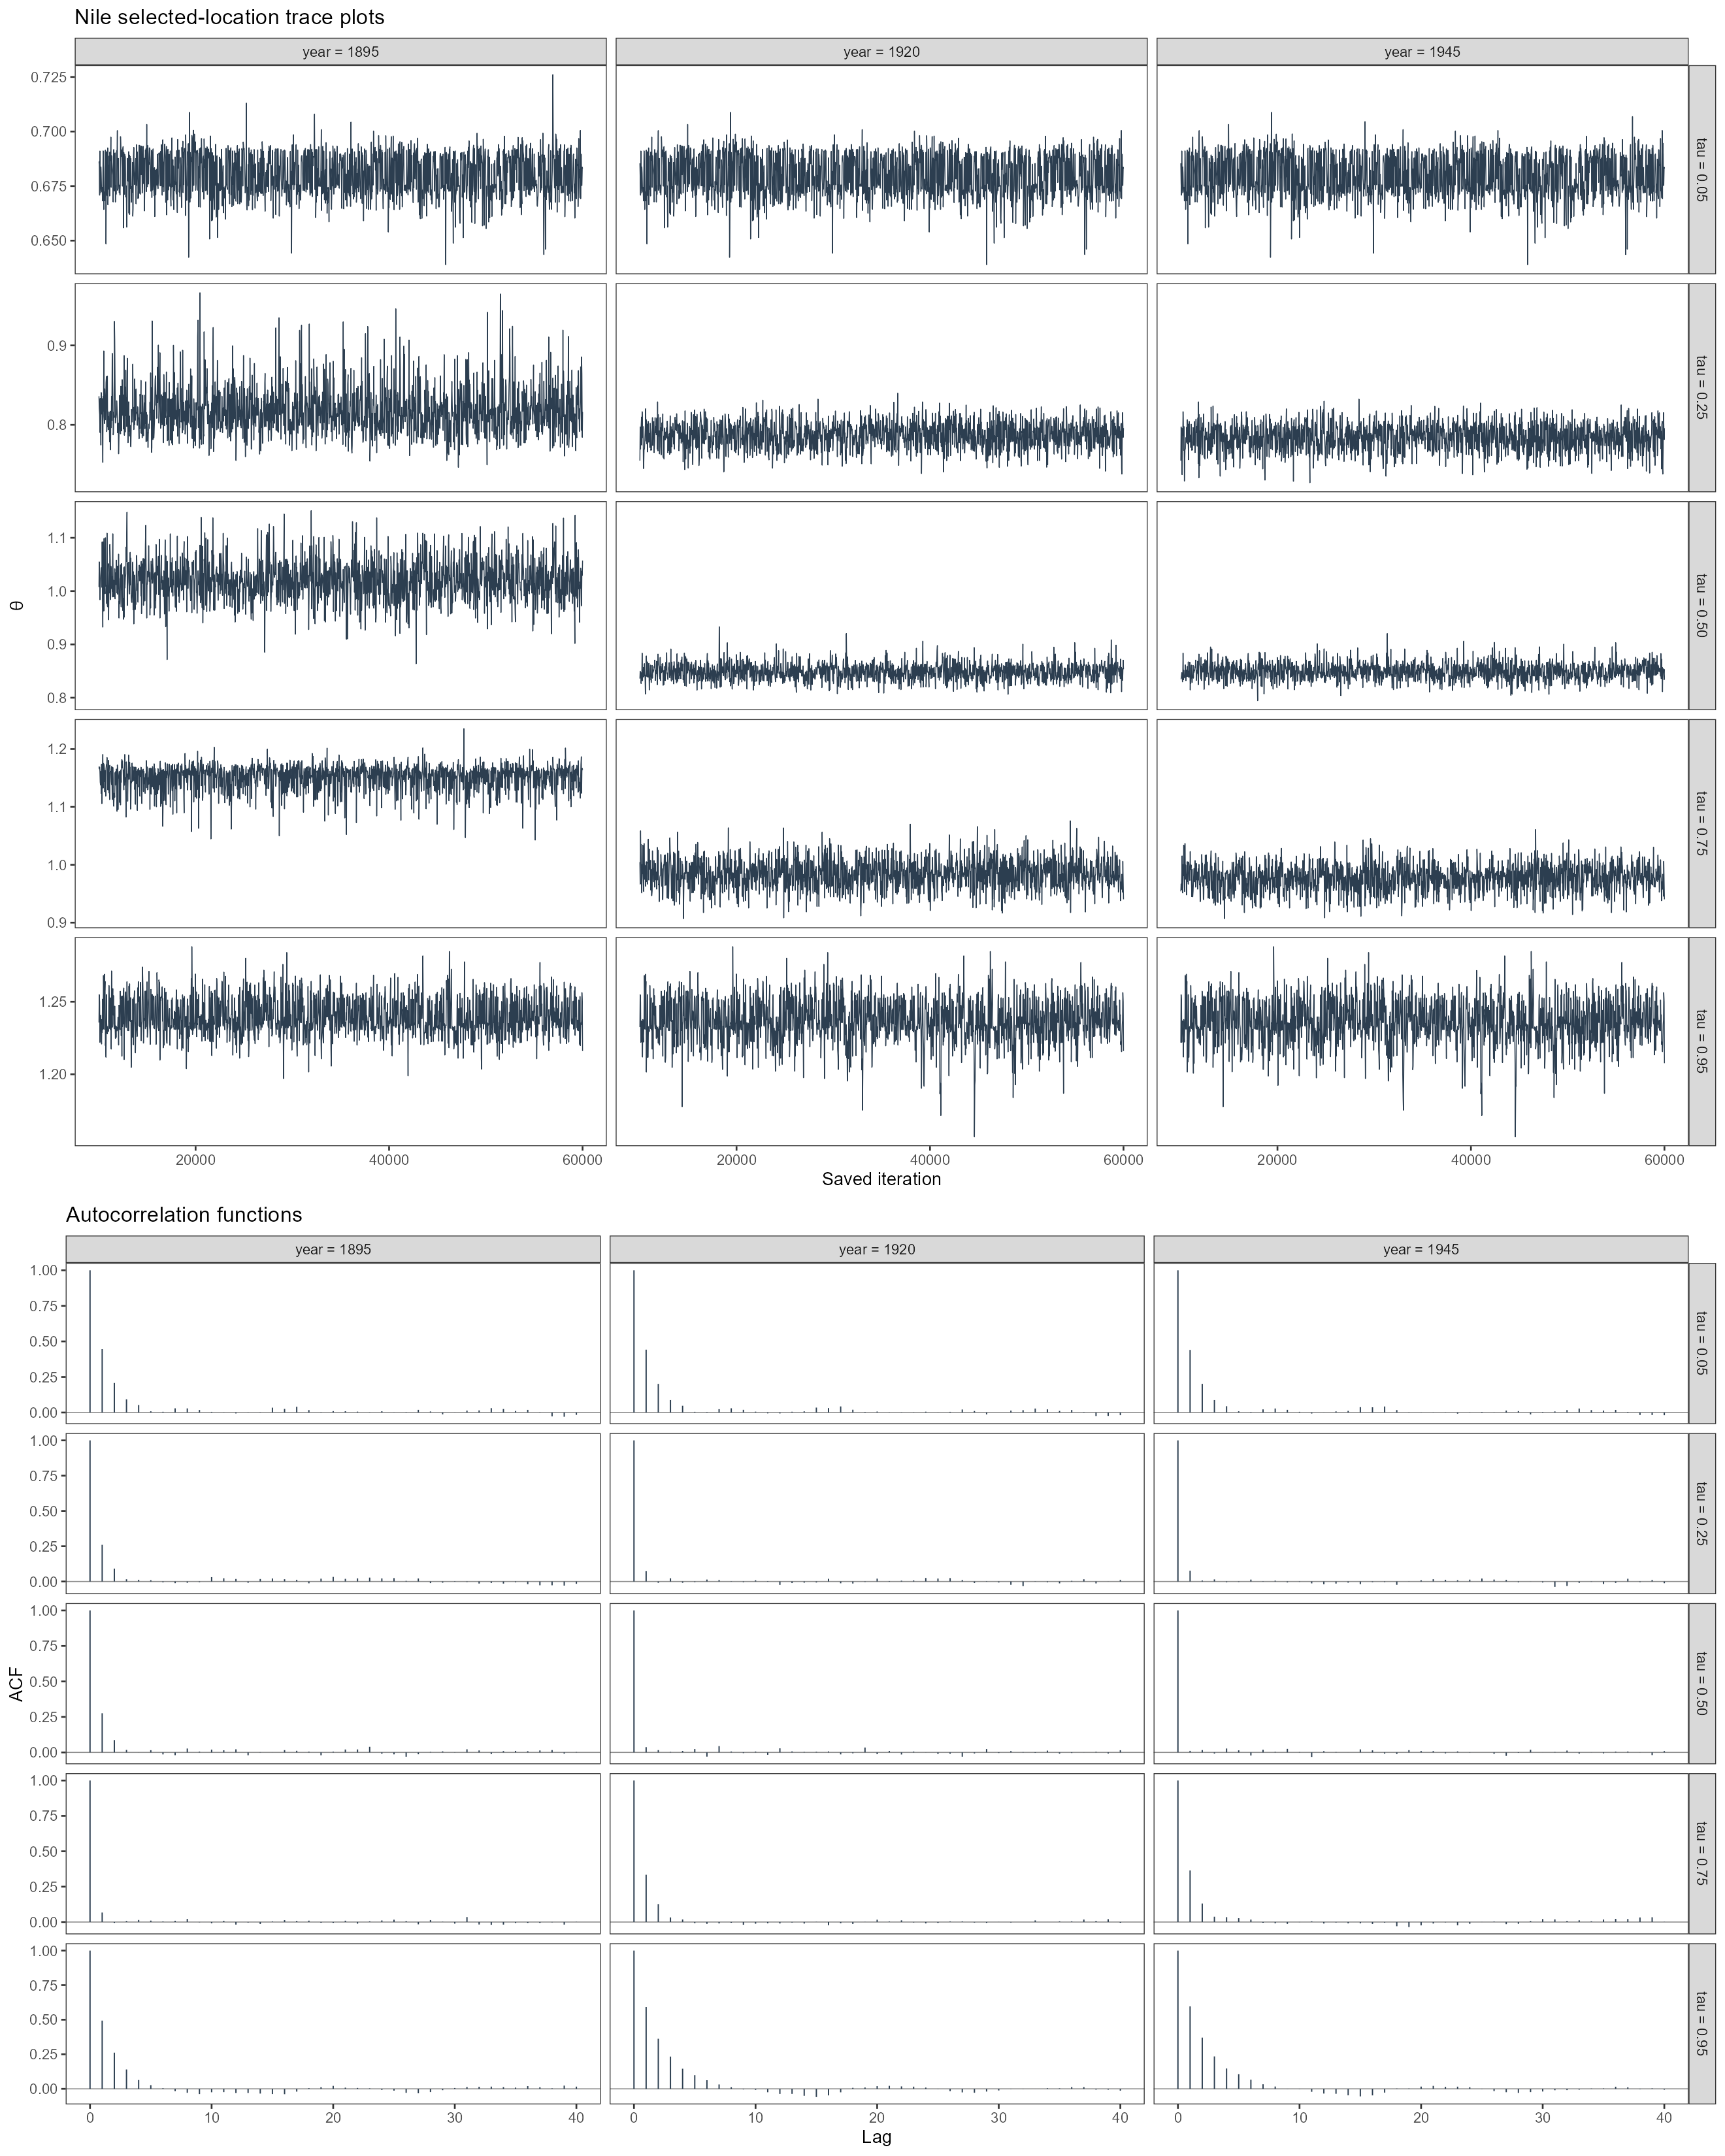
\includegraphics[width=0.75\textwidth,height=0.88\textheight,keepaspectratio]{figures/nile_trace_acf_diagnostics}
	\caption{Nile coefficient trace and autocorrelation diagnostics at representative years 1895, 1920, and 1945 for all five quantile levels. The horizontal scale of the trace panels is the original Gibbs iteration, so adjacent plotted values are ten iterations apart.}
	\label{fig:nile_trace_acf}
\end{figure}

\begin{figure}[p]
	\centering
	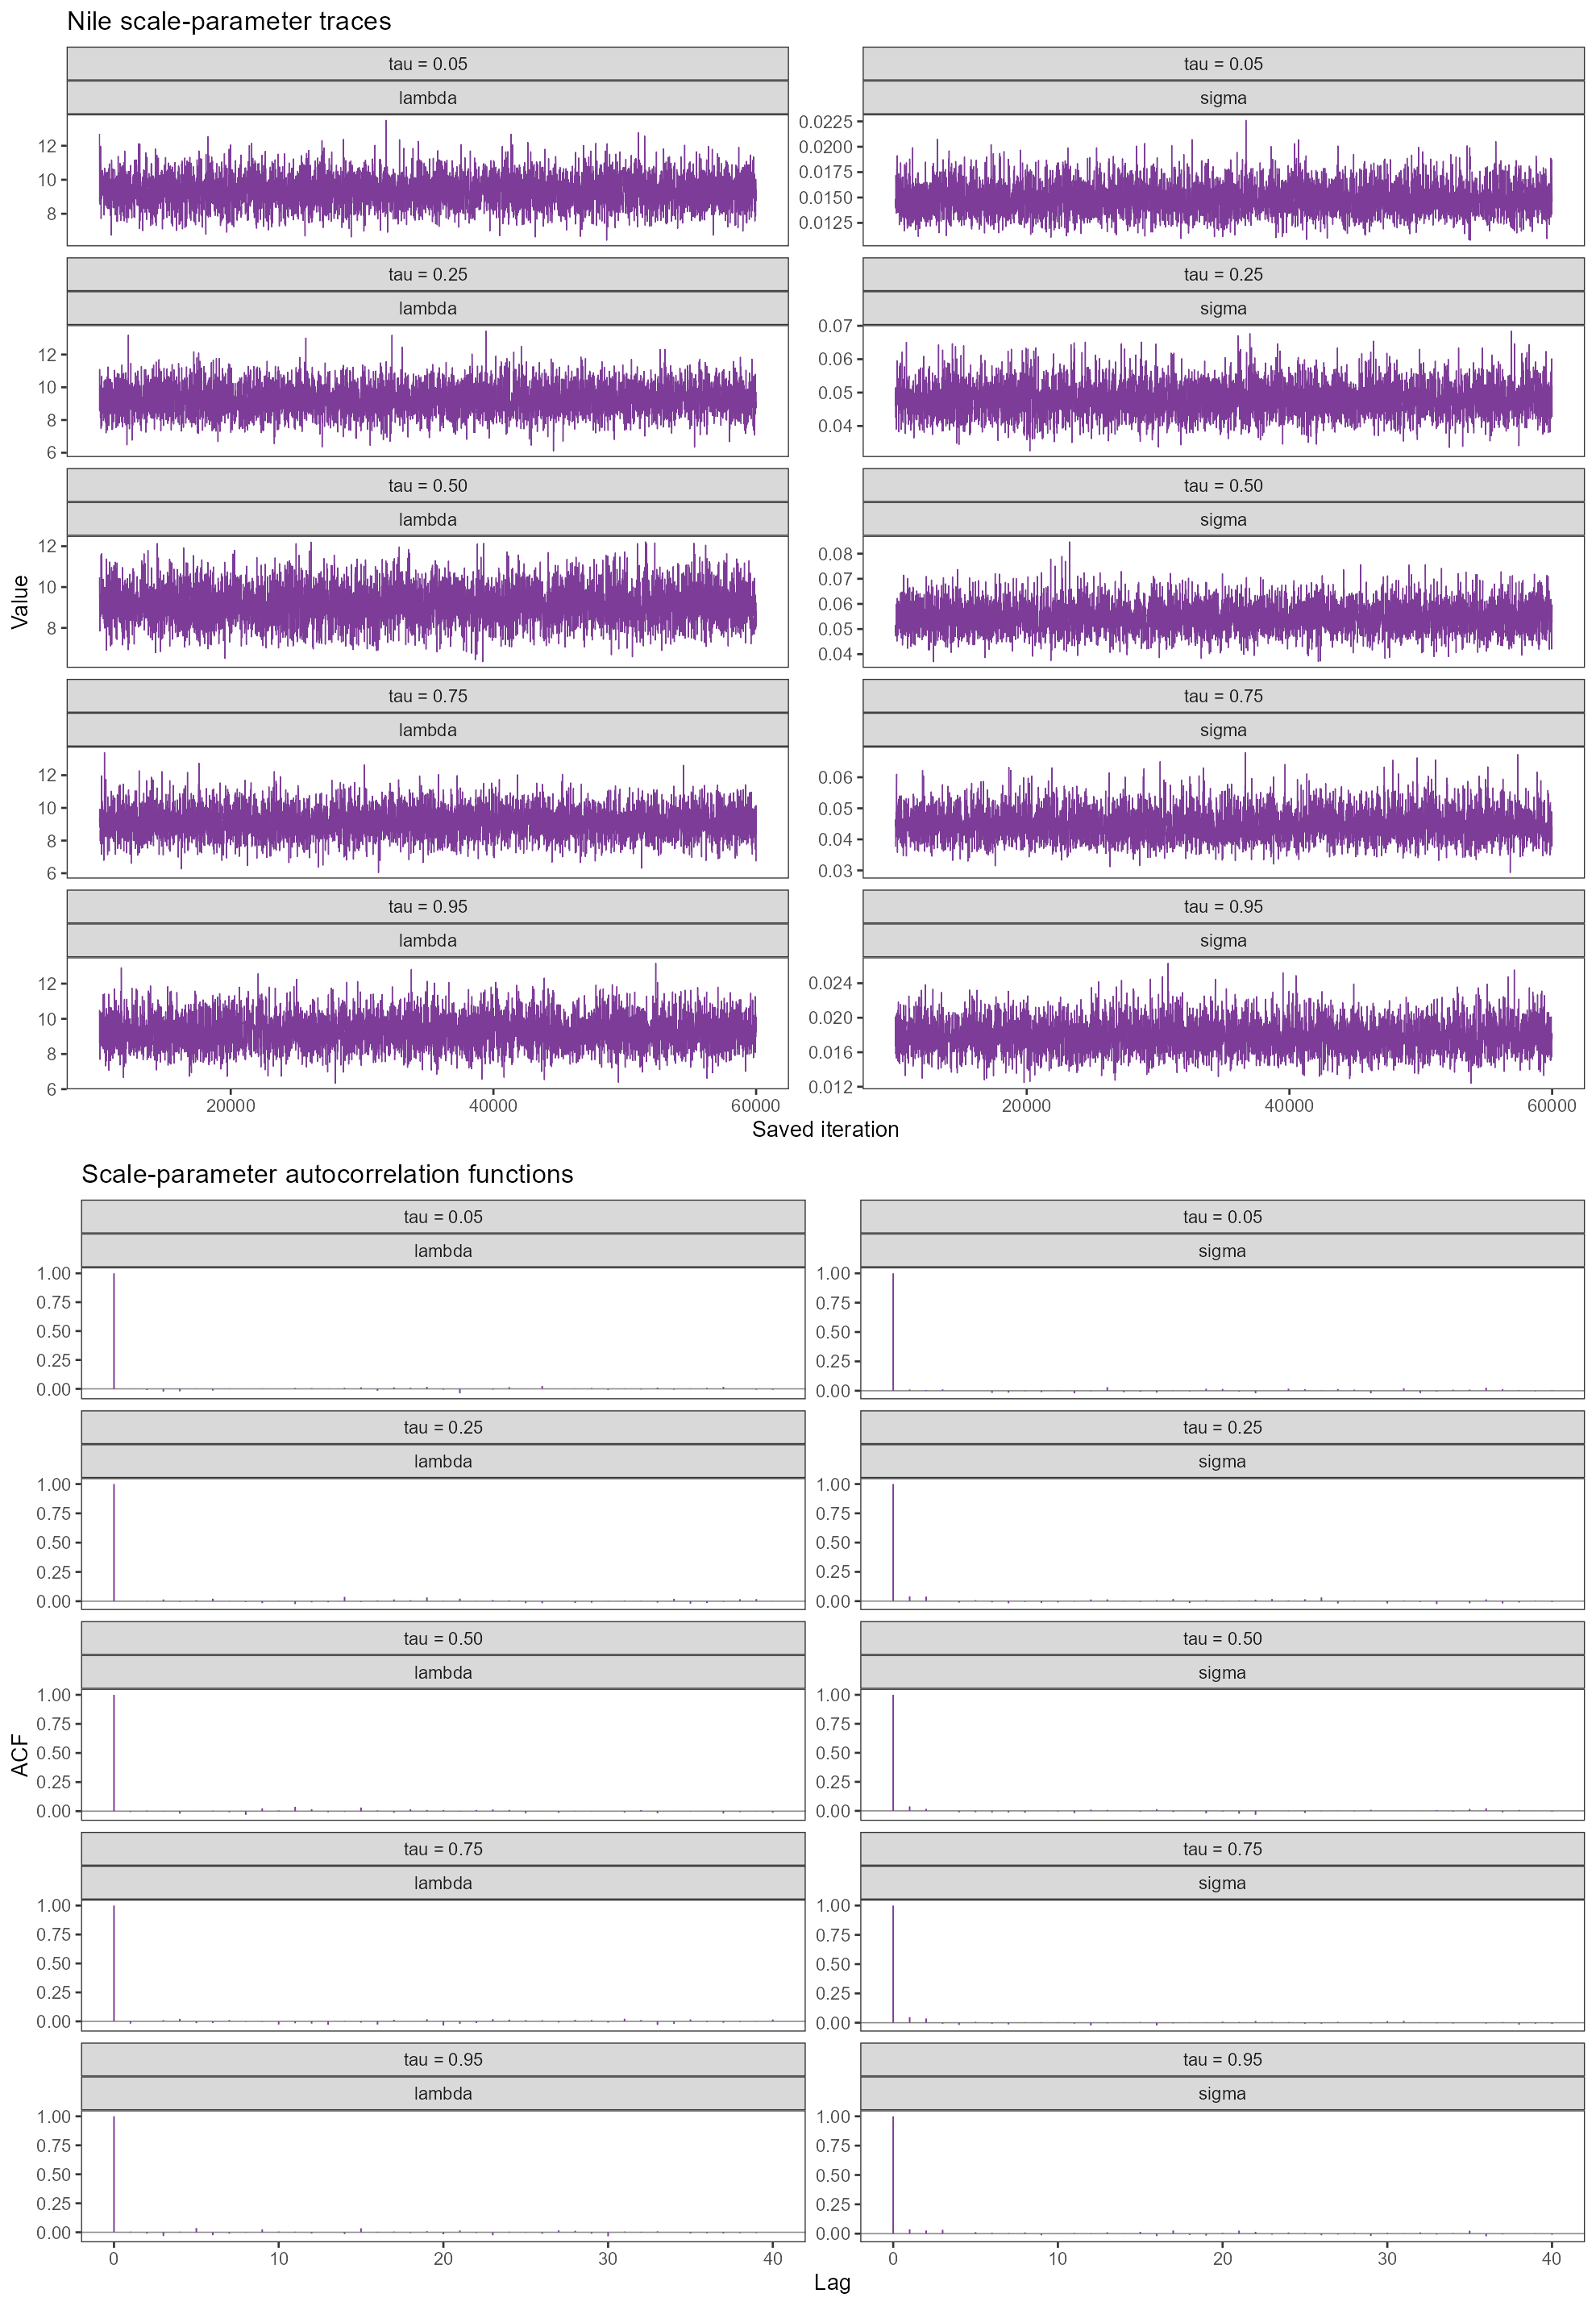
\includegraphics[width=0.75\textwidth,height=0.88\textheight,keepaspectratio]{figures/nile_scale_trace_acf_diagnostics}
	\caption{Nile trace and autocorrelation diagnostics for \(\lambda\) and \(\sigma\). Both scale-parameter chains mix rapidly and show no visible drift.}
	\label{fig:nile_scale_trace_acf}
\end{figure}

\begin{figure}[p]
	\centering
	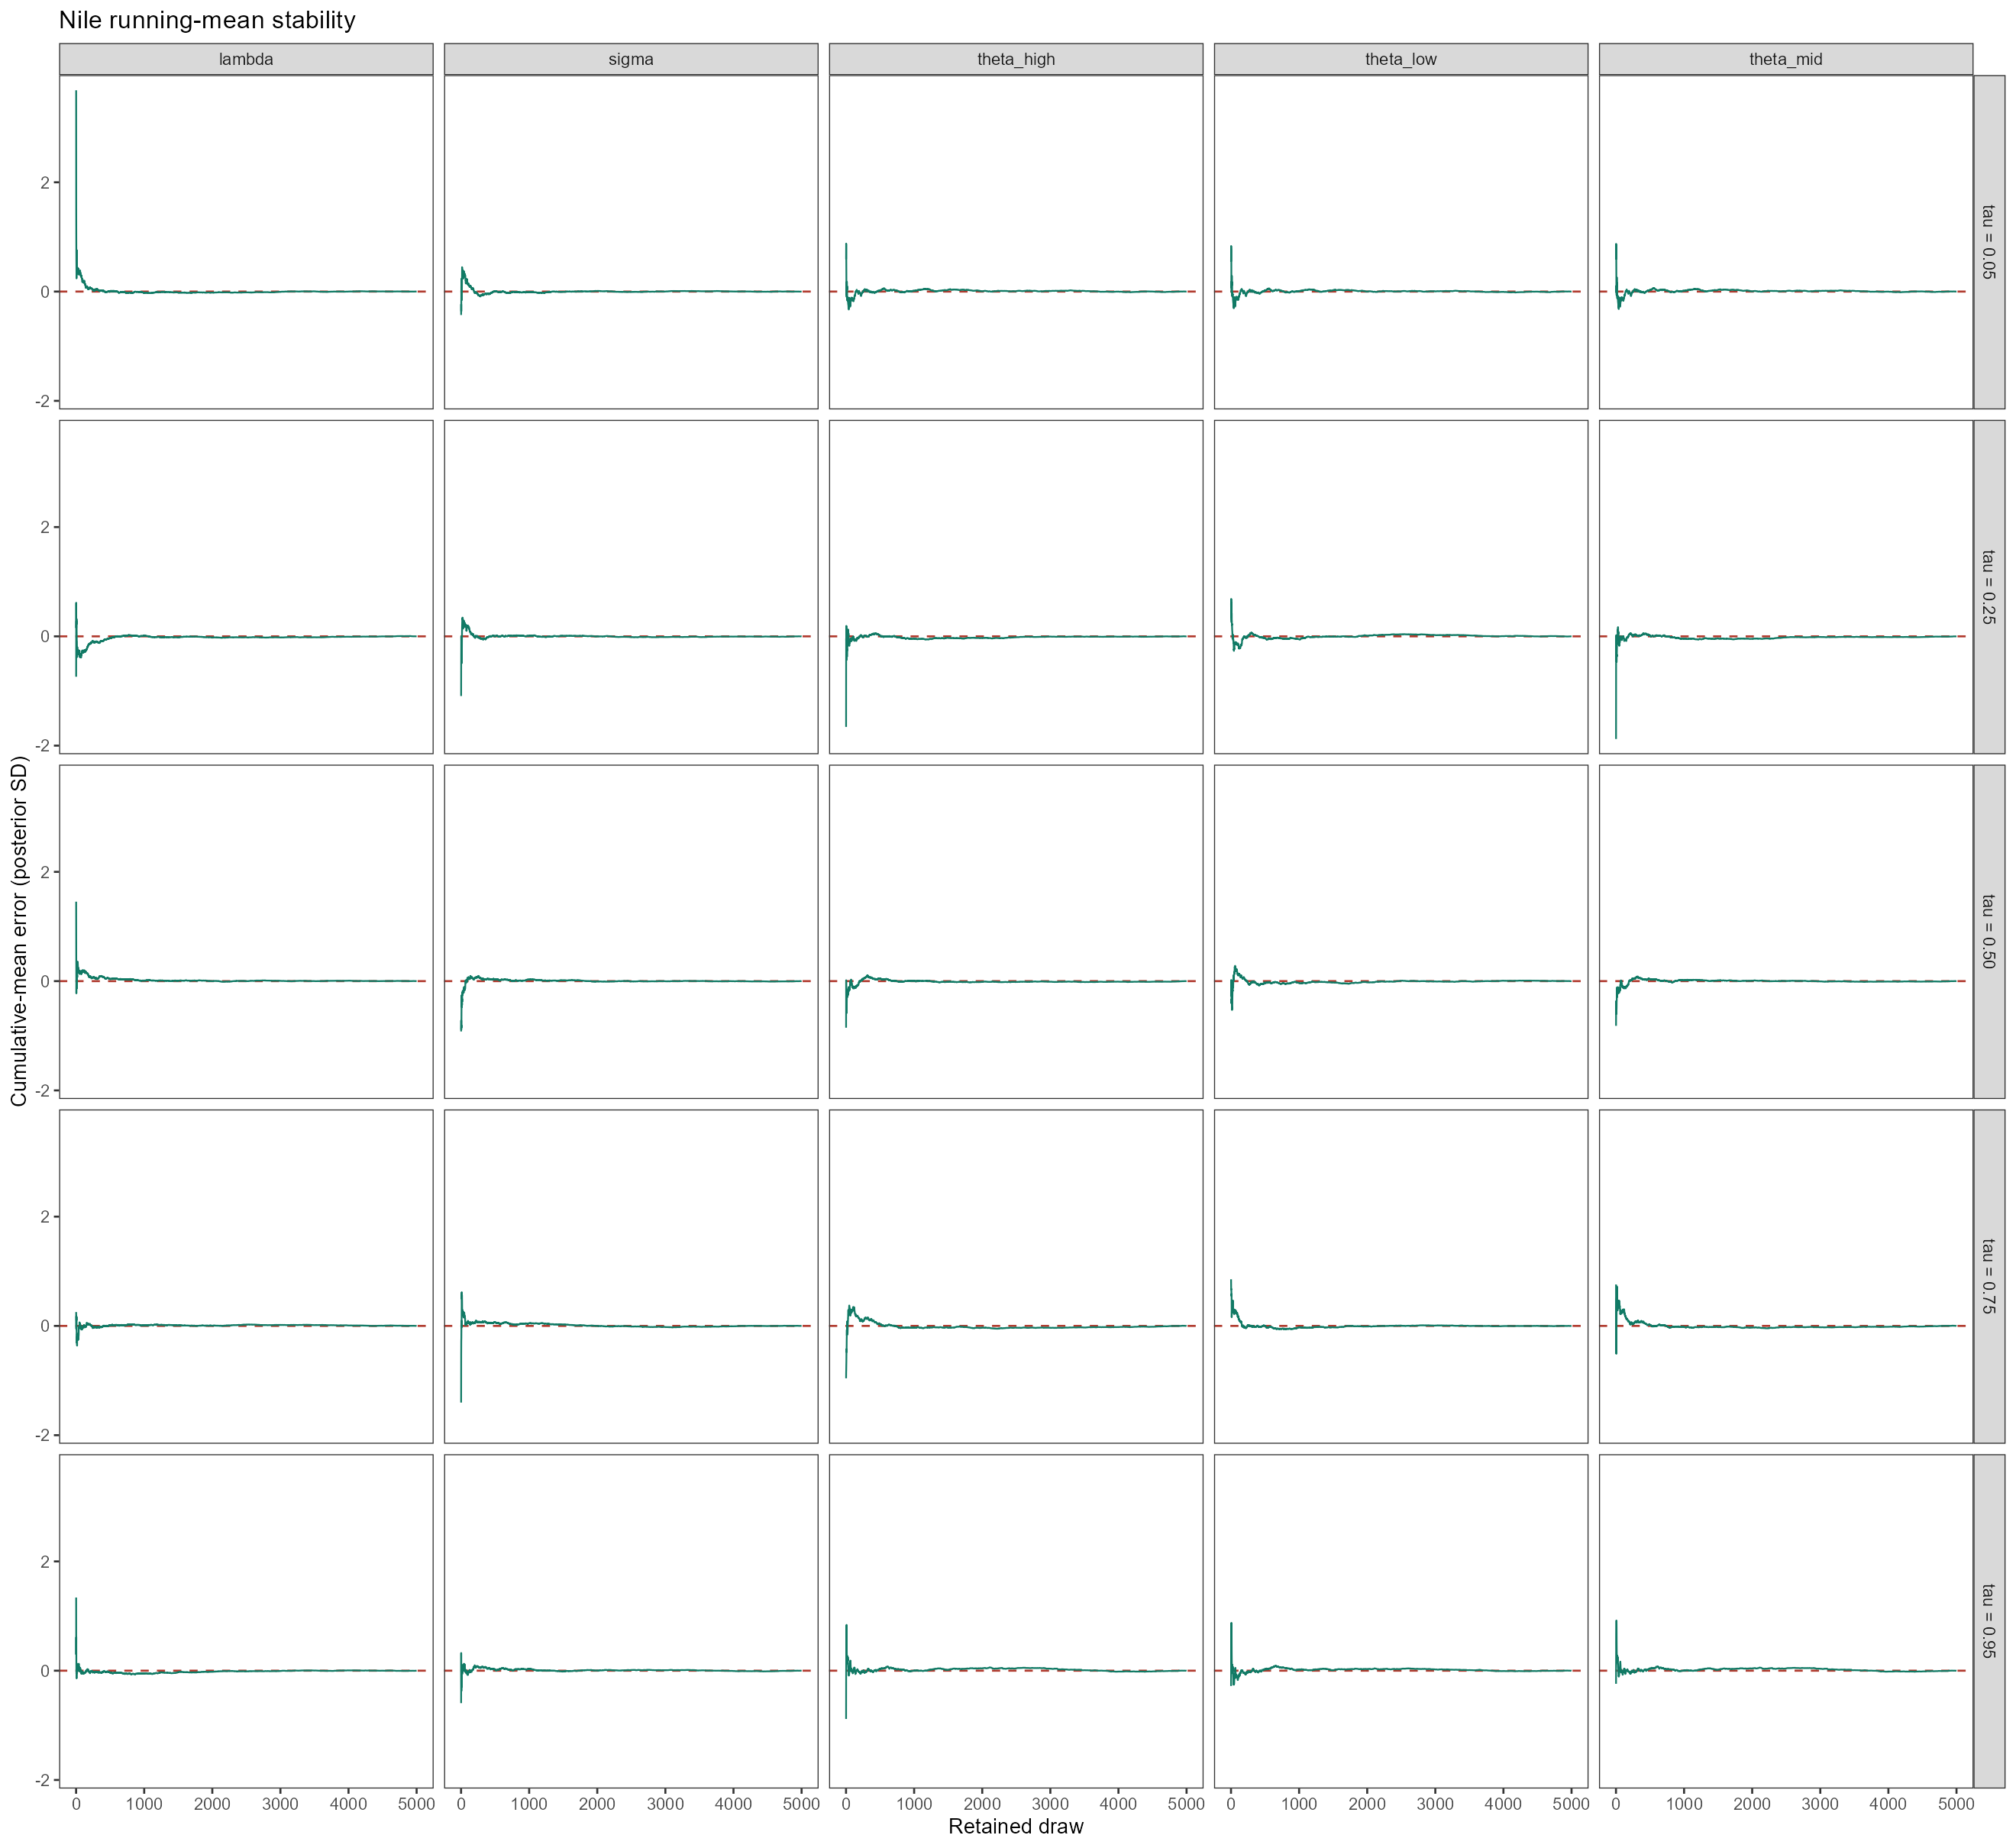
\includegraphics[width=0.75\textwidth,height=0.88\textheight,keepaspectratio]{figures/nile_running_mean_stability}
	\caption{Nile standardized cumulative-mean diagnostics. Each curve is the cumulative mean minus its final posterior mean, divided by the posterior standard deviation; the dashed line is zero.}
	\label{fig:nile_running_mean}
\end{figure}

\fi

\subsection{Growth Centiles}
\label{app:growth}

This appendix reports the growth-chart fits of Section~\ref{sec:app:growth} that are not shown there: the individual sampler for girls and the LMS centiles \citep{cole1992smoothing} for boys and girls. The P-MALA settings are those of Section~\ref{sec:app:growth}: $k = 2$, $\lambda \sim \mathrm{Gamma}(1,\sqrt{G})$, 6{,}000 iterations with 1{,}000 burn-in, and one independent run per level. The LMS curves are the 10th, 30th, 50th, 70th, and 90th centiles of the fitted Box--Cox Cole--Green distribution, evaluated on the same 0.1-year age grid.

\begin{figure}[htbp]
	\centering
	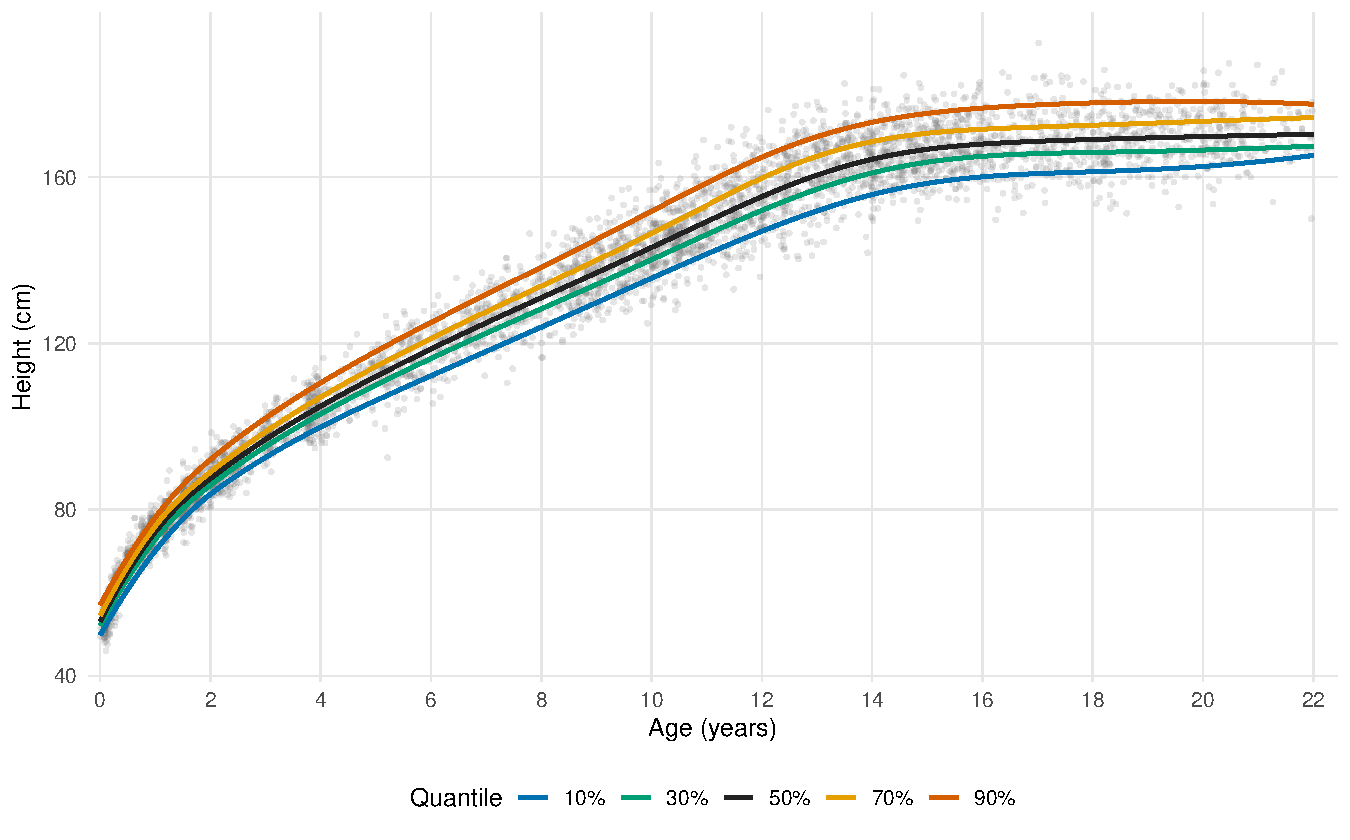
\includegraphics[width=0.75\textwidth]{figures/growth_pmala_girls}
	\caption{Individual P-MALA/Gibbs fits for the height of 5{,}190 Dutch girls (Fifth Dutch Growth Study, 2009) at $\tau \in \{0.1, 0.3, 0.5, 0.7, 0.9\}$, $k = 2$. Curves are posterior means on the 0.1-year age grid; grey circles are the individual measurements. Each level is fitted independently.}
	\label{fig:growth_girls}
\end{figure}

\begin{figure}[htbp]
	\centering
	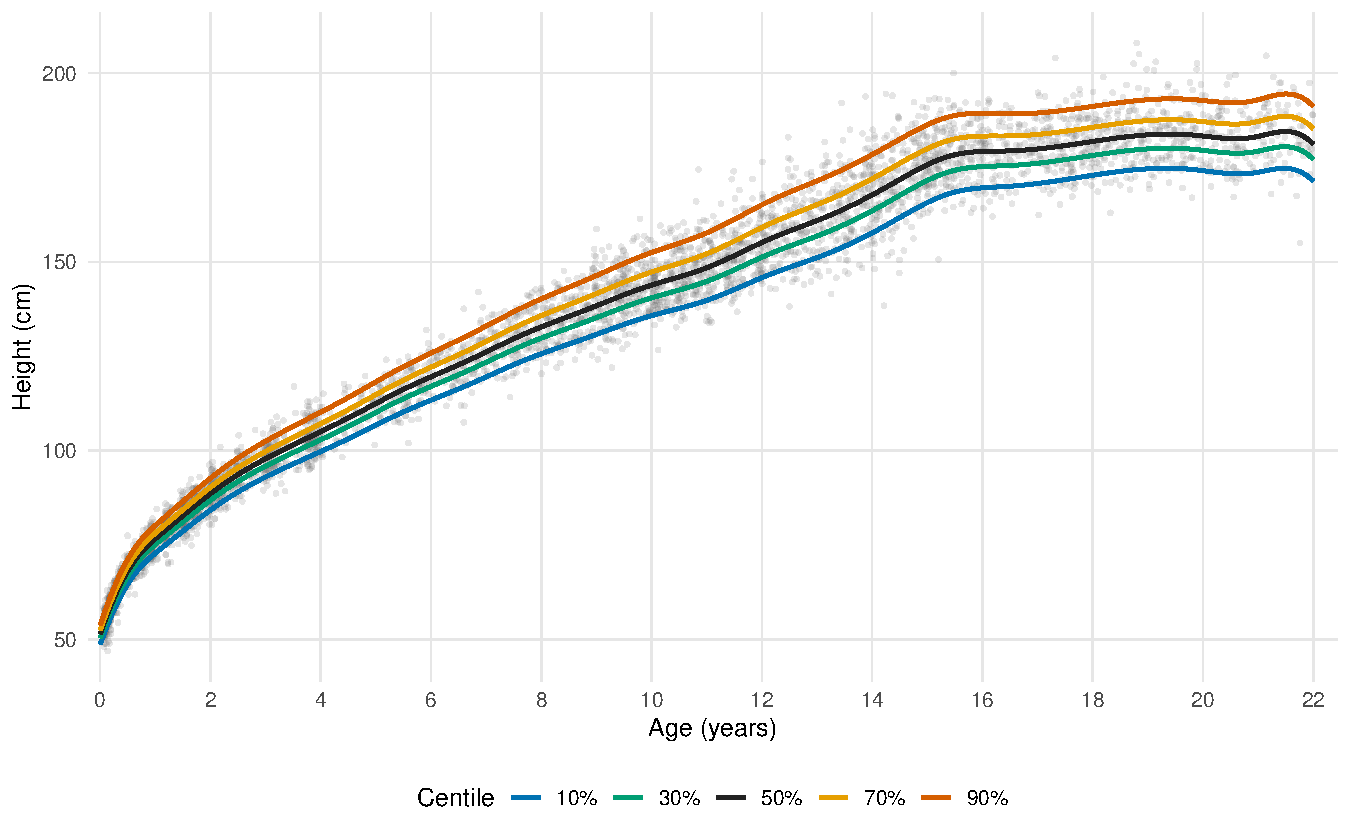
\includegraphics[width=0.75\textwidth]{figures/growth_lms_boys}
	\caption{LMS centiles for the height of 4{,}817 Dutch boys (Fifth Dutch Growth Study, 2009): the 10th, 30th, 50th, 70th, and 90th centiles of the fitted Box--Cox Cole--Green distribution, whose median, coefficient of variation, and Box--Cox power are smooth in age.}
	\label{fig:growth_lms_boys}
\end{figure}

\begin{figure}[htbp]
	\centering
	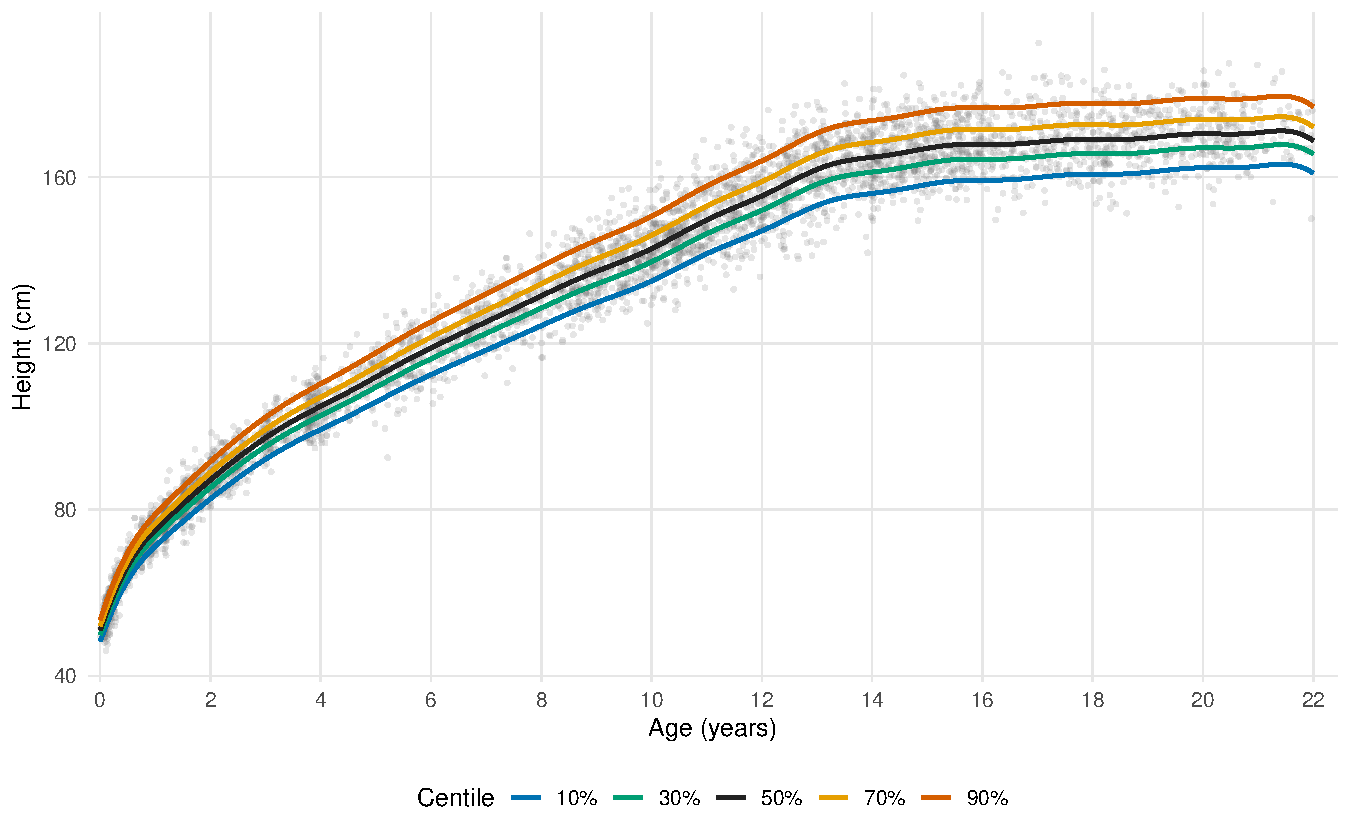
\includegraphics[width=0.75\textwidth]{figures/growth_lms_girls}
	\caption{LMS centiles for the height of 5{,}190 Dutch girls (Fifth Dutch Growth Study, 2009), with the layout of Figure~\ref{fig:growth_lms_boys}.}
	\label{fig:growth_lms_girls}
\end{figure}

\clearpage
%\nocite{*}
\bibliographystyle{apalike}
\bibliography{references}
\end{document}
